\chapter[The lead-up to the Sturtian Snowball Earth: Neoproterozoic chemostratigraphy time-calibrated by the Tambien Group of Ethiopia][Tambien Group]{The lead-up to the Sturtian Snowball Earth: Neoproterozoic chemostratigraphy time-calibrated by the Tambien Group of Ethiopia}

\section{Abstract}

The Tonian-Cryogenian Tambien Group of northern Ethiopia is a mixed carbonate-siliciclastic sequence that culminates in glacial deposits associated with the first of the Cryogenian glaciations - the Sturtian `Snowball Earth.' Tambien Group deposition occurred atop arc volcanics and volcaniclastics of the Tsaliet Group. New U-Pb isotope dilution thermal ionization mass spectrometry (ID-TIMS) dates demonstrate that the transition between the Tsaliet and Tambien groups occurred at ca. 820~Ma in western exposures and ca. 795~Ma in eastern exposures, which is consistent with west to east arc migration and deposition in an evolving back-arc basin. The presence of intercalated tuffs suitable for high-precision geochronology within the Tambien Group enable temporal constraints on stratigraphic datasets of the interval preceding, and leading into, the Sturtian Glaciation. Recently discovered exposures of Sturtian glacial deposits and underlying Tambien Group strata in the Samre Fold-Thrust Belt present the opportunity to further utilize this unique association of tuffs and carbonate lithofacies. U-Pb ID-TIMS ages from zircons indicate that Tambien Group carbonates were deposited from ca. 820~Ma until 0 to 2~Myr before the onset of the Sturtian Glaciation, making the group host to a relatively complete carbonate stratigraphy leading into this glaciation. New \dC and \SrSr data and U-Pb ID-TIMS ages from the Tambien Group are used in conjunction with previously published isotopic and geochronologic data to construct newly time-calibrated composite Tonian carbon and strontium isotope curves. Tambien Group \dC data and U-Pb ID-TIMS ages reveal that a pre-Sturtian sharp negative \dC excursion (referred to as the Islay anomaly in the literature) precedes the Sturtian Glaciation by $\sim$18~Myr, is synchronous in at least two separate basins, and is followed by a prolonged interval of positive \dC values. The composite Tonian \SrSr curve shows that, following an extended interval of low and relatively invariant values, inferred seawater \SrSr rose ca. 880-770~Ma, and then decreased to the ca. 717~Ma initiation of the Sturtian Glaciation. These data, when combined with a simple global weathering model and analyses of the timing and paleolatitude of large igneous province eruptions and arc accretion events, suggest that the \SrSr increase was influenced by increased subaerial weathering of radiogenic lithologies as Rodinia rifted apart at low latitudes. The following \SrSr decrease is consistent with enhanced subaerial weathering of arc lithologies accreting in the tropics over tens of millions of years, lowering \pCOtwo and contributing to the initiation of the Sturtian Glaciation.

\section{Introduction}

Life and climate evolved dramatically during the Tonian Period (1000-717~Ma). Sedimentary rocks from this period record the diversification of eukaryotic life (e.g. \citealp{Knoll2006a, Butterfield2015a}), large-scale fluctuations of the carbon cycle as recorded by the \dC of shallow marine carbonates (e.g. \citealp{Halverson2005a}), and major changes to paleogeography (e.g. \citealp{Li2008a, Li2013a, Merdith2017a}) during the lead-up to severe Cryogenian glaciations. Understanding global change leading up to these glaciations is critical for interpreting the boundary conditions that allowed these extreme environmental conditions to occur, especially since no ice sheets are known to have existed for $\sim$1.5~Gyr between ca. 2.2~Ga Paleoproterozoic glaciation \citep{Evans1997a} and the ca. 717~Ma start of the Cryogenian glaciations \citep{Macdonald2010a, MacLennan2018a}.

The Tonian-Cryogenian Tambien Group of the Tigray region of northern Ethiopia is a mixed carbonate-siliciclastic sequence deposited in an arc-proximal basin that culminates in glacial deposits associated with the first of the Cryogenian glaciations - the Sturtian `Snowball Earth' \citep{Beyth2003a, Miller2003a, Swanson-Hysell2015a, MacLennan2018a}. The presence of intercalated tuffs suitable for high-precision U-Pb isotope dilution thermal ionization mass spectrometry (ID-TIMS) geochronology leading into the glaciation makes the Tambien Group a target for temporally constraining stratigraphic and isotopic datasets of the interval preceding, and leading into, the Sturtian Glaciation. For example, large-scale carbon isotopic change ca. 810-790~Ma (the Bitter Springs stage) was inferred to be globally synchronous on the basis of U-Pb ID-TIMS dates from western exposures of lower Tambien Group rocks in Ethiopia \citep{Swanson-Hysell2015a} in conjunction with U-Pb ID-TIMS dates from Fifteenmile Group rocks in Canada \citep{Macdonald2010a}. \citet{Swanson-Hysell2015a} also developed a lithostratigraphic framework for the Tambien Group that built on the prior work of \citet{Beyth1972a}, \citet{Hailu1975a}, and \citet{Garland1980a}, and proposed that upper Tambien Group formations only had been documented in the core of the Negash Syncline at that time. However, a lack of geochronology from these strata limited the potential to test this proposed framework and develop time-calibrated stratigraphic records.

Subsequent fieldwork led to the discovery of abundant previously unstudied exposures of upper Tambien Group stratigraphy, including Sturtian glacial deposits, in the Samre Fold-Thrust Belt (Figs. \ref{fig:overview-map} and \ref{fig:Negash-Samre-maps}). These exposures provide the opportunity to produce lithostratigraphic, geochronologic, and chemostratigraphic data from the interval immediately preceding the Sturtian Glaciation. Geochronologic and \dC data from these Samre Fold-Thrust Belt exposures provide evidence for the global synchronicity of both a large-scale carbon isotopic excursion ca. 735~Ma (often referred to as the Islay anomaly in the literature, although \citealp{Fairchild2018a} proposed that the term should be deprecated), and separately the initiation of the Sturtian Glaciation \citep{MacLennan2018a}. Tambien Group carbonates were deposited from ca. 820~Ma until 0 to 2~Myr before the onset of the Sturtian Glaciation, making the group host to what may be the most demonstrably complete carbonate stratigraphy leading into this glaciation reported to date from anywhere in the world \citep{MacLennan2018a}.

This study presents new lithostratigraphic and chemostratigraphic (\dC, \dO, and \SrSr) data, and additional U-Pb ID-TIMS dates from zircons, from the lower Tambien Group in the Mai Kenetal Syncline and the upper Tambien Group in the Negash Syncline and the newly mapped Samre Fold-Thrust Belt. With these data, we construct the most complete and temporally well-constrained pre-Sturtian chemostratigraphic composite record to date, which we use to assess the nature of pre-glacial carbon isotope anomalies and the role of changing global weathering fluxes on the initiation of the Sturtian Glaciation.

\section{Geological Setting}

\begin{figure}[h!]
\begin{center}
	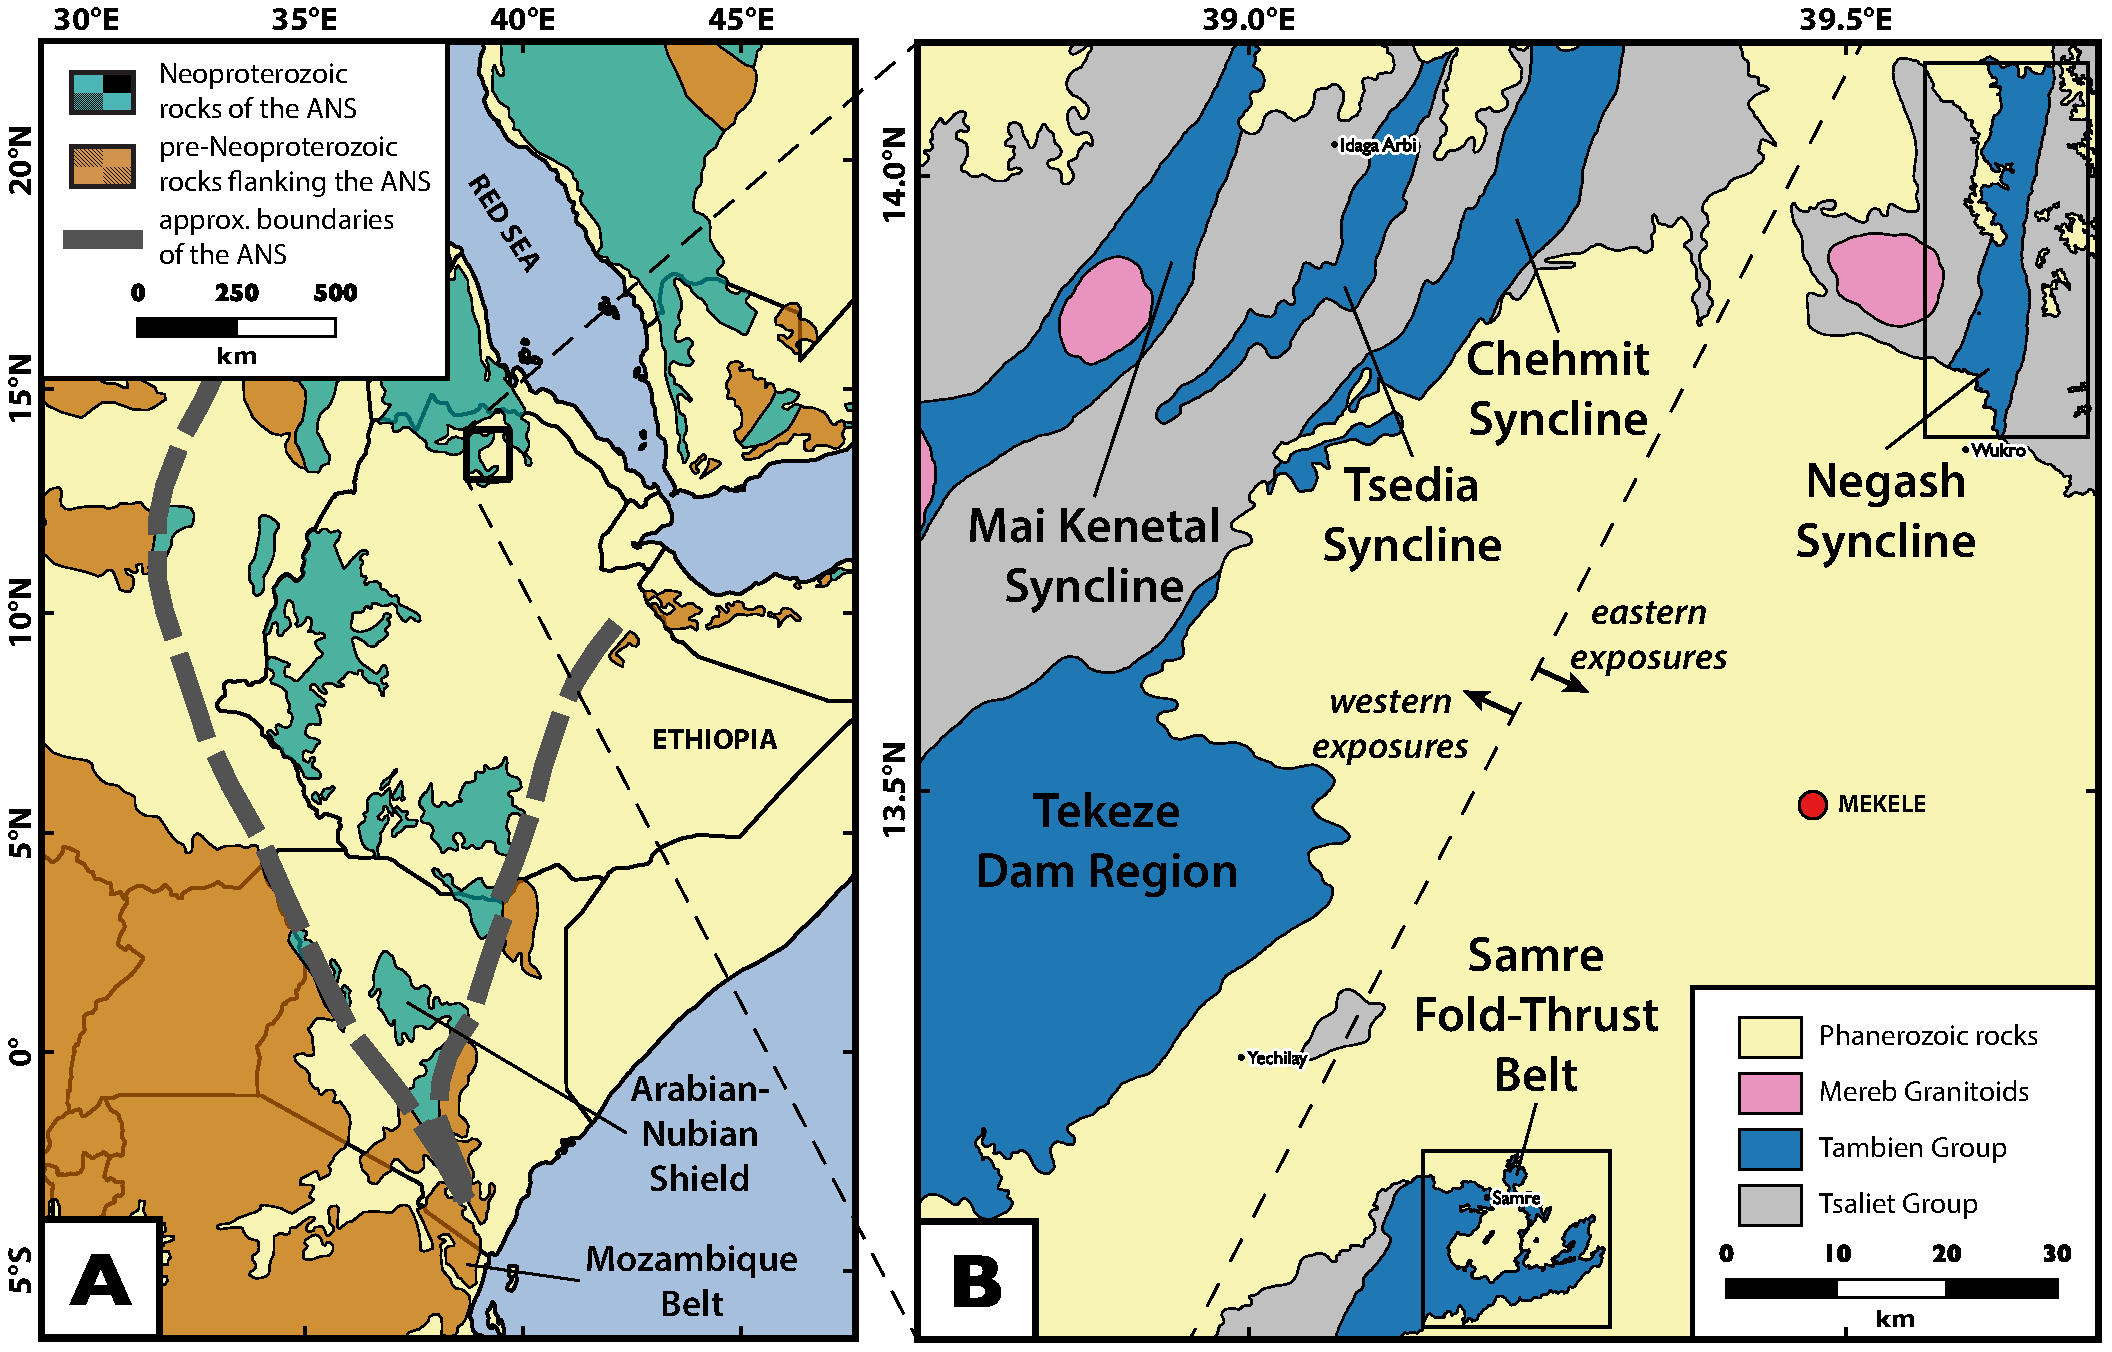
\includegraphics[width=\textwidth]{figures/Tambien/overview-map.pdf}
	\caption[Overview geologic map of the Arabian-Nubian Shield.]{\textbf{A)} Overview geologic map of exposures of the Arabian-Nubian Shield (ANS) and adjacent Archean rocks (simplified from \citealp{Johnson2014a}). \textbf{B)} Overview geologic map of Tambien Group exposures in northern Ethiopia. Inset boxes show the locations of detailed geological maps of the Negash Syncline and Samre Fold-Thrust Belt (Fig. \ref{fig:Negash-Samre-maps}), where sedimentary rocks interpreted to be glacigenic of the Negash Formation have been identified. The dashed line separates what we define as the western and eastern Neoproterozoic exposures in this study.}
	\label{fig:overview-map}
\end{center}
\end{figure}

\begin{figure}[h!]
\begin{center}
	\includegraphics[width=\textwidth]{figures/Tambien/Negash-Samre-maps.pdf}
	\caption[Geologic maps of the upper Tambien Group.]{Geologic maps of the upper Tambien Group corresponding to inset boxes in Figure \ref{fig:overview-map}. \textbf{A)} Negash Syncline geologic map synthesized from \citet{Beyth2003a} and new mapping. \textbf{B)} Samre Fold-Thrust Belt geologic map based on new mapping. There are notable differences in lithostratigraphy across the major NE-striking thrust fault, which we refer to as the Zamra Fault.}
	\label{fig:Negash-Samre-maps}
\end{center}
\end{figure}

\begin{figure}[!htbp]
\begin{center}
	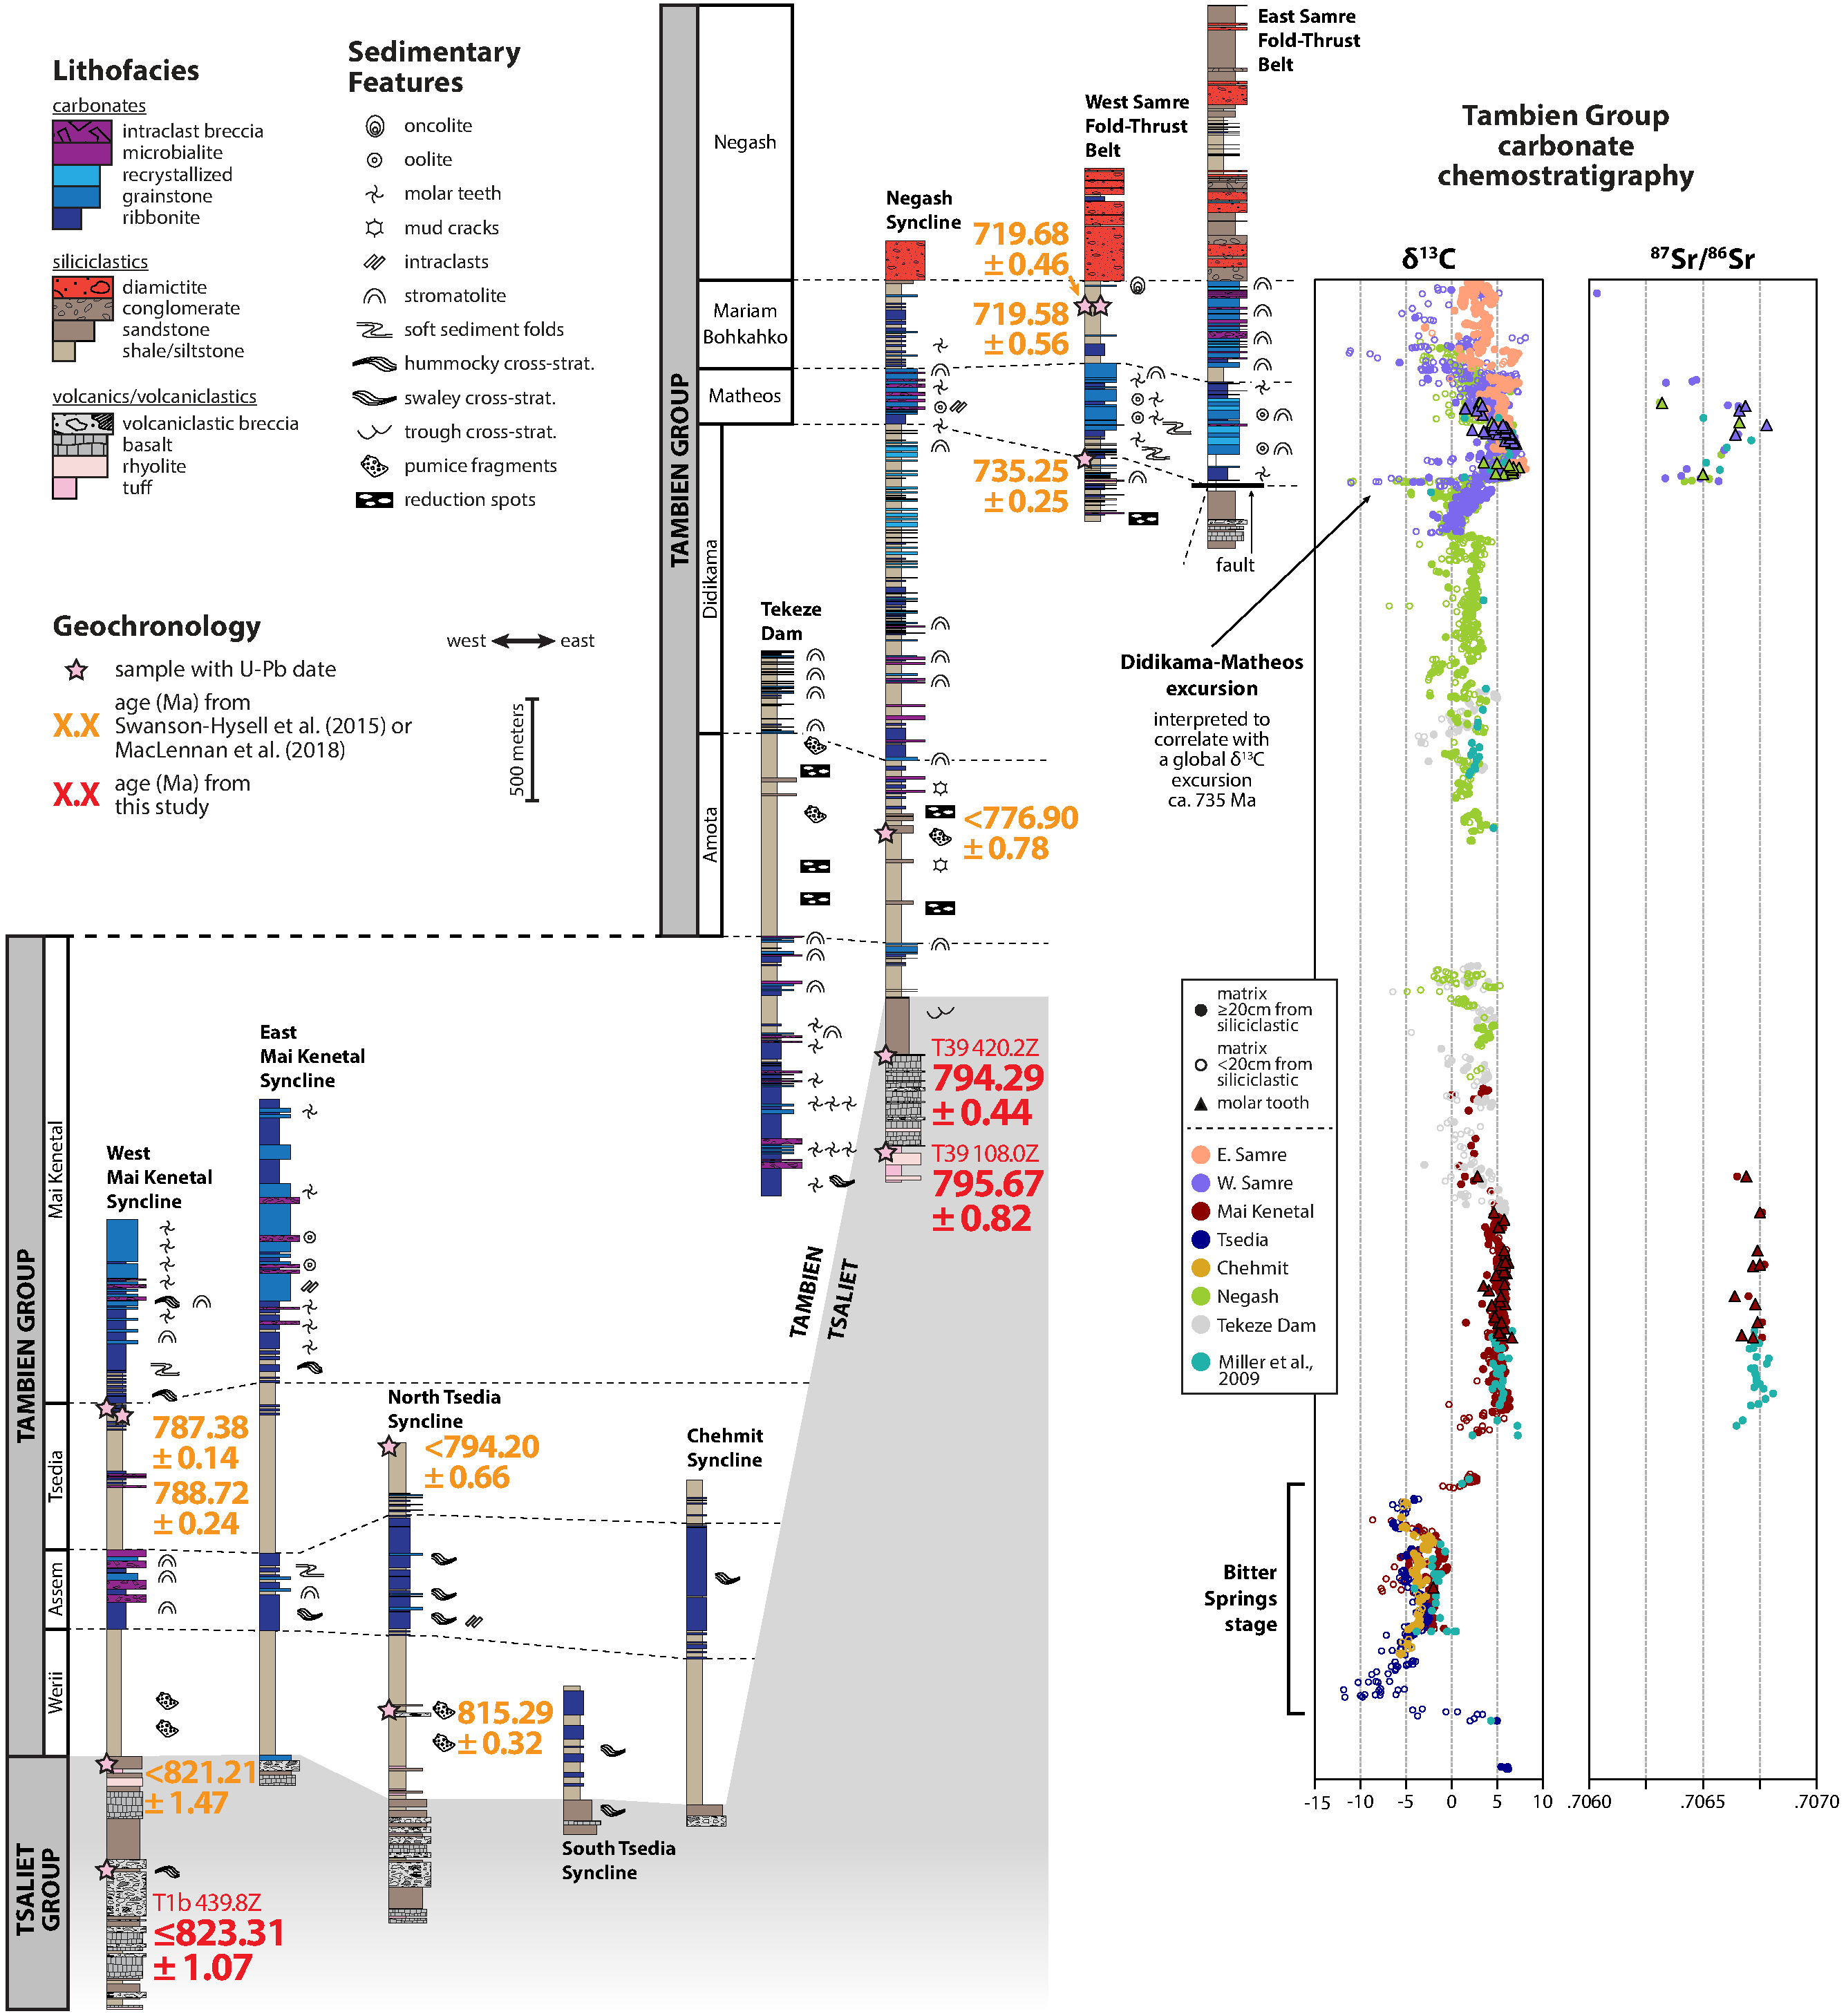
\includegraphics[width=0.95\textwidth]{figures/Tambien/fence-diagram.pdf}
	\caption[Stratigraphy and \dC and \SrSr chemostratigraphy of the Tambien Group.]{Representative simplified stratigraphy and \dC and \SrSr chemostratigraphy of the Tambien Group. For the \dC chemostratigraphy, open circles denote samples that are \textless20~cm from the closest siliciclastic unit. Data from the Tsedia Syncline resolve the onset of the Bitter Springs stage in Ethiopia, and data from the Samre Fold-Thrust Belt and the Negash Syncline resolve the recovery from the nadir of a large negative \dC excursion (the Didikama-Matheos excursion, detailed in Fig. \ref{fig:Didikama-Matheos-sections}). U-Pb ID-TIMS dates are in units of Ma with uncertainties corresponding to the analytical uncertainty, which can be used for comparison between these dates since they were developed using the same tracer. Orange dates are from \citet{Swanson-Hysell2015a} or \citet{MacLennan2018a}, and red dates are from this study. These dates show that the transition from the volcanism of the Tsaliet Group to the sedimentation of the Tambien Group occurred significantly later in the Negash Syncline than in exposures further to the west.}
	\label{fig:fence-diagram}
\end{center}
\end{figure}

The Arabian-Nubian Shield is a region of Neoproterozoic juvenile crust with an area of $\sim$2.7$\times$10$^{6}$~km$^{2}$ that makes up the northern portion of the East African Orogen (Fig. \ref{fig:overview-map}; \citealp{Johnson2014a}). Its construction began with arc and back-arc volcanism generating juvenile crust starting at ca. 858 $\pm$ 7~Ma (sensitive high-resolution ion microprobe (SHRIMP) U-Pb date on zircons from a gneiss of oceanic arc affinity; \citealp{Kuster2008a}) and continuing through the Tonian into the Cryogenian until final terrane accretion in the Ediacaran at ca. 620~Ma (closure of basin constrained by inductively coupled plasma mass spectrometry (ICP-MS) U-Pb dates on detrital zircons and felsic magmatism intruding ophiolites; \citealp{Cox2012a, Johnson2014a, Cox2018a}). The paleogeographic setting in which arc volcanism began is poorly constrained, although it has been proposed that the ocean basin in which this volcanism occurred (known as the Mozambique Ocean) formed as the result of rifting between the Indian, Saharan, and Congo-Tanzanian cratons \citep{Johnson2011a}. However, it is well constrained that this juvenile crust amalgamated as East Gondwana (Indian craton) and West Gondwana (Saharan and Congo-Tanzanian cratons) collided in the Ediacaran resulting in the East African Orogeny \citep{Stern1994a, Fritz2013a}.

The East African Orogeny spanned over 6000~km from the Middle East to Madagascar \citep{Collins2002a, Johnson2014a}. In general, metamorphic grade in the Arabian-Nubian Shield increases from sub-greenschist and greenschist facies in the north to granulite facies in the south, where the Arabian-Nubian Shield transitions into higher grade metamorphic rocks of continental affinity known as the Mozambique Belt (Fig. \ref{fig:overview-map}; \citealp{Johnson2011a}). This overall northward decrease in metamorphic grade allows for the preservation of primary sedimentary structures and geochemical signals in the Arabian-Nubian Shield. As a result, sedimentary rocks in this area are a viable target for reconstructing surface processes and environments at the time of deposition.

The Tambien Group (Fig. \ref{fig:overview-map}) is a Tonian-Cryogenian (ca. 820-700~Ma) sequence of carbonate and siliciclastic sedimentary rocks that culminates in a diamictite that has been interpreted to correlate with the ca. 717-660~Ma Sturtian Glaciation \citep{Beyth2003a, Alene2006a, Miller2009a, Swanson-Hysell2015a, MacLennan2018a}. This sequence was deposited on top of the Tsaliet Group, which consists of volcanic and volcaniclastic lithologies correlated with 854 $\pm$ 3~Ma Eritrean volcanics (Pb-Pb evaporation date; \citealp{Teklay1997a}) that are associated with Arabian-Nubian Shield island arc volcanism. A maximum depositional age near the top of the Tsaliet Group (within 75~m of the Tsaliet-Tambien group contact) of 821.2 $\pm$ 1.5~Ma, and an eruptive age near the base of the Tambien Group ($\sim$150~m above the Tsaliet-Tambien group contact) of 815.29 $\pm$ 0.32~Ma (U-Pb ID-TIMS on zircon; \citealp{Swanson-Hysell2015a}) constrains the age of the Tsaliet-Tambien group transition in the west (Fig. \ref{fig:fence-diagram}). U-Pb ID-TIMS dates of 719.58 $\pm$ 0.56 and 719.68 $\pm$ 0.46~Ma from tuffs $\sim$80~m below the Negash Formation glacial deposits provide the best available maximum age constraints on those deposits and are consistent with a ca. 717 Ma onset of glaciation in the basin (Fig. \ref{fig:fence-diagram}; \citealp{MacLennan2018a}). The strata subsequently were folded into a series of synclines with fold axes oriented NNE-SSW (Fig. \ref{fig:overview-map}B) during the East African Orogeny \citep{Stern1994a}, with maximum metamorphic temperatures estimated to have reached \textless250\degreesC based on chlorite thermometry \citep{Alene1998a}. Synchronous with and following this deformation was the emplacement of granitoid plutons, known as the Mereb Granitoids, into the Tambien Group (Fig. \ref{fig:overview-map}) with dates of ca. 610~Ma (U-Pb SHRIMP and Pb-Pb evaporation; \citealp{Miller2003a, Avigad2007a}).

\section{Methods}

\subsection{Field Methods}

Tambien Group rocks near the town of Samre in the Tigray region of northern Ethiopia previously were mapped as `undifferentiated Neoproterozoic sedimentary rocks' \citep{Arkin1971a}, and no Neoproterozoic diamictite from the region was reported in the literature, with the notable exception of a brief mention in \citet{Bussert2010a}. Our geologic mapping of this area has revealed extensive exposures of upper Tambien Group strata including large areas of diamictite within a series of folds (Fig. \ref{fig:Negash-Samre-maps}). We refer to this area as the Samre Fold-Thrust Belt, and differentiate units within it based on the stratigraphic framework developed in the Negash Syncline \citep{Swanson-Hysell2015a} since the lithostratigraphy of the strata correlates well between the two areas (Fig. \ref{fig:fence-diagram}). Stratigraphic sections with good exposure were identified and measured using a Jacob's staff in both the Negash Syncline and the Samre Fold-Thrust Belt. During the measurement of these sections, carbonate samples with minimal visible alteration were collected for geochemical analyses at a resolution of $\sim$0.5-5~m (depending on proximity to other measured sections) where the stratigraphy is carbonate dominated, and wherever possible where the stratigraphy is siliciclastic dominated.

\subsection{Geochemical Analyses}

Carbonate samples were cut perpendicular to bedding to expose a fresh surface before micro-drilling. Visibly altered zones of the fresh surface, such as those exhibiting veins and/or fractures, were avoided. The subsequent analyses described here were performed on aliquots of these micro-drilled powders.

\begin{figure}[h!]
\begin{center}
	\includegraphics[width=\textwidth]{figures/Tambien/MTS-petrography.pdf}
	\caption[Molar tooth structures from the Tambien Group.]{Molar tooth structures from the Tambien Group. \textbf{A)} and \textbf{B)} Photographs in cross-section view of molar tooth structures from the Mai Kenetal Formation, showing differential compaction of carbonate ribbonite around the structures. The 10 cent of Ethiopian birr coin used for scale has a diameter of 23~mm. \textbf{C)} Photomicrograph in cross-section view of molar tooth structures within ribbonite of the Mariam Bohkahko Formation from the Negash Syncline taken using cross-polarized light. Inset box shows field of analysis for D. \textbf{D)} Wavelength-dispersive x-ray spectroscopy elemental maps of a molar tooth structure, with warmer colours indicating higher concentration. The maps show the high purity of the microspar calcite in the molar tooth structures relative to the surrounding micrite matrix. Low Mg and high Ca suggests undolomitized calcite, and low Fe suggests a lack of a clay component or Fe-rich carbonate.}
	\label{fig:MTS-petrography}
\end{center}
\end{figure}

Previous work has determined that molar tooth structures typically consist of high purity microspar calcite relative to the surrounding micrite host \citep{Smith1968a, Fairchild1997a, Pratt1998a}. These structures appear as subvertical dual-tapered carbonate-cement-filled cracks that are generally \textless1~cm wide, and historically their plan view was interpreted to resemble the upper surface of elephant molar teeth (Fig. \ref{fig:MTS-petrography}; \citealp{Bauerman1884a, Daly1912a}). The differential compaction of sediment around molar tooth structures, which typically are crumpled perpendicular to bedding planes, requires that molar tooth structures formed prior to or during compaction and dewatering of the sediment. Hypotheses of molar tooth structure crack formation are varied and include subaqueous shrinkage cracks \citep{Smith1968a}, the expansion of gas from organic decay \citep{Pollock2006a}, wave-induced cracking due to heaving of sediment \citep{Bishop2006a}, or microbial conversion of smectite to illite coupled with wave loading \citep{Hodgskiss2018a}. Regardless of the mode of crack formation, precipitation of calcite cement within the cracks requires significant throughput of seawater prior to or during dewatering and lithification of the host carbonate mud.

Molar tooth structures occur in a number of formations in the Tambien Group (Fig. \ref{fig:fence-diagram}), often in ribbonite (thinly bedded wavy- to parallel-laminated fine-grained limestone) that can exhibit swaley cross-stratification. Petrographic analysis shows that these structures consist of high purity calcite microspar, whereas the surrounding micrite can have a clay component (Fig. \ref{fig:MTS-petrography}). Furthermore, in samples where the surrounding micrite is partially dolomitized, molar tooth structures are not (Fig. \ref{fig:MTS-petrography}), suggesting that the structures are more resistant to dolomitization. Therefore, wherever possible, molar tooth structure microspar calcite was targeted for geochemical analyses along with the host bulk carbonate matrix.

\subsubsection{\dC and \dO}

Carbonate powders were weighed out to 1~mg and heated to 110\degreesC to remove any residual water. Samples then were reacted with 250~$\mu$L of H$_{3}$PO$_{4}$ at 75\degreesC. The resulting CO$_{2}$ gas was extracted using a GasBench II auto-sampler and analyzed on a SerCon Callisto continuous-flow isotope ratio mass spectrometry (CF-IRMS) system at Princeton University to obtain \dC and \dO values. Powders of NBS-19 (\dC = 1.95\permil and \dO = -2.20\permil) and an internally calibrated standard (\dC = -1.48 $\pm$ 0.1\permil and \dO = -8.54 $\pm$ 0.1\permil) also were analyzed once every 10 samples to calibrate the sample measurements. Typical measured precision was $\sigma$ = 0.1\permil for \dC and $\sigma$ = 0.2\permil for \dO.

\subsubsection{Elemental Analysis}

Carbonate powders were weighed out to 10~mg and then reacted with 10.0~mL of pH = 4.9 buffered acetic acid solution (3~mL of glacial acetic acid and 3~mL of ammonium hydroxide for every 497~mL of water) for 4-5 hours in a 25\degreesC sonicator. Samples then were centrifuged, and 0.8~mL of the solution was extracted and mixed with 7.2~mL of 2\% HNO$_{3}$. These diluted samples were simultaneously analyzed for Al, Ca, Fe, Mg, Mn, K, Na, and Sr on a Perkin Elmer 5300 DV inductively coupled plasma optical emission spectrometer (ICP-OES) in the College of Natural Resources at UC Berkeley. Raw measurements were transformed into concentrations using 6 internal standards of known concentration with 2\% HNO$_{3}$ matrix (diluted from a commercial standard of known concentration). Standard concentrations bracketed the concentrations observed in samples. When the known concentrations were plotted against measured intensity, linear fits through these 6 standards produced R$^{2}$\textgreater0.98 for Al and K, R$^{2}$\textgreater0.999 for Ca, Mg, and Na, and R$^{2}$\textgreater0.9999 for Fe, Mn, and Sr.

\subsubsection{\SrSr}

Carbonate powders were weighed out to $\sim$30~mg and washed 3 times in a 1.0~mL 1:1 methanol:water solution to encourage the suspension of clays \citep{McArthur2006a}. The samples then were reacted in an ultrasonic bath 3 times with 1.0~mL of 0.2~M ammonium acetate to remove loosely bound Sr cations and rinsed in an ultrasonic bath 3 times with ultrapure water to remove residual ammonium and clay. These cleaned samples then were reacted with 1.0~mL of 0.5~M acetic acid, and any insoluble residue was removed via a centrifuge. The sample solutions then were dried down using heating lamps in a nitrogen atmosphere and then reacted with 250~$\mu$L of 6~M HNO$_{3}$. Sr was isolated via standard column chemistry techniques using 100-150~$\mu$m Sr-spec resin, dried down again with 3 drops of 15~M HNO$_{3}$, and then loaded onto single rhenium filaments in H$_{3}$PO$_{4}$ with a TaCl$_{5}$ activator. Strontium isotopes were measured on a ThermoFisher Triton thermal ionization mass spectrometer (TIMS) at the Center for Isotope Geochemistry at UC Berkeley using a static multicollection routine. Mass discrimination was corrected to $^{86}$Sr/$^{88}$Sr = 0.11940. A minor correction ratio of \textless1.00003 also was applied to the raw data to match the \SrSr of blanks with NBS-987 (\SrSr = 0.710245), which was analyzed alongside the samples.

\subsubsection{U-Pb Geochronology}

\begin{sidewaystable*}[!htbp]

\scriptsize
\caption[CA-ID-TIMS \UPb dates from the Tsaliet and Tambien groups.]{Summary of CA-ID-TIMS \UPb dates from the Tsaliet and Tambien groups.}
\vspace{0.2cm}
\resizebox{\linewidth}{!}{
\begin{tabular}{llllll}
& \textbf{Description and} & \textbf{Latitude} & \textbf{\UPb} & & \\
\textbf{Sample} & \textbf{Formation/Group}  & \textbf{Longitude} & \textbf{Date (Ma)} & \textbf{Type} & \textbf{Reference} \\
\hline
&&&&& \\
T1-12.3 & volcaniclastic unit & 14.0444\textdegree N & \textless821.2 & maximum depositional age from & \citealp{Swanson-Hysell2015a} \\
& upper Tsaliet Grp. & 38.9554\textdegree E & $\pm$1.5 & youngest concordant single crystal & \\
&&&&& \\
TS22 & tuff & 14.0382\textdegree N & 815.29 & eruptive age from weighted mean & \citealp{Swanson-Hysell2015a} \\
& Werii Fm. & 39.1079\textdegree E & $\pm$0.32/0.46/0.99 & (MSWD=0.52, n=5) & \\
&&&&& \\
TS23 & siltstone & 14.0379\textdegree N & \textless794.20 & maximum depositional age from & \citealp{Swanson-Hysell2015a} \\
& Tsedia Fm. & 39.1298\textdegree E & $\pm$0.66 & youngest concordant single crystal & \\
&&&&& \\
T2 & tuff & 14.0437\textdegree N & 788.72 & eruptive age from weighted mean & \citealp{Swanson-Hysell2015a} \\
& upper Tsedia Fm. & 38.9733\textdegree E & $\pm$0.24/0.40/0.94 & (MSWD=1.2, n=6) & \\
&&&&& \\
T1-1202 & tuff & 14.0482\textdegree N & 787.38 & eruptive age from weighted mean & \citealp{Swanson-Hysell2015a} \\
& upper Tsedia Fm. & 38.9757\textdegree E & $\pm$0.14/0.35/0.91 & (MSWD=18, n=7) & \\
&&&&& \\
T22-453 & volcaniclastic unit & 13.8436\textdegree N & \textless776.90 & maximum depositional age from & \citealp{Swanson-Hysell2015a} \\
& Amota Fm. & 39.6397\textdegree E & $\pm$0.78 & youngest concordant single crystal & \\
&&&&& \\
T46-102.2Z & tuff & 13.1588\textdegree N & 735.35 & eruptive age from weighted mean & \citealp{MacLennan2018a} \\
& lower Matheos Fm. & 39.2512\textdegree E & $\pm$0.25/0.39/0.88 & (MSWD=0.36, n=5) & \\
&&&&& \\
SAM-ET-04 & tuff & 13.1398\textdegree N & 719.68 & eruptive age from weighted mean & \citealp{MacLennan2018a} \\
& upper Mariam Bohkahko Fm. & 39.1763\textdegree E & $\pm$0.46/0.54/0.94 & (MSWD=1.3, n=8) & \\
&&&&& \\
SAM-ET-03 & tuff & 13.1398\textdegree N & 719.58 & eruptive age from weighted mean & \citealp{MacLennan2018a} \\
& upper Mariam Bohkahko Fm. & 39.1761\textdegree E & $\pm$0.56/0.64/1.0 & (MSWD=0.54, n=3) & \\
&&&&& \\
T1b-439.8Z & lava flow & 14.0445\textdegree N & \textless823.3 & maximum eruptive age from & this study \\
& Tsaliet Grp. & 38.9522\textdegree E & $\pm$1.1 & youngest concordant single crystal & \\
&&&&& \\
T39-108.0Z & ignimbrite & 13.8488\textdegree N & 795.67 & eruptive age from weighted mean & this study \\
& Tsaliet Grp. & 39.6523\textdegree E & $\pm$0.82/0.89/1.2 & (MSWD=0.084, n=3) & \\
&&&&& \\
T39-420.2Z & tuff & 13.8509\textdegree N & 794.29 & eruptive age from weighted mean & this study \\
& Sa'aga Fm. of the Tsaliet Grp. & 39.6499\textdegree E & $\pm$0.44/0.51/0.99 & (MSWD=0.21, n=5) & \\
&&&&& \\
\hline
\end{tabular}}

\begin{tablenotes}[para, flushleft]
\emph{Notes:} \\
2$\sigma$ uncertainties are reported in the format  $\pm$ X/Y/Z, where X is the internal (analytical) uncertainty in the absence of all external or systematic errors, Y is the uncertainty incorporating the U-Pb tracer calibration error, and Z is the uncertainty including X and Y, as well as the uranium decay constant uncertainty; MSWD = mean square of weighted deviates; n = number of zircon analyses included in the calculated date.
\end{tablenotes}

\label{tab:geochronology}
\end{sidewaystable*}

Zircons were extracted from rock samples at Princeton University by crushing using a jaw crusher and disc mill followed by magnetic and gravimetric separation. The zircon separates were annealed in quartz crucibles at 900\degreesC for 48 to 60 hours. Individual zircons were photographed and transferred to microcapsules, after which 100~$\mu$g of 29~M HF and 15~$\mu$g of 30\% HNO$_{3}$ were added. The microcapsules were put into a Parr bomb and placed in an oven at 195\degreesC for 12 hours to chemically abrade the zircons, preferentially targeting metamict and damaged parts of the zircon that have undergone Pb loss. After chemical abrasion, the zircon grains were rinsed in ten steps of alternating distilled 6~N HCl, 30\% HNO$_{3}$ and MQ water. Distilled HF and HNO$_{3}$ were again added, as well as the EARTHTIME ET535 tracer solution \citep{Condon2015a, McLean2015a}, before total dissolution at 210\degreesC for 48 hours. After total dissolution, the solutions were dried down and converted to chlorides. U and Pb separation was performed using ion exchange resin (Eichrom 200-400 mesh chloride form).

The U and Pb cut was dried down with a microdrop of dilute H$_{3}$PO$_{4}$. The dried U-Pb fraction was redissolved in a silica gel emitter, and deposited onto outgassed zone-refined Re filaments. U and Pb isotopic measurements were made using an IsotopX PhoeniX-62 TIMS at Princeton University. Pb analyses were performed in peak hopping mode on a Daly photomultiplier ion counting detector. Depending on the signal intensity, U measurements were made either on the Daly photomultiplier in peak hopping mode or as a static measurement on the Faraday cups connected to 10$^{12}$~ohm resistor boards. U was measured as an oxide. The Pb and U deadtime characteristics of the Daly photomultiplier were monitored by running NBS982 and CRM U500 on a weekly basis. The NBS982 runs also were used to quantify Pb mass-dependent fractionation. Unless stated otherwise, all U-Pb uncertainties reported in this manuscript are the internal (analytical) uncertainties in the absence of all external or systematic errors, with these additional uncertainties reported in Table \ref{tab:geochronology}.

\section{Lithostratigraphy}

From oldest to youngest, nine formations within the Tambien Group have been differentiated: the Werii, Assem, Tsedia, Mai Kenetal, Amota, Didikama, Matheos, Mariam Bohkahko, and Negash formations (Figs. \ref{fig:Negash-Samre-maps} and \ref{fig:fence-diagram}; \citealp{Swanson-Hysell2015a}). In the Negash Syncline, the Negash Formation is limited in aerial extent to $\sim$3~km$^{2}$ and is more penetratively foliated than most of the Tambien Group since it is only exposed in the southern-most core of the syncline (Fig. \ref{fig:Negash-Samre-maps}). Our team's mapping now has differentiated extensive exposures of the Negash Formation, along with further exposures of the underlying strata, in the Samre Fold-Thrust Belt (Figs. \ref{fig:overview-map} and \ref{fig:Negash-Samre-maps}).

\begin{figure}[h!]
\begin{center}
	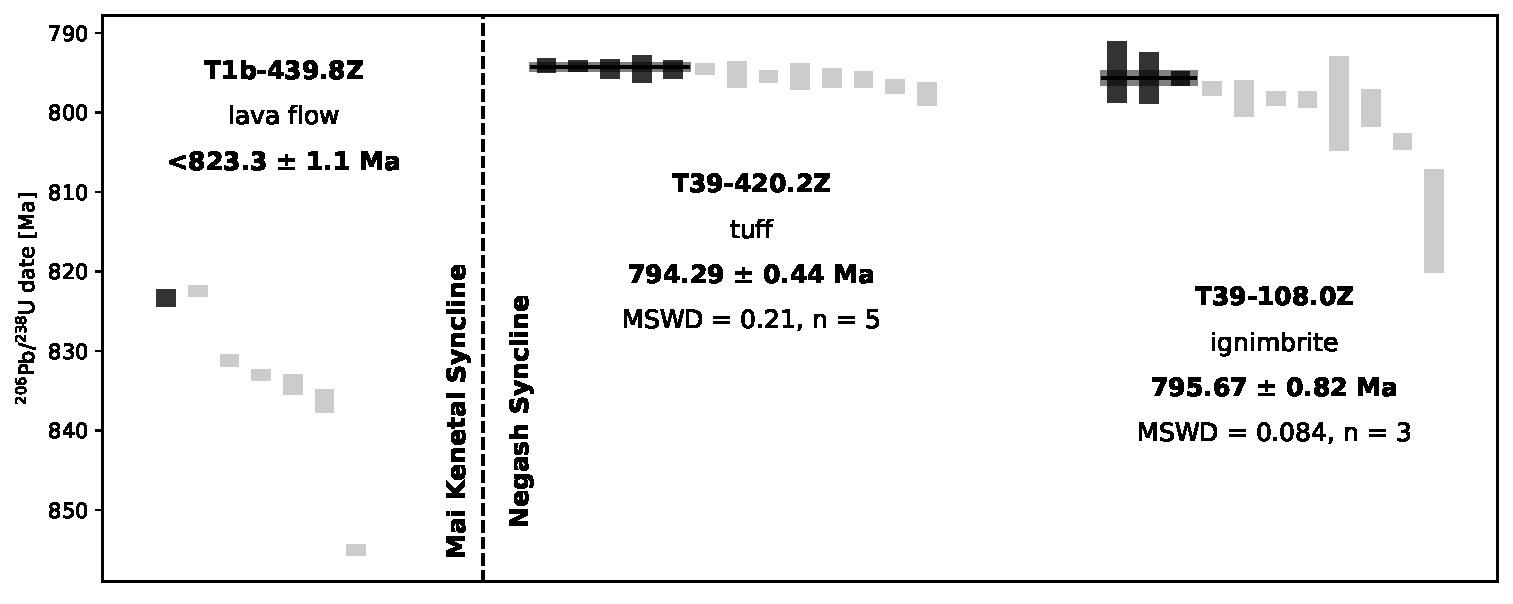
\includegraphics[width=0.9\textwidth]{figures/Tambien/geochronology.pdf}
	\caption[U-Pb ID-TIMS analyses for individual zircon grains.]{U-Pb ID-TIMS analyses for individual zircon grains. T1b-439.8Z is from the Tsaliet Group in the Mai Kenetal Syncline, and T39-420.2Z and T39-108.0Z are from the Tsaliet Group in the Negash Syncline (Fig. \ref{fig:fence-diagram}). Vertical bars represent the 2$\sigma$ uncertainty for the \UPb date of each zircon. Black vertical bars represent zircons included in the calculation of the weighted mean. Reversely discordant zircons are not shown. Horizontal lines and grey bars represent the calculated weighted means and 2$\sigma$ uncertainties respectively. MSWD = mean square of weighted deviates; n = number of zircon analyses included in the calculated date. Concordia diagrams, data tables, and sample photos are included in the \SI.}
	\label{fig:geochronology}
\end{center}
\end{figure}

\begin{figure}[!htbp]
\begin{center}
	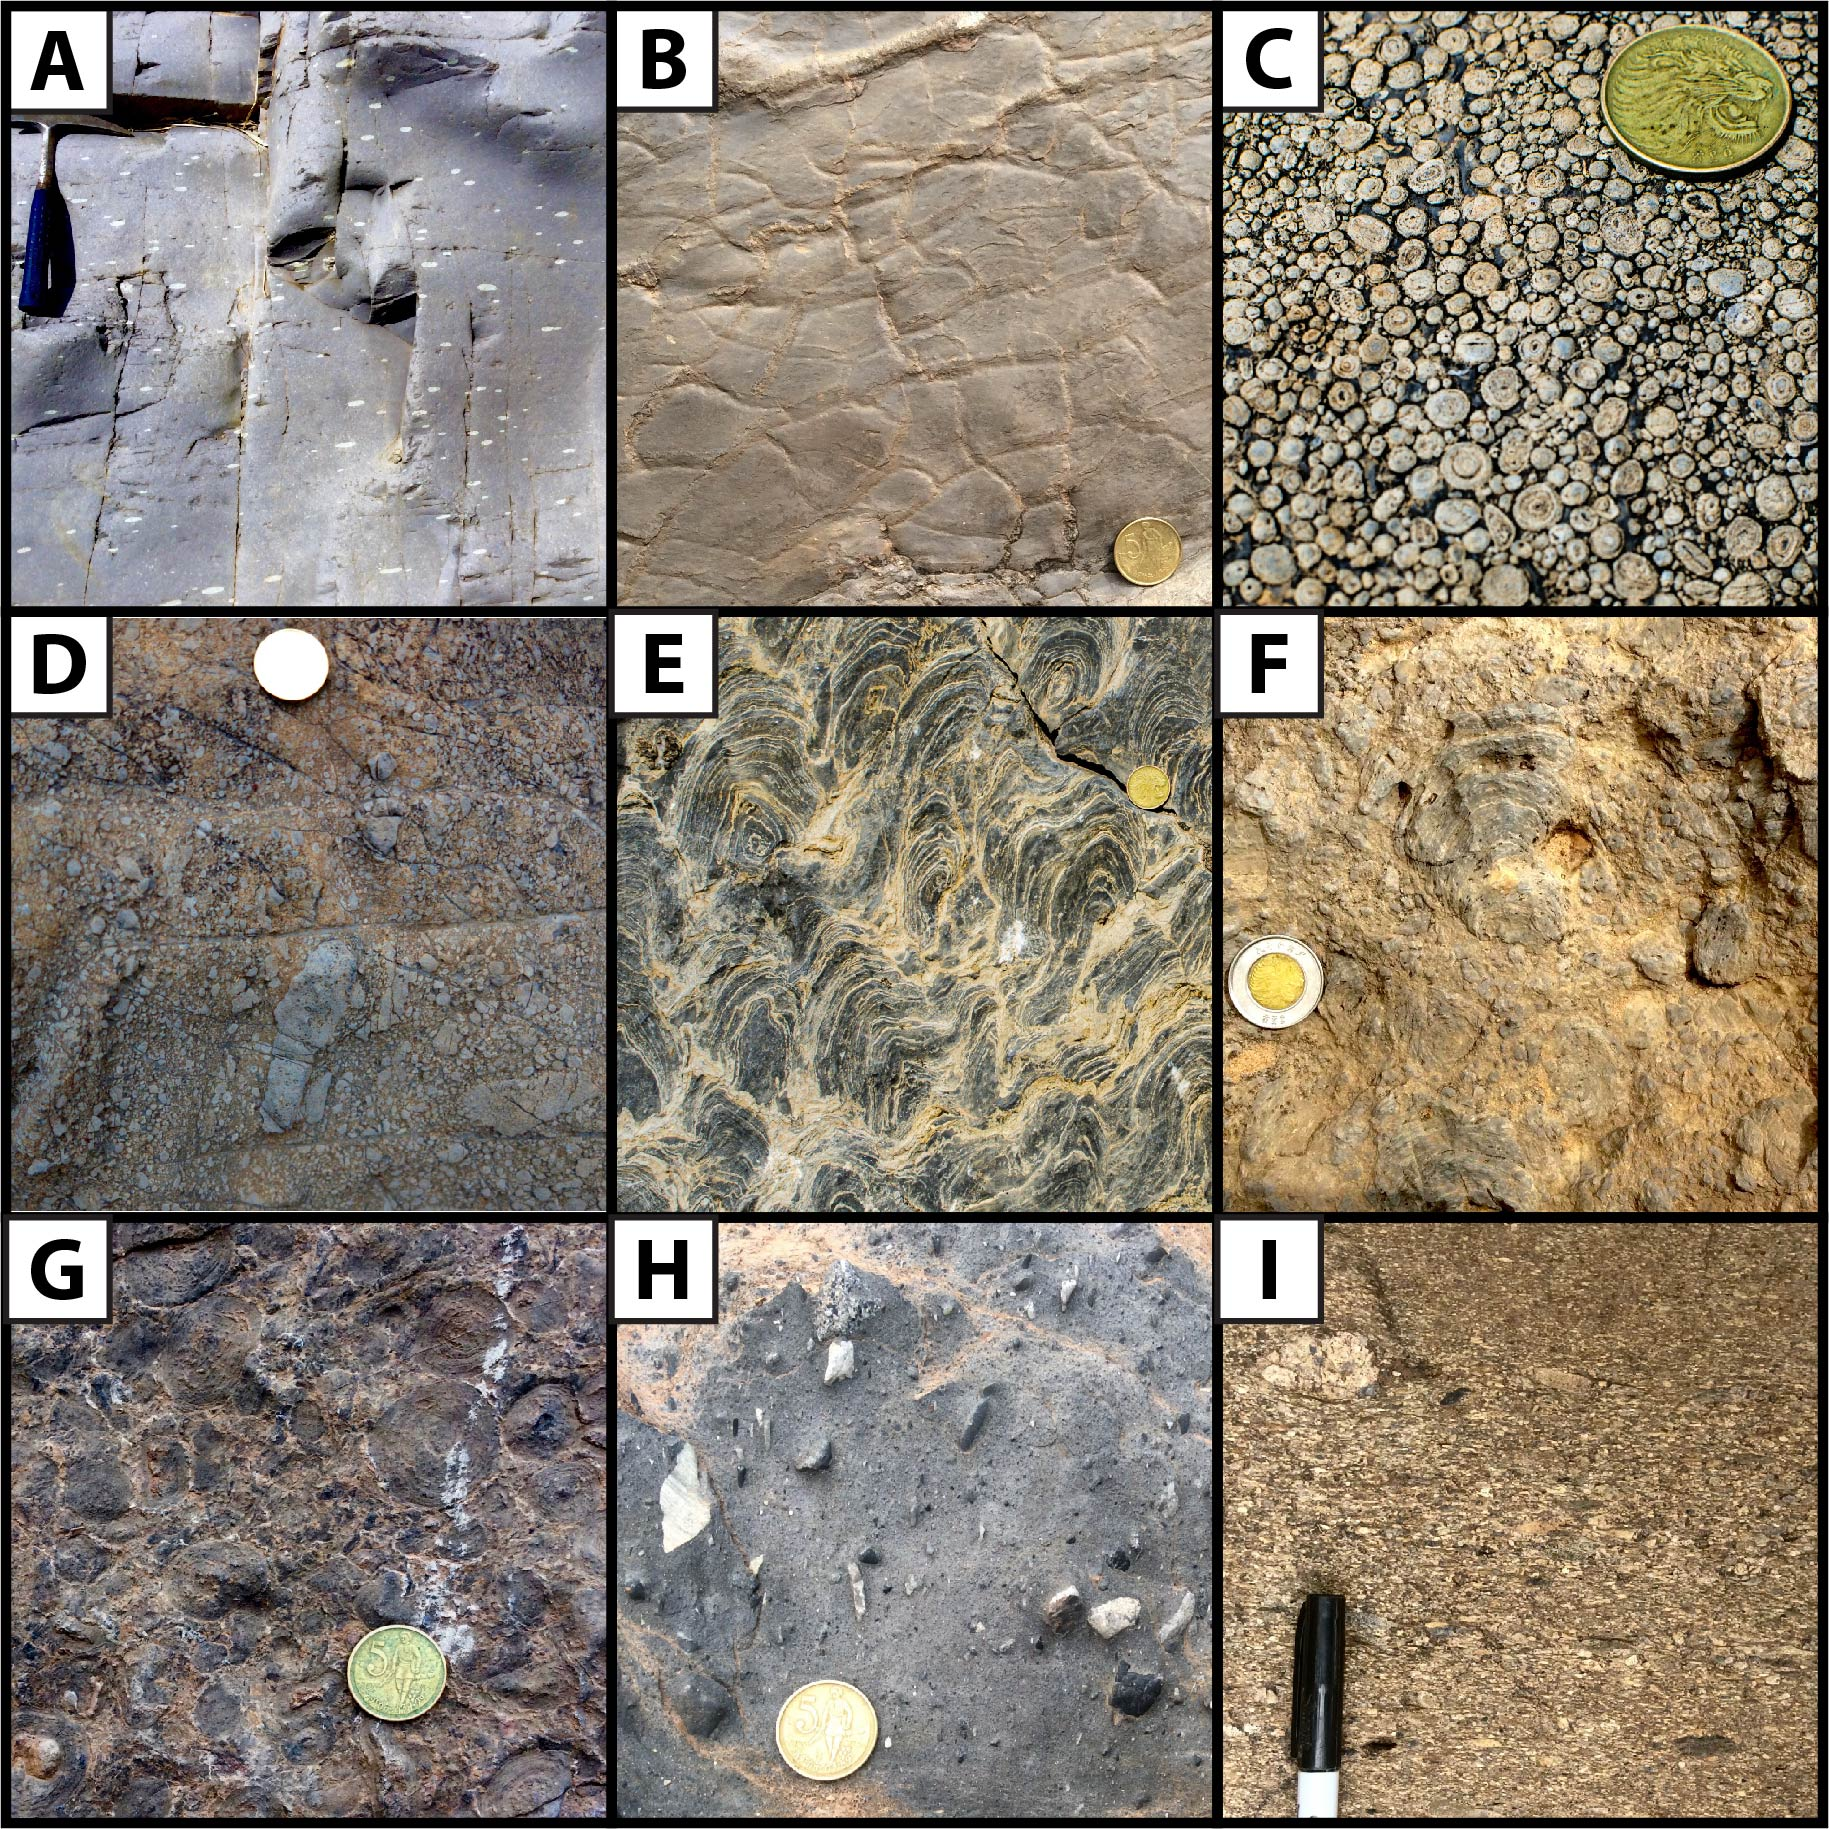
\includegraphics[width=0.9\textwidth]{figures/Tambien/lithofacies.jpg}
	\caption[Photos of key lithofacies of the Tambien Group.]{Photos of key lithofacies of the Tambien Group. \textbf{A)} Reduction spots within siltstones of the Amota Formation in the Negash Syncline. \textbf{B)} Mud cracks within siltstones of the Amota Formation in the Negash Syncline. \textbf{C)} Oolite within the Matheos Formation in the Samre Fold-Thrust Belt. \textbf{D)} Limestone intraclast breccia within the Matheos Formation in the Samre Fold-Thrust Belt. \textbf{E)} Stromatolites at the base of the Mariam Bohkahko Formation in the western Samre Fold-Thrust Belt. \textbf{F)} Carbonate breccia containing stromatolites from the Mariam Bohkahko Formation in the eastern Samre Fold-Thrust Belt. \textbf{G)} Oncolite from near the top of the Mariam Bohkahko Formation in the Samre Fold-Thrust Belt. \textbf{H)} Diamictite of the Negash Formation in the Samre Fold-Thrust Belt. \textbf{I)} Lithic arkose coarse sandstone with sparse pebbles of the Negash Formation in the Samre Fold-Thrust Belt. The hammer used for scale in A has a length of 33~cm. The 5 cent of Ethiopian birr coin used for scale in B, C, D, E, G and H has a diameter of 20~mm. The 1 Ethiopian birr coin used for scale in F has a diameter of 27~mm. The pen used for scale in I has a width of 1~cm. All photos are in cross-section views except B, which is of a bedding plane.}
	\label{fig:lithofacies}
\end{center}
\end{figure}

\subsection{Western Exposures}

In broad terms, mapping of the Tambien Group to date has revealed that older formations are exposed in the western synclines and younger formations are exposed in the eastern synclines, with the Tekeze Dam Region in the southwest exposing stratigraphy that links the two areas (\citealp{Swanson-Hysell2015a}, building upon the work of \citealp{Beyth1972a}, \citealp{Hailu1975a}, and \citealp{Garland1980a}). We define western Neoproterozoic exposures as the Mai Kenetal Syncline, Tsedia Syncline, Chehmit Syncline, and Tekeze Dam Region (Fig. \ref{fig:overview-map}). Lithostratigraphic correlation between these four areas is relatively straightforward, although there is notable lateral variability (Fig. \ref{fig:fence-diagram}). The lithostratigraphic framework of these western exposures, as well as \dC and geochronologic data from these areas, were developed by \citet{Swanson-Hysell2015a}. This study adds to this previous work by describing in detail the lithostratigraphy of the western exposures, adding an age constraint to the upper Tsaliet Group in the Mai Kenetal Syncline, developing new \dC data from previously unreported limestone ribbonite horizons within the Werii Formation in the southwestern Tsedia Syncline, and developing new \SrSr data from the Mai Kenetal Formation (Fig. \ref{fig:fence-diagram}). These \SrSr data add to those developed in \citet{Miller2009a}.

\subsubsection{Tsaliet Group}

The Tsaliet Group comprises basaltic to intermediate lava flows, volcaniclastic breccias, and ignimbrites (Fig. \ref{fig:fence-diagram}). The lava flows can have vesiculated flow tops and are sometimes porphyritic with cm-scale tabular plagioclase phenocrysts. The volcaniclastic breccias have clasts as large as boulders and dominate portions of the group where there are few flows. The presence of flows and the ubiquity of large volcanic clasts in the breccias suggest that deposition of the Tsaliet Group would have happened on, or adjacent to, an active arc.

A maximum depositional age of 821.2 $\pm$ 1.5~Ma (youngest concordant zircon U-Pb ID-TIMS date) from a volcaniclastic unit in the Mai Kenetal Syncline within 75~m of the top of the Tsaliet Group \citep{Swanson-Hysell2015a} was the best available constraint on the start of Tambien Group deposition. In this study, we report a U-Pb ID-TIMS date of 823.3 $\pm$ 1.1~Ma from the youngest concordant zircon grain analyzed within a lava flow $\sim$250~m below the top of the Tsaliet Group of the western limb of the Mai Kenetal Syncline. This result constrains the flow to be this age or younger, since no consistent age population of multiple zircons was identified in the analyzed sample (Figs. \ref{fig:fence-diagram} and \ref{fig:geochronology}; Table \ref{tab:geochronology}).

\subsubsection{Werii Formation}

The Werii Formation is a $\sim$400-500~m thick sequence of siltstones and very fine sandstones exposed in the Mai Kenetal, Chehmit, and Tsedia synclines, except in the southwestern Tsedia Syncline where previously unreported limestone ribbonite horizons are interbedded within siltstones (Fig. \ref{fig:fence-diagram}). The transition from the Tsaliet Group to the Werii Formation appears conformable where observed with decreasing volcaniclastics up stratigraphy. An eruptive U-Pb ID-TIMS age of 815.29 $\pm$ 0.32~Ma from a welded volcanic tuff with pumice fragments 150~m above the base of the Werii Formation in the Tsedia Syncline \citep{Swanson-Hysell2015a} is consistent with this interpretation of conformable deposition when compared to the age constraints within the upper Tsaliet Group.

The strata contains large (up to 50~cm) hyper-vesiculated scoria bombs in the proximity of the tuff that yields the 815.29 $\pm$ 0.32~Ma age. The presence of these bombs indicates that arc volcanism remained nearby and active during the deposition of the Werii Formation, but was more distal than during the deposition of flows and volcaniclastic breccias of the Tsaliet Group.

\subsubsection{Assem Formation}

A transition into carbonate-dominated stratigraphy marks the beginning of the Assem Formation, which is $\sim$200-300~m thick and exposed in the Mai Kenetal, Chehmit, and Tsedia synclines (Fig. \ref{fig:fence-diagram}). There is significant west-east lateral facies variability in the Assem Formation. In the Mai Kenetal Syncline, ribbonite dominates at the base of the formation, and transitions upwards into microbialaminite, stromatolite, and intraclast breccia horizons. This sequence of lithofacies suggests shallowing through the deposition of the Assem Formation such that the upper part of the formation was deposited in a high energy environment within the photic zone. To the east, in the Tsedia and Chehmit synclines, the formation is dominated by ribbonite with swaley cross-stratification likely developed by the combined flow of storm waves. This west-east variability suggests transportation of carbonate mud from a shallow-water microbial carbonate factory in the west out to greater depths to the east.

\subsubsection{Tsedia Formation}

The Tsedia Formation is $\sim$500~m thick and characterized by siltstones interbedded with cm-scale carbonates. The formation is exposed in the Mai Kenetal, Chehmit, and Tsedia synclines, and has a transitional contact with the underlying carbonate-dominated Assem Formation (Fig. \ref{fig:fence-diagram}). The full thickness of the Tsedia Formation only is known to be exposed within the Mai Kenetal Syncline, as the formation is the highest level of the stratigraphy exposed in the other places it has been mapped (Tsedia and Chehmit synclines). However, exposure of the Tsedia Formation is poor throughout the Mai Kenetal Syncline, with the best exposures as it transitions into the overlying Mai Kenetal Formation.

U-Pb ID-TIMS dates within the Tsedia Formation constrain its age: from the Tsedia Syncline there is a maximum depositional age constraint of 794.20 $\pm$ 0.66~Ma from detrital zircons within a siltstone near the base of the formation, and from the Mai Kenetal Syncline there are eruptive ages of 788.72 $\pm$ 0.24 and 787.38 $\pm$ 0.14~Ma \citep{Swanson-Hysell2015a}. These latter two eruptive dates are from tuffs with feldspar phenocrysts $\sim$25~m below the base of the Mai Kenetal Formation.

\subsubsection{Mai Kenetal Formation}

Similar to the Werii-Assem formation contact, the Tsedia-Mai Kenetal formation contact is marked by a transition into the carbonate-dominated stratigraphy of the $\sim$1400~m thick Mai Kenetal Formation. In the western exposures, the formation is exposed in the Mai Kenetal Syncline and Tekeze Dam Region (Fig. \ref{fig:fence-diagram}). The lower part of the formation consists of ribbonite carbonate with abundant hummocky and swaley cross-stratification occasionally interbedded with siltstones, suggesting deposition at intermediate depths that commonly experienced combined waves and currents below fair weather base. These strata transition into a series of \textless10~m thick shallowing-upward parasequences defined by siltstone, ribbonite, grainstone, and intraclast breccia. Well-developed molar tooth structures (Figs. \ref{fig:MTS-petrography} and \ref{fig:lithofacies}) are abundant throughout the formation. This formation represents the youngest rocks of the Tambien Group known to be exposed in the Mai Kenetal Syncline.

\subsubsection{Amota Formation}

The Amota Formation is a $\sim$500~m thick siliciclastic unit exposed in the Tekeze Dam Region and the Negash Syncline of the eastern exposures (Fig. \ref{fig:fence-diagram}). The formation's base is transitional and marked by the last carbonate horizon before hundreds of meters of fine-grained siliciclastic lithofacies. Reduction spots (flattened green ellipsoids $\sim$1-3~cm long) frequently contrast against the purple of the siltstones within this formation (Fig. \ref{fig:lithofacies}). In some cases, the reduction spots are cored with recrystallized minerals, including chlorite, that may have originated as pumice that sank into the depositional environment of the siltstone. In the Tekeze Dam Region, the formation comprises relatively homogenous purple siltstones with rare sandstone interbeds.

\subsubsection{Didikama Formation}

Like the Amota Formation, the only documented exposure of the Didikama Formation in the western exposures is in the Tekeze Dam Region (Fig. \ref{fig:fence-diagram}). The formation represents the highest exposed stratigraphy of the Tambien Group currently recognized in the western exposures. The formation's base is marked by the initial appearance of carbonates, which often are extensively dolomitized and recrystallized resulting in pale brown carbonate beds interbedded with siltstones. Primary features within the carbonates of the formation can be obscured by the recrystallization associated with dolomitization, but in places primary ribbonites and grainstones can be identified. Stromatolites also are found in the formation at the top of shallowing-upward parasequences comprised of ribbonites, grainstones, and siltstones. Taken together, these lithofacies are indicative of deposition in a generally shallow-water environment.

\subsection{Eastern Exposures}

For the purposes of this discussion, we define eastern Neoproterozoic exposures as the Negash Syncline and the Samre Fold-Thrust Belt (Figs. \ref{fig:overview-map} and \ref{fig:Negash-Samre-maps}). Stratigraphy between these two regions is broadly similar, although there is important lateral variability.

The Werii, Assem, Tsedia, Mai Kenetal, Amota, and Didikima formations in the western exposures can be stratigraphically linked to the Mai Kenetal, Amota, Didikama, Matheos, Mariam Bohkahko, and Negash formations in the eastern exposures by Mai Kenetal, Amota, and Didikama formation stratigraphy exposed in the Tekeze Dam Region (Fig. \ref{fig:fence-diagram}; \citealp{Swanson-Hysell2015a}). The lithostratigraphic framework of the Negash Syncline, as well as \dC data and one age constraint from that area, were developed previously by \citet{Swanson-Hysell2015a}. \citet{MacLennan2018a} added to this work by presenting initial \dC and geochronologic data from the Samre Fold-Thrust Belt. This study presents the first geologic map of the Samre Fold-Thrust Belt, describes the lithostratigraphy of the eastern exposures in detail, adds two age constraints to the upper Tsaliet Group in the Negash Syncline, develops additional \dC data from the Negash Syncline and Samre Fold-Thrust Belt, and presents \SrSr data from the Negash Syncline and Samre Fold-Thrust Belt (Fig. \ref{fig:fence-diagram}).

\subsubsection{Tsaliet Group}

Similar to the exposures in the west, the Tsaliet Group in the eastern exposures in the proximity of the Tambien Group comprises basaltic to intermediate lava flows, volcaniclastic breccias, and ignimbrites. However, its contact with the Tambien Group in the eastern exposures is different from that in the west. Where this contact is exposed in the Negash Syncline, the top $\sim$150~m of the Tsaliet Group comprises immature sandstone dominated by basaltic lithic clasts (the Sa'aga Formation; Fig. \ref{fig:fence-diagram}). The Sa'aga Formation sandstone contains large dune-scale cross-beds with faint pinstripe laminations and coset thicknesses of up to 2~m, suggesting an aeolian depositional environment. This lithofacies indicates subaerial deposition on weathering arc volcanics as the basin transitioned from Tsaliet Group volcanics into Tambien Group marine sediments. We present eruptive ages of 794.29 $\pm$ 0.44~Ma from a 30~cm thick rhyolitic tuff near the base of the immature sandstone, and 795.67 $\pm$ 0.82~Ma from an ignimbrite $\sim$300~m below the rhyolitic tuff within the volcanic succession (U-Pb ID-TIMS on zircon; Figs. \ref{fig:fence-diagram} and \ref{fig:geochronology}; Table \ref{tab:geochronology}). These ages are $\sim$25~Myr younger than the contact between the Tsaliet and Tambien groups in the western exposures, which is constrained to be between 821.2 $\pm$ 1.5 and 815.29 $\pm$ 0.32~Ma (Fig. \ref{fig:fence-diagram}). Previous correlation schemes of the Tambien Group interpreted the Didikama Formation in the Negash Syncline to correlate with the Assem Formation in the west, and the Matheos Formation in the Negash Syncline to correlate with the Mai Kenetal Formation in the west \citep{Alene2006a, Miller2009a}. These dates indicate that Tambien Group deposition was not occurring in the east at the time that Tambien Group deposition began in the west, and that the Didikama Formation does not correlate to the Assem Formation. Rather, the Tsaliet-Tambien group contact is significantly diachronous across the region, with local volcanism continuing to generate the lava flows of the Tsaliet Group in the east while Tambien Group sediment deposition had already begun in the west. Sedimentation across the eastern region was ongoing by ca. 793~Ma.

In the Samre Fold-Thrust Belt, the Tsaliet Group only has been mapped in a small area at the eastern limit of Neoproterozoic exposure in this locality (Fig. \ref{fig:Negash-Samre-maps}). In that area, basaltic to intermediate lava flows are overlain by immature sandstone, similar to what is observed at the top of the Tsaliet Group in the Negash Syncline. However, the immature sandstone in the Samre Fold-Thrust Belt lacks cross-stratification and pinstripe laminations - instead, it is largely massive, with parallel laminations only being observed in a few outcrops. Furthermore, in the Samre Fold-Thrust Belt, the contact between the Tsaliet Group and the overlying Tambien Group only has been mapped where the two are in fault contact.

\subsubsection{Mai Kenetal Formation}

In the Negash Syncline, the base of the Tambien Group comprises siltstones interbedded with dolomitized carbonates (Fig. \ref{fig:fence-diagram}). Rare cm-scale horizons of calcite pseudomorphs after gypsum can be found within the siltstones. We tentatively correlate this sequence of lithofacies with the Mai Kenetal Formation in the western exposures based on two observations. First, these sediments underlie lithofacies that are suggestive of the Amota Formation in the western exposures. Second, as discussed above, deposition of the Mai Kenetal Formation began ca. 787~Ma in the western exposures. This age is younger, but similar, to the age of 794.29 $\pm$ 0.44~Ma developed from the base of the immature sandstone in the Tsaliet Group of the Negash Syncline.

However, there are significant differences between what we are considering the Mai Kenetal Formation in the east relative to the formation in the west. The carbonates of the formation are more extensively dolomitized and the overall ratio of carbonate to siliciclastics is much lower in the Negash Syncline. Molar tooth structures and ooids that are abundant in the formation within the western exposures are not present in the formation within the Negash Syncline. Furthermore, the lithofacies with calcite pseudomorphs after gypsum in the Negash exposures are not found in the western exposures. These differences likely are associated with deposition of the Mai Kenetal Formation in the Negash Syncline occurring more proximal to the arc than in the western exposures, which could have led to periodic restriction and evaporite mineral precipitation at Negash, but not further west.

\subsubsection{Amota Formation}

The Amota Formation is exposed in the Negash Syncline in the eastern exposures, and is similar to that in the western exposures (Fig. \ref{fig:fence-diagram}). The disappearance of carbonate lithofacies for hundreds of meters of stratigraphy marks the base of the formation. Relatively homogenous purple siltstones with green reduction spots dominate the formation, with less frequent sandstone interbeds. Deposition of the Amota Formation in the Negash Syncline occurred in shallow waters: coarse sandstones and pebble to cobble conglomerates are relatively abundant, very fine sandstones and siltstones often are ripple cross-stratified, and there are horizons of mud cracks (Fig. \ref{fig:lithofacies}). These lithofacies indicate that the Amota Formation was deposited in shallower waters in the eastern exposures relative to the west, where mud cracks and lithologies coarser than fine sandstone have not been observed.

\subsubsection{Didikama Formation}

At present, the Didikama Formation is the lowest Tambien Group formation unambiguously identified in the Samre Fold-Thrust Belt. Preliminary reconnaissance mapping identified lithofacies that may be correlative with the Amota Formation in the westernmost portion of the currently mapped Samre Fold-Thrust Belt area (Fig. \ref{fig:Negash-Samre-maps}). However, further work is required to substantiate this correlation.

The Didikama Formation exposures in the east are similar to those in the west, with the transitional appearance of carbonate lithofacies marking the base of the formation. Pale brown dolomitized and recrystallized carbonate beds are interbedded with siltstones, and primary sedimentary structures often are obscured by dolomitization. Stromatolites are found near both the top and bottom of the formation. An interval of black shale is present at two locations near the top of the formation on the eastern limb of the Negash Syncline.

The full thickness of the Didikama Formation only has been documented in the Negash Syncline. However, parasitic folds ($\sim$10-100~m in scale) within the larger Negash Syncline structure are concentrated within the Didikama Formation, making it difficult to accurately estimate the true stratigraphic thickness of the formation. Nevertheless, our mapping and stratigraphic measurements suggest that the formation is \textless1200~m thick (Fig. \ref{fig:fence-diagram}).

\subsubsection{Matheos Formation}

\begin{figure}[h!]
\begin{center}
	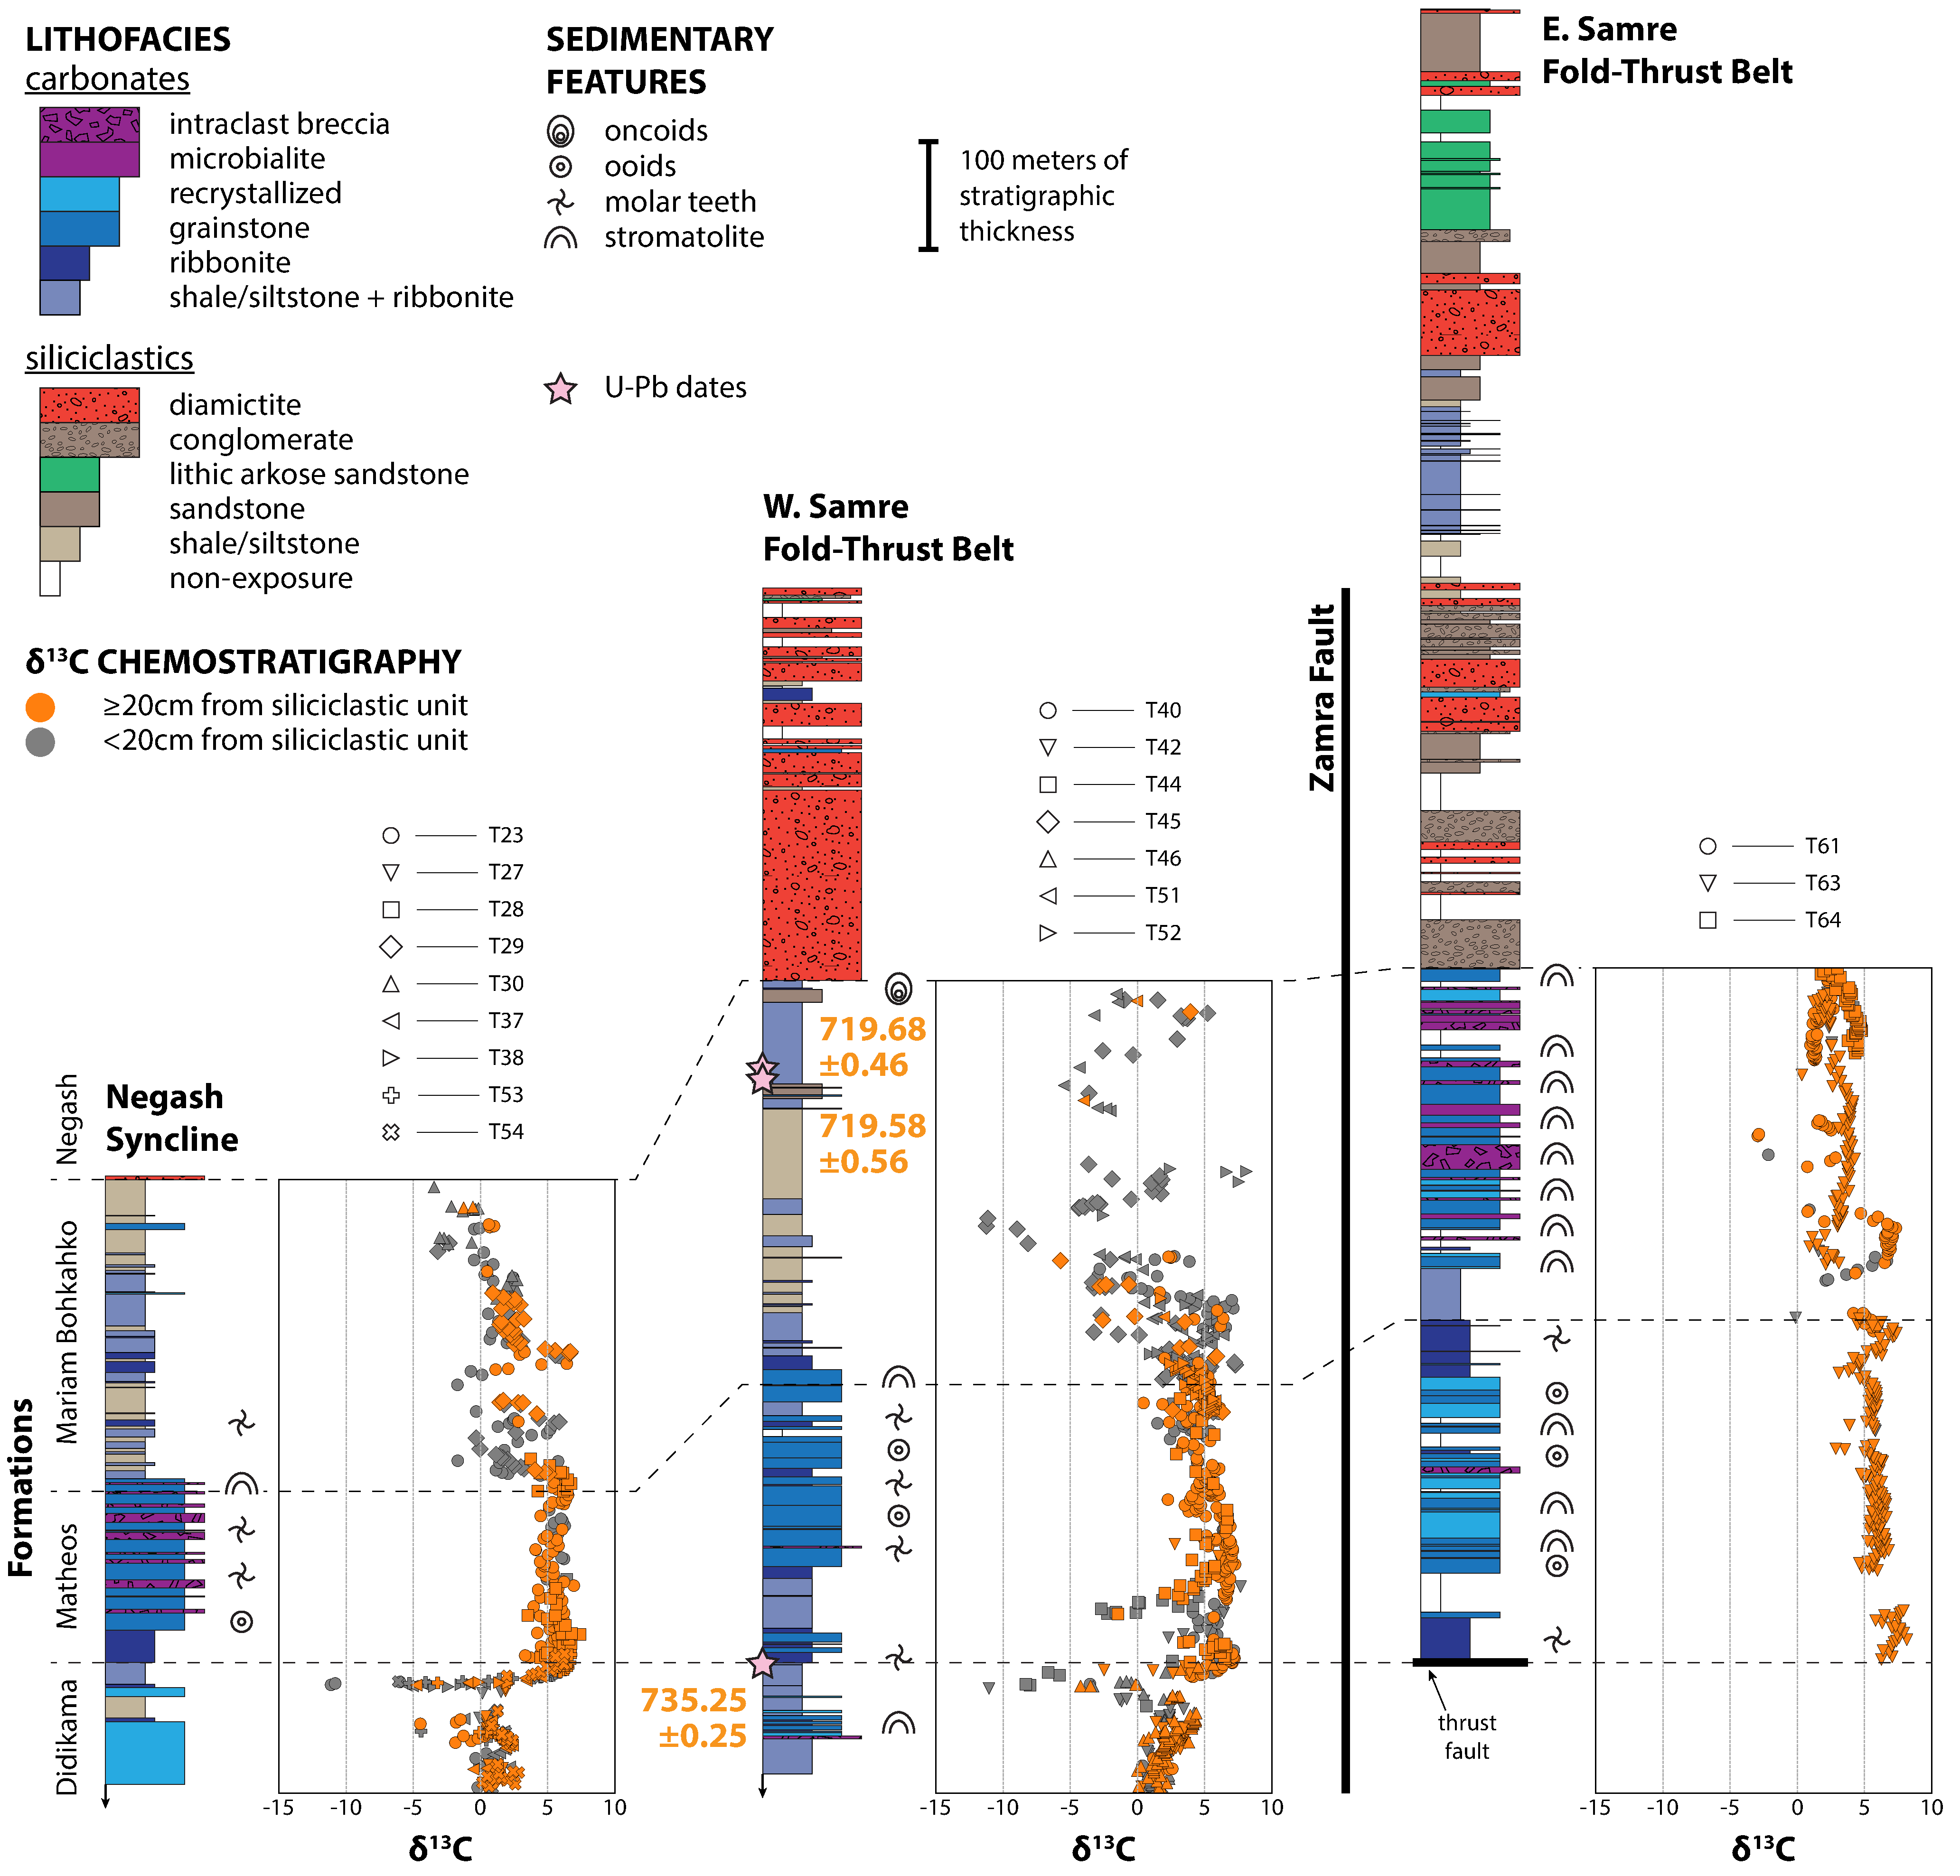
\includegraphics[width=\textwidth]{figures/Tambien/upper-Tambien-comparison.pdf}
	\caption[Lithostratigraphy and \dC chemostratigraphy of the upper Tambien Group.]{Lithostratigraphy and \dC chemostratigraphy of upper Tambien Group exposures in the Negash Syncline and Samre Fold-Thrust Belt (west and east of the Zamra Fault). The stratigraphic sections are representative composites of individually measured sections in each locality with the data within the \dC composite keyed out to each individual section. \dC data are colored based on their stratigraphic distance from the closest siliciclastic unit. U-Pb dates are in units of Ma, and are from \citet{MacLennan2018a}. A more detailed depiction of the contact between the Mariam Bohkahko and Negash formations in the Samre Fold-Thrust Belt is shown in Figure \ref{fig:Sturtian-onset}.}
	\label{fig:upper-Tambien-comparison}
\end{center}
\end{figure}

The Matheos Formation is dominated by limestone and has a thickness $\sim$150-350~m in the Negash Syncline and the Samre Fold-Thrust Belt (Figs. \ref{fig:fence-diagram} and \ref{fig:upper-Tambien-comparison}). In both localities, the blue-grey limestones of the formation form distinctive topographic ridges that are readily identified both in the field and from satellite imagery. In contrast to the Didikama Formation, primary textures are well-preserved.

In the Negash Syncline and west of the major NE-striking thrust fault in the Samre Fold-Thrust Belt (the Zamra Fault; Fig. \ref{fig:Negash-Samre-maps}), the formation begins with grey ribbonite limestone with horizons of molar tooth structures and transitions into grainstone with abundant oolite, intraclast breccia, and molar tooth structures (Fig. \ref{fig:lithofacies}). These lithofacies indicate a shallowing upwards trend with deposition occurring in an energetic shallow-water environment. East of the fault, although the formation begins with the same grey ribbonite limestone with horizons of molar tooth structures that is seen in the other areas, oolite and stromatolitic carbonates are the dominant lithofacies (Fig. \ref{fig:upper-Tambien-comparison}). Deposition of the Matheos Formation to the east of the Zamra Fault also occurred in a shallow-water environment, but one dominated by stromatolites.

\subsubsection{Mariam Bohkahko Formation}

The Mariam Bohkahko Formation is exposed in the Negash Syncline and the Samre Fold-Thrust Belt (Fig. \ref{fig:fence-diagram}). The beginning of the formation is marked by the end of the distinctive blue-grey limestone facies of the Matheos Formation.

In the Negash Syncline and west of the Zamra Fault in the Samre Fold-Thrust Belt, the base of the Mariam Bohkahko Formation consistently is marked by partially dolomitized stromatolitic carbonate (Figs. \ref{fig:lithofacies} and \ref{fig:upper-Tambien-comparison}). These stromatolites are followed by mixed siliciclastic-carbonate sedimentary rocks that are dominated by siltstone. The carbonate beds that are interbedded with the siltstones often are boudined and dolomitized, likely due to their proximity to the core of the large-scale synclines. Some horizons of coarser-grained siliciclastics (up to very fine sandstone) are present toward the top of the formation, some of which are cross-stratified. In some areas, climbing ripples, oolitic grainstones, and oncolites are observed within $\sim$30~m of the top of the Mariam Bohkahko Formation before the contact with the overlying Negash Formation, with carbonate grainstone beds within 1~m of the contact. Overall, these lithofacies suggest deposition in a shallow-water environment.

East of the Zamra Fault, the base of the Mariam Bohkahko Formation consists of siltstones with interbedded ribbonites (Fig. \ref{fig:upper-Tambien-comparison}). The rest of the formation in this area comprises almost entirely of partially dolomitized carbonates, including stromatolites, oncolites, oolitic grainstone, ribbonite, and intraclast breccia, with only rare siliciclastic intervals. Toward the top of the formation, the stratigraphy often comprises \textit{in situ} stromatolites, intraclast breccia with clasts of stromatolites, and minor microbialaminite (Figs. \ref{fig:lithofacies} and \ref{fig:upper-Tambien-comparison}). Again, overall, these lithofacies suggest deposition in a shallow-water environment.

These differences in the stratigraphy of the Mariam Bohkahko Formation across the Zamra Fault indicate different sediment sources and/or depositional environments and potentially significant offset across the fault. To the east, the dominance of carbonate facies (including stromatolites, oncolites, oolites, and microbialaminite) in the Mariam Bohkahko Formation suggest deposition in a shallow-water tropical carbonate belt within the photic zone that lacks significant siliciclastic sediment input. Tidal bypass channels could be transporting silt through this carbonate belt to an outer detrital belt to the west, where minor carbonate beds are interbedded in strata dominated by siltstone. Carbonate interbeds to the west likely represent redeposition of the carbonate sediment being generated in the shallow-water carbonate factory to the east.

Given the importance of the nature of the contact between the Mariam Bohkahko and Negash formations, it is discussed separately in \textit{Onset of the Sturtian Snowball.}

\subsubsection{Negash Formation}

The Negash Formation is exposed in the Negash Syncline and the Samre Fold-Thrust Belt (Fig. \ref{fig:fence-diagram}). In the Negash Syncline and west of the Zamra Fault in the Samre Fold-Thrust Belt, the formation mostly comprises massive diamictite with a silt matrix (Figs. \ref{fig:lithofacies} and \ref{fig:upper-Tambien-comparison}). Clast sizes within the diamictite are variable between pebble and boulder. Clast density also is variable, with clast-poor versus clast-rich horizons. Clasts within the diamictite include carbonate lithologies, some of which retain primary textures allowing them to be identified as ribbonites, grainstone, and ooilitic grainstone. Although not uniquely diagnostic, the facies as well as the carbon isotope composition of these carbonate clasts (see \textit{Diagenetic Considerations}) are consistent with the interpretation that they were derived from the Tambien Group and point to an intra-basinal source. In addition to carbonate clasts, clasts of sandstone, vein quartz, rhyolite, meta-basalt, volcaniclastic breccia, aplite, and granite are present. Detrital zircon geochronology (U-Pb SHRIMP) conducted on matrix combined with clasts of the Negash Formation collected in the Negash Syncline reveal dates dominantly between 850 and 750~Ma with a minor population between 1050 and 950~Ma \citep{Avigad2007a}. Many of these lithologies, as well as the 850 to 750~Ma zircons, could have been sourced from rocks associated with the Arabian-Nubian arcs, some of which had collided and amalgamated by that time \citep{Johnson2014a}. However, the 1050 to 950~Ma zircons, as well as the granitoid clasts, are likely of extra-basinal origin, which is consistent with the interpretation that the diamictite is glacigenic. A minor portion of the Negash Formation in these areas comprises facies that are distinct from the massive diamictite with silt matrix, including: diamictite with a coarse sand matrix, pebble to cobble conglomerates with carbonate and/or metavolcanic clasts, thin beds of limestone ribbonite, fine to coarse lithic arkose sandstones (likely sourced from the proximal arc) with rare pebbles/cobbles, and clast-free sandstone and siltstone (Fig. \ref{fig:upper-Tambien-comparison}).

The Negash Formation frequently is foliated in the core of the Negash Syncline, but also in some outcrops in the Samre Fold-Thrust Belt. This foliation can make it difficult to confidently identify glacigenic sedimentary textures, such as deformation of layers associated with dropstones, and to liberate clasts for the observation of striations. Nevertheless, \citet{MacLennan2018a} and \citet{Miller2003a} identified grooves on cobbles that were interpreted as striations of glacial origin.

East of the Zamra Fault, the Negash Formation is significantly more variable than that west of the fault and in the Negash Syncline, with a smaller proportion of the stratigraphy comprising massive diamictite (Fig. \ref{fig:upper-Tambien-comparison}). The base of the formation in this area can either be massive diamictite, or a clast-supported conglomerate with a dolomitized carbonate matrix and sub-angular carbonate clasts that have facies that are identical to those found in the underlying Mariam Bohkahko (stromatolite and stromatolite breccia) and Matheos (oolite) formations (Fig. \ref{fig:lithofacies}; discussed further in \textit{Onset of the Sturtian Snowball}). In the most representative and continuous Negash Formation section measured in this area, this carbonate breccia is overlain by cm-scale fining upward beds of very fine to fine sandstone. These beds transition into massive diamictite interbedded with medium to coarse sandstones and the carbonate breccia described previously, followed by an interval of siltstones interbedded with cm-scale carbonate ribbonites and occasional horizons of cm-scale coarse poorly sorted sandstones that consist of limestone and lithic fragments. The ribbonites from within this interval are likely the fine-grained products of redeposition of eroded underlying Tambien Group carbonates, given that carbonate precipitation is expected to be thermodynamically inhibited in the cold waters of a global glaciation. Diamictite above and below this interval are almost identical, and the cm-scale carbonate beds are distinct from the thick Sturtian cap carbonate sequences observed in other localities \citep{Kennedy1998a, Hoffman2011a}. To date, no tuffs have been observed in the Negash Formation, preventing the development of direct geochronologic constraints on the formation. The stratigraphically highest observed exposures of the Negash Formation in this eastern Samre Fold-Thrust Belt consist of intervals of massive diamictite with a fine to coarse sand matrix and fine to coarse lithic arkose sandstones with rare pebbles/cobbles.

West of the Zamra Fault, the dominance of massive diamictite may suggest glaciomarine deposition near the grounding line of the local glacier. On the other hand, the relative lack of massive diamictite east of the Zamra Fault could represent proximity to subglacial meltwater channels and/or deposition in an outwash plain slightly more distal from the grounding line of the glacier. Similar to the Mariam Bohkahko Formation, this difference in the stratigraphy of the Negash Formation across the Zamra Fault could be explained by movement along the fault. The Zamra Fault could have initially been a syn-depositional normal growth fault that later got reactivated as a thrust fault during the East African Orogeny, juxtaposing two locales that were once further apart. However, more study of the lithofacies of the Negash Formation is warranted.

\subsection{Basin Development}

Deposition in a back-arc basin is consistent with the geologic context of the Tambien Group. Other sedimentary sequences overlying ca. 850-800~Ma volcanics in western Eritrea and northern Ethiopia have been interpreted as being deposited in back-arc basins on the basis of the trace-element composition of the volcanics and field relationships between the sedimentary sequences and adjacent oceanic-arc rocks \citep{Tadesse1999a, Teklay2003a, Teklay2006a}. Furthermore, mapping within the Arabian-Nubian Shield of Ethiopia, Sudan, and Eritrea has identified several ophiolites within roughly north-south trending suture zones \citep{Berhe1990a}, U-Pb crystallization ages from Arabian-Nubian Shield volcanic and plutonic rocks are dominantly Tonian to Cryogenian in age \citep{Johnson2014a}, Sm-Nd isotopes indicate derivation from juvenile mantle sources, and Nd model ages are dominantly Tonian to Cryogenian \citep{Johnson2014a}. Together, these data support a model wherein the Arabian-Nubian Shield formed through the amalgamation of multiple arcs and associated arc-related basins.

The transition from volcanic and volcaniclastic lithologies of the Tsaliet Group to the mixed carbonate-siliciclastic sediments of the Tambien Group could be associated with slab rollback that caused the arc to migrate away from the initial site of eruption and volcaniclastic deposition, resulting in extensional and flexural accommodation space followed by thermal-isostatic subsidence. The ages of 795.67 $\pm$ 0.82 and 794.29 $\pm$ 0.44~Ma from within and above the lava flows of the Tsaliet Group in the Negash Syncline of the eastern exposures are considerably younger than the eruptive age of 815.29 $\pm$ 0.32~Ma from a tuff within siltstones in the basal Tambien Group in the Tsedia Syncline of the western exposures \citep{Swanson-Hysell2015a}, which indicates that local volcanism continued to generate lava flows in the Negash Syncline while Tambien Group deposition already had begun in the western exposures. This diachronous timing of the transition from volcanism to sedimentation from west to east supports a back-arc basin setting, with the locus of volcanism (recorded by the lava flows in the Tsaliet Group) migrating eastward in present day coordinates. Slab rollback has been well-documented in the the more recent geologic record as a process causing arc migration and accommodating back-arc basin development (e.g. \citealp{Uyeda1979a, Kastens1988a, Schellart2006a}). For example, over the past $\sim$80~Myr, the rollback for the Pacific plate has accommodated the opening of multiple back-arc basins north of New Zealand and has proceeded at rates between $\sim$40-0~km/Myr \citep{Schellart2006a}. Mean rates of trench retreat globally are on the order of 10 km/Myr \citep{Schellart2008a}. Based on the present-day distance in northern Ethiopia that does not account for shortening, the minimum average eastward migration rate of the Tsaliet-Tambien group boundary between the Tsedia Syncline ($\sim$820~Ma) and the Negash Syncline ($\sim$790~Ma) is $\sim$2~km/Myr. This value is well within the range of average slab rollback rates estimated at the Australian-Pacific plate boundary, even if the shortening in the Tsaliet and Tambien groups approaches that estimated for the Himalayan fold-thrust belt (75\%; \citealp{Long2011a}). Furthermore, the broad similarity of the stratigraphy between the Negash Syncline and the Samre Fold-Thrust Belt (a present day lateral distance of $\sim$100~km, which has likely changed little since the time of deposition since the axis of compression during the East African Orogeny was oriented approximately perpendicular to the axis that spans these two locations; \citealp{Stern1994a}) suggests that the Tambien basin was elongate along the present day NNE-SSW direction. This geometry is consistent with structural inversion of a back-arc basin from an extensional to a compressional regime, since the major structural features (synclines, anticlines, and thrust faults) also have NNE-SSW orientations. Tuffs near the base of the Tambien Group also have pumice fiamme in the eastern exposures, and are associated with cobble- to boulder-sized scoria bombs in the western exposures, indicating proximity to an active arc \citep{Swanson-Hysell2015a}. In contrast, tuffs higher in the Tambien Group do not have such associations and are more consistent with having formed through air-fall ash sourced from active arcs further from the basin. Lithofacies of the upper Tsaliet Group and Mai Kenetal and Amota formations also suggest shallower deposition in the eastern exposures relative to the lithofacies of these formations in the west (see \textit{Lithostratigraphy}), which again supports eastward migration of volcanism and associated transgression in this basin. We note, however, that the presence of facies that suggest deposition above wave base throughout the Tambien Group indicates that deposition of the siliciclastic and carbonate sediments overall kept pace with subsidence. The lithologic difference between carbonate-dominated and siliciclastic-dominated portions of the stratigraphy likely is dominantly controlled by time and spatially varying siliciclastic sedimentary input into that particular portion of the basin. The lifespan of Tambien Group deposition (\textgreater100~Myr) also is similar to that of other identified back-arc basins in the geologic record \citep{Woodcock2004a}.

\section{Tambien Group Chemostratigraphy}

Stratigraphic sections across the Tambien Group are correlated to one another by using the geochronologic constraints and aligning both the characteristic lithofacies of the formations and the \dC curve to create a composite Tambien Group \dC and \SrSr chemostratigraphic record (Fig. \ref{fig:fence-diagram}). All geochemical data and the Python code used to assess the degree of alteration of each sample and develop the composite Tambien Group chemostratigraphy are included in the \SI. \dC and \SrSr data developed by \citet{Miller2009a} also are incorporated into our Tambien Group composite. Given that the data from \citet{Miller2009a} were collected from surface transects rather than measured stratigraphic sections, integration into our chemostratigraphic dataset was made based on: A) correlation of sampling localities (shown on maps in \citealp{Miller2009a}) to our geological maps; B) correlation of sample heights and formations (shown approximately in fence diagrams in \citealp{Miller2009a}) to our measured sections; and C) correlation of \dC values.

\subsection{Chemostratigraphic Results}

\begin{figure}[h!]
\begin{center}
	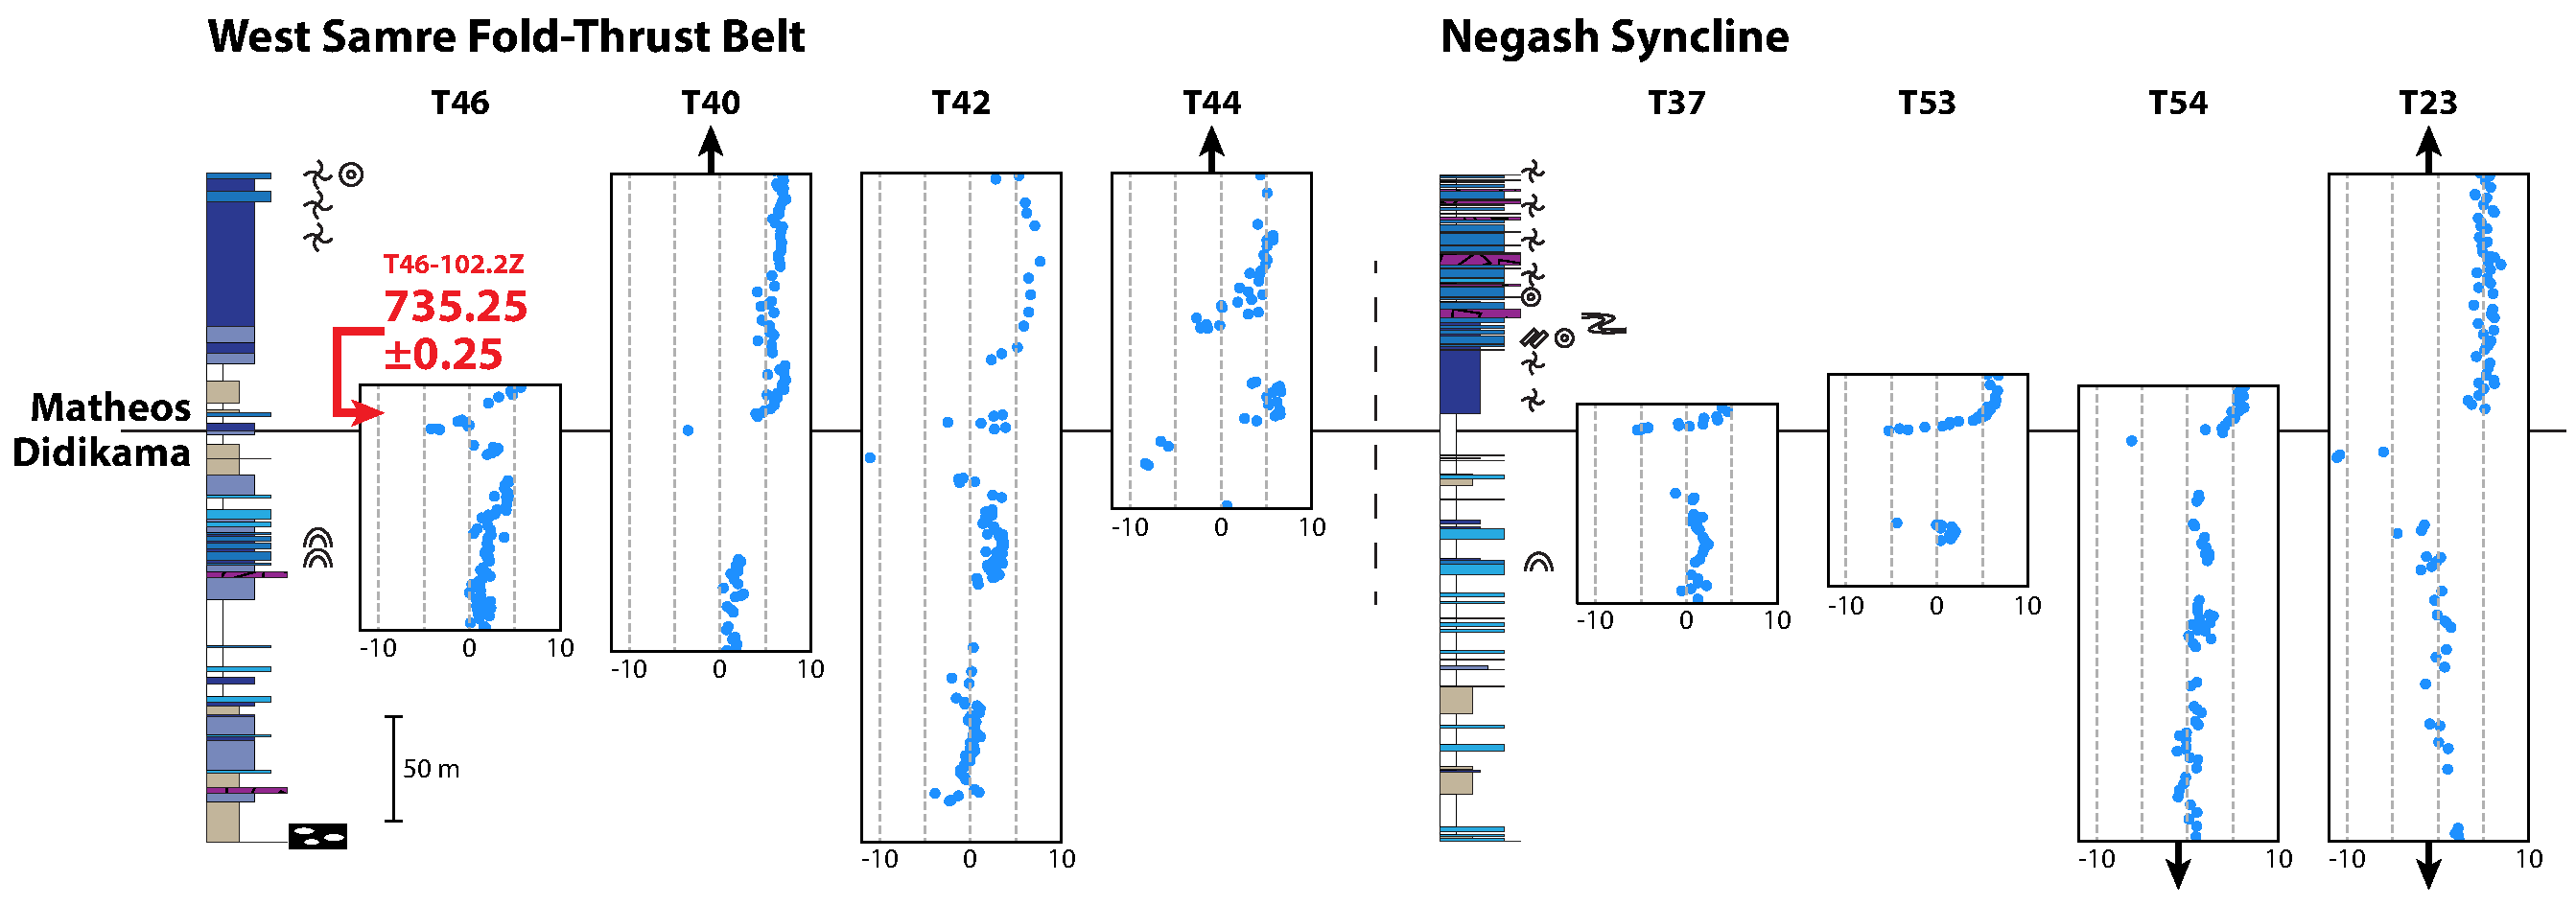
\includegraphics[width=\textwidth]{figures/Tambien/Didikama-Matheos-sections.pdf}
	\caption[Lithostratigraphy and \dC chemostratigraphy from sections that capture the Didikama-Matheos excursion.]{Summary lithostratigraphy and \dC data from sections that capture the Didikama-Matheos excursion from the Samre Fold-Thrust Belt and Negash Syncline. The symbology for the lithofacies and sedimentary structures is the same as that used in Figure \ref{fig:upper-Tambien-comparison}. Black arrows indicate that lithostratigraphic and \dC data continues upwards/downwards for that section, but are not shown.}
	\label{fig:Didikama-Matheos-sections}
\end{center}
\end{figure}

Paired \dC data and U-Pb dates from the lower Tambien Group have led to the interpretation that the negative \dC values within the Assem Formation correlate with the ca. 810-790~Ma Bitter Springs stage \citep{Swanson-Hysell2015a}. However, samples that resolved the onset of the stage (i.e. the descent from $\sim$5\permil to $\sim$-4\permil) had not been identified, due to a lack of carbonate horizons in the lower Tambien Group. New \dC data from carbonates within the lower Werii Formation in the southwestern Tsedia Syncline begin at values of $\sim$5\permil and fall sharply to \textless-5\permil, with values of $\sim$-5\permil for the rest of the Werii Formation, similar to those in the overlying Assem Formation (Fig. \ref{fig:fence-diagram}). We interpret these \dC data to reflect the onset of the Bitter Springs stage, which further supports the hypothesis that the stage has a rapid onset leading into a prolonged global perturbation to the carbon cycle \citep{Maloof2006a, Swanson-Hysell2015a}. After the recovery from the Bitter Springs stage, \dC values are sustained at $\sim$5\permil, before the stratigraphy transitions from the carbonate-dominated Mai Kenetal Formation to the mixed carbonate-siliciclastic Amota and Didikama formations. \dC values from carbonates within these mixed carbonate-siliciclastic parts of the stratigraphy are more scattered than those in carbonate-dominated parts of the stratigraphy. Nevertheless, the majority of the data through the Amota and Didikama formations lie between 0 and 5\permil, and no major excursions are observed. Near the contact between the Didikama and Matheos formations, a large \dC excursion to $\sim$-12\permil is observed, which we will refer to as the Didikama-Matheos excursion (see \textit{Diagenetic Considerations} and \textit{\dC Excursions}; \citealp{Swanson-Hysell2015a, MacLennan2018a}). This \dC excursion now is reproduced in eight sections across the basin (Fig. \ref{fig:Didikama-Matheos-sections}). Following this excursion, \dC values are steady at $\sim$5\permil, before the stratigraphy transitions from the Matheos Formation to the Mariam Bohkahko Formation, which has more variable \dC values. However, we attribute the majority of this scatter within the Mariam Bohkahko Formation to alteration processes that drive \dC to more negative values (see \textit{Diagenetic Considerations} and \textit{\dC Excursions}), and thus we interpret the primary \dC values to be broadly declining from $\sim$5 to $\sim$2\permil in the interval between the Didikama-Matheos excursion and the onset of the Sturtian Glaciation (Fig. \ref{fig:upper-Tambien-comparison}).

\SrSr data that we interpret to be primary (see \textit{Diagenetic Considerations}) have relatively stable values of $\sim$0.7067 in the Mai Kenetal Formation (Fig. \ref{fig:fence-diagram}). These data are followed by a large gap before values of $\sim$0.7063 at the base of the Matheos Formation (Fig. \ref{fig:fence-diagram}). Through the Matheos Formation, \SrSr rises to $\sim$0.7067, before declining to $\sim$0.7063 in the middle of the Mariam Bohkahko Formation. One sample within 25~m of the contact between the Mariam Bohkahko and Negash formations is interpreted to retain primary \SrSr = $\sim$0.70603. However, this sample ([Sr] = 1408~ppm and Mn/Sr = 0.34) barely passes our filtering thresholds used to assess alteration. Although the \SrSr of this sample seems to lie on the projected trajectory of declining \SrSr in the upper Mariam Bohkahko Formation (Fig. \ref{fig:fence-diagram}), more data from the time interval immediately preceding the onset of the Sturtian Glaciation is required to test whether our interpretation of the primary nature of the \SrSr of this sample is robust.

\subsection{Diagenetic Considerations}

\subsubsection{Sample Proximity to Siliciclastic Units}

\begin{figure}[!htbp]
\begin{center}
	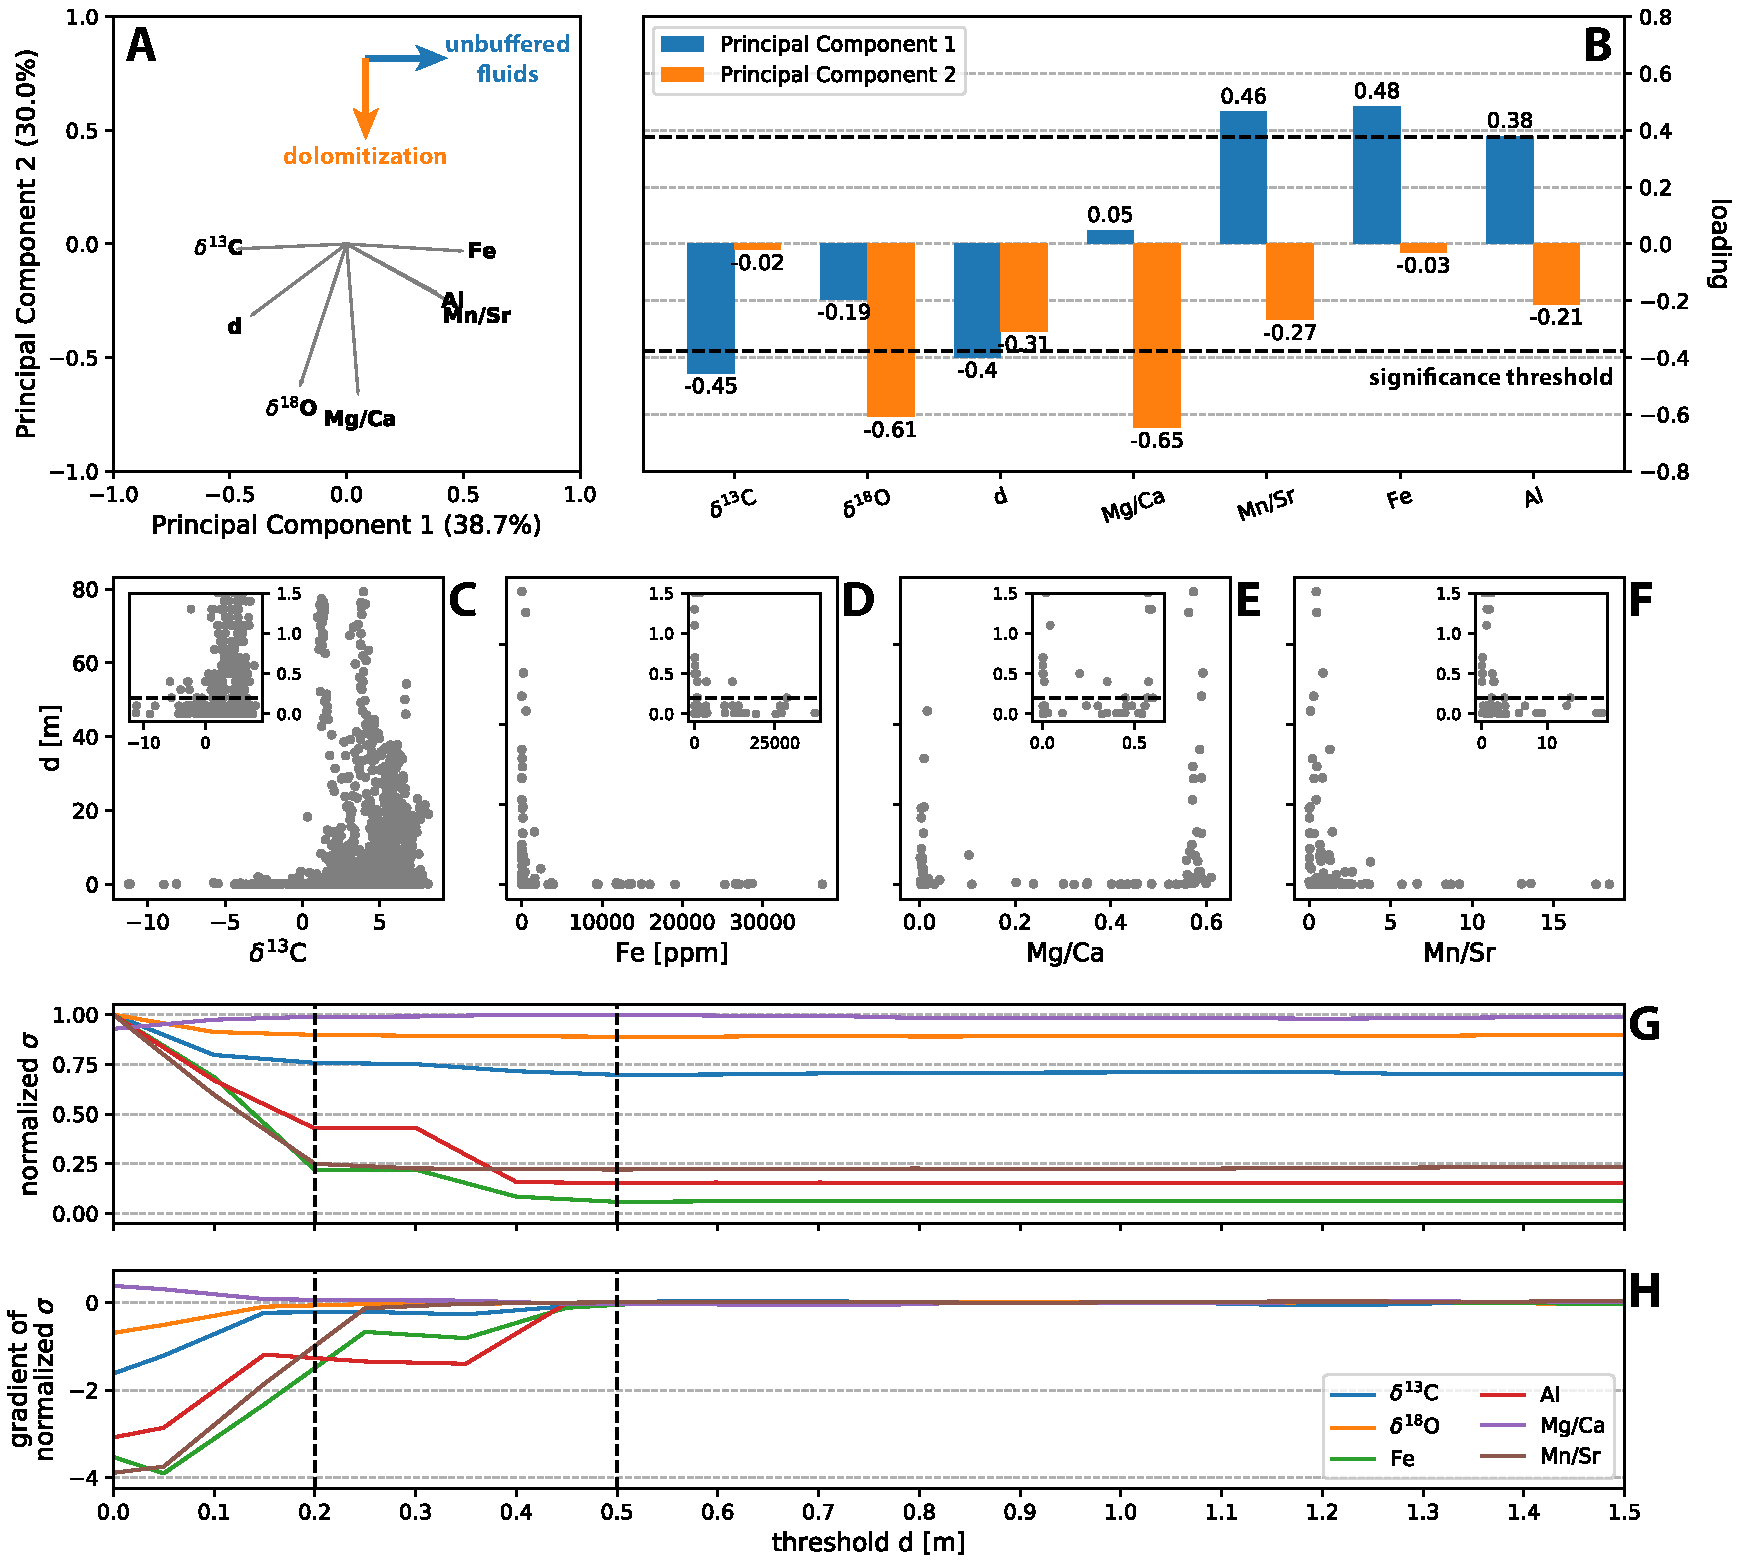
\includegraphics[width=\textwidth]{figures/Tambien/siliciclastic-filtering.pdf}
	\caption[Principal components analysis on carbonate geochemical data.]{\textbf{A)} Loadings plot from a principal components analysis (PCA) on all samples with element concentration data above the Didikama-Matheos excursion. The analysis reveals two main alteration pathways, associated with the first two principal components. \dC and \dsil (the proximity of each carbonate sample to the closest siliciclastic unit) are anti-correlated with the first alteration pathway, which we interpret to be via `unbuffered (with respect to carbonate) fluids.' \textbf{B)} Histogram of loadings/eigenvalues on the first two principal components. The significance threshold is defined as $\sqrt{\frac{1}{\text{number of variables}}}$. \textbf{C-F)} Scatter plots of samples above the Didikama-Matheos excursion. Inset plots have the same x-axes as their parent plots, but have y-axes zoomed in to \dsil 0-1.5~m. The dashed line in the inset plots shows the selected \dsil threshold of 0.2~m. The variance for \dC, Fe, Al, and Mn/Sr increase considerably at low \dsil. \textbf{G)} Standard deviation ($\sigma$) of the remaining data as samples below a given \dsil (x-axis) are removed, normalized to the $\sigma$ when no samples are removed (i.e. all the data). The dashed line at \dsil = 0.2~m denotes where $\sigma$ for \dC falls to background levels, and the dashed line at \dsil = 0.5~m denotes where $\sigma$ for Fe, Al, and Mn/Sr fall to background levels. \textbf{H)} The corresponding gradient of G.}
	\label{fig:siliciclastic-filtering}
\end{center}
\end{figure}

Some of the proposed mechanisms for cooling and the initiation of the Sturtian Snowball Earth have invoked connections between global glaciation and a negative \dC excursion leading into the glaciation. Therefore, constraining the carbon isotopic composition of marine dissolved inorganic carbon during the lead-up to the Sturtian Snowball Earth is particularly important for testing these hypotheses.

There is substantial variability (up to $\sim$10\permil) in the carbon isotopic composition of stratigraphically equivalent Mariam Bohkahko Formation carbonates immediately beneath the Negash Formation (Fig. \ref{fig:upper-Tambien-comparison}). This variability is most pronounced in the Negash Syncline and west of the Zamra Fault in the Samre Fold-Thrust Belt, where the Mariam Bohkahko Formation stratigraphy comprises mixed siliciclastic-carbonate sedimentary rocks that are dominated by siltstone (Fig. \ref{fig:upper-Tambien-comparison}). In contrast, \dC variability is minimal east of the Zamra Fault where the lithofacies of the formation are dominated by carbonate, and \dC values broadly decrease from $\sim$5 to $\sim$2\permil (Fig. \ref{fig:upper-Tambien-comparison}). Given that siliciclastics do not provide a carbonate buffer against altering fluids, it is plausible that carbonate samples collected closer to siliciclastic horizons are less likely to preserve primary \dC and other geochemical signals leading to the higher variability in \dC values observed in the siltstone-rich sections.

To assess whether the proximity of each carbonate sample to the closest siliciclastic unit (\dsil) is a reasonable predictor of \dC alteration, we perform a principal components analysis (PCA) on the samples for which we developed elemental concentration (Al, Fe, Mn, Sr, Mg, Ca) as well as isotope (\dC and \dO) data. A PCA simplifies the complexity in a high-dimensional dataset by geometrically projecting the dataset onto principal components (or eigenvectors), each of which are a linear combination of the original variables in the dataset. The first principal component accounts for as much of the variability in the data as possible, and each following component accounts for as much of the remaining variability as possible. Ultimately, the goal of a PCA is to reduce the dimensionality of the dataset by accounting for the maximum portion of variance present in the dataset using as few principal components as possible. While the lithology of covered intervals without exposure is not known, for determining \dsil we make the conservative assumption that covered units are recessive, fine-grained siliciclastic units. We also exclude samples below and within the Didikama-Matheos excursion, so that we can eliminate the complication of potentially primary fluctuations in the \dC chemostratigraphy increasing the variance in the data. Element concentration data and \dsil are log-transformed to transform these variables into near-normal distributions, then all variables are centered and standardized.

As shown in Figure \ref{fig:siliciclastic-filtering}A and B, we interpret that the PCA reveals two main alteration pathways corresponding to the first two principal components, which together explain 68.7\% of the variance in the dataset (see \SI for a discussion on the selection of these two components). The first pathway (principal component 1) shows high positive loadings on Fe, Al, and Mn/Sr, consistent with alteration via a fluid that has had significant interaction with siliciclastic units prior to interacting with the carbonate samples. The second pathway (principal component 2) shows high negative loadings on Mg/Ca, which is consistent with alteration via dolomitization. Mg/Ca is positively correlated with \dO, which suggests that dolomitization occurred early during the diagenetic history of the carbonates, locking in high \dO values that were later less susceptible to overprinting via warm and/or meteoric low \dO fluids due to the lower reactivity of dolomites relative to limestones. Most importantly, however, the PCA reveals that \dC and \dsil are anti-correlated with the first of these alteration pathways - in other words, high Fe, Al, and Mn/Sr often are associated with low \dC and small stratigraphic distance from a siliciclastic unit (low \dsil) in our carbonate samples. This result suggests that many of the low \dC values in this portion of the stratigraphy where \dC values are scattered are likely a result of alteration via fluids that are unbuffered with respect to carbonate (which we term `unbuffered fluids') that likely have interacted with low \dC organic matter during transit through siliciclastic units. Whether this alteration via unbuffered fluids occurred soon or much after deposition is not constrained by the PCA. At greater distances from the nearest siliciclastic unit (higher \dsil), fluids would have spent more time transiting through carbonates prior to interaction with a sampled horizon, and these carbonate-buffered fluids are not expected to significantly change \dC, Fe, Al, and Mn/Sr.

The results of the PCA are corroborated by the scatter plots shown in Figure \ref{fig:siliciclastic-filtering}C-F -- at the lowest distances from the closest siliciclastic unit (\dsil), the variation in \dC, Fe, Al, and Mn/Sr jumps dramatically. On the other hand, Mg/Ca is bimodally distributed except at low \dsil where intermediate Mg/Ca values are observed. This result suggests that the unbuffered fluids associated with this alteration pathway can cause partial dolomitization, but are not responsible for the vast majority of the dolomitization in the Tambien Group.

To constrain the degree to which these unbuffered fluids have penetrated into the carbonate horizons in the Tambien Group and potentially altered primary \dC, we compute the standard deviation of each of the geochemical variables as samples below a given \dsil are removed (Fig. \ref{fig:siliciclastic-filtering}G and H). The variability in \dC falls to background values at $\sim$0.2~m, and for Fe, Al, and Mn/Sr between $\sim$0.2 and 0.5~m. These results suggest that the characteristic length scale of alteration of Tambien Group carbonates by unbuffered fluids is $\sim$0.5~m, with alteration of \dC being most significant up to $\sim$0.2~m. This difference in overprinting length scales of \dC vs. Fe, Al, and Mn/Sr can be explained by the ability of carbonates to buffer against changes in C more effectively than trace elements.

The results of filtering out samples below various values of \dsil on the \dC composite chemostratigraphy of the Tambien Group are shown in the \SI. As suggested by the analysis of the standard deviations above (Fig. \ref{fig:siliciclastic-filtering}G and H), most large inconsistencies in \dC at any given composite stratigraphic height are removed using the \dsil = 0.2~m threshold, and increasing the threshold beyond that value, in general, simply removes all data in intervals of the composite chemostratigraphy where carbonate horizons are relatively thin.

Notably, data that resolve the Didikama-Matheos excursion as well as the descent into and recovery out of the Bitter Springs stage (but not the prolonged interval of negative values that define the Bitter Springs stage) are partially removed under the \dsil = 0.2~m threshold (Fig. \ref{fig:fence-diagram}), and completely removed by \dsil = 0.5~m (see \SI). Furthermore, the Didikama-Matheos excursion coincides with a major facies transition from siliciclastic-dominated strata to carbonate-dominated strata that defines the Didikama-Matheos formation boundary (Fig. \ref{fig:Didikama-Matheos-sections}). The difference in permeability associated with this facies boundary may have created a significant conduit for fluid flow at this stratigraphic horizon, driving \dC to more negative values than elsewhere in the Tambien Group. Together, these two observations could support an interpretation that the sharp negative \dC excursion at the Didikama-Matheos formation boundary is a product of secondary alteration. It is important to note, however, that several samples within the Didikama-Matheos excursion that record \dC as low as -5\permil, significantly below the \textgreater0\permil values before and after the excursion, are not culled on the basis of the \dsil = 0.2~m threshold. Furthermore, it is important to consider the limitations of this \dC filter based on \dsil. First, the filter is likely not useful at \dsil significantly beyond the characteristic length scale of alteration of Tambien Group carbonates by unbuffered fluids (i.e. $\sim$0.2~m for carbon) - selecting a \dsil threshold significantly above this value would arbitrarily remove \dC data that have not been altered by these fluids. Second, heterogeneity in the distance to which these unbuffered fluids penetrated into Tambien Group carbonates is expected. This method does not account for such spatial heterogeneity, and so samples that fall below the threshold \dsil may or may not have been altered by the unbuffered fluids. Indeed, we find that some samples that we have high confidence are recording primary \dC based on the consistency in \dC values of samples within and between measured sections (e.g. samples with \dC $\sim$5\permil in the Mai Kenetal Formation; Fig. \ref{fig:fence-diagram}) are removed using this approach. On the other hand, we can have relatively high confidence that the \dC values of samples above the threshold \dsil have not been altered by unbuffered fluids. Third, this method takes the conservative approach and assumes that intervals of no outcrop within measured sections are siliciclastic units. Since siliciclastic units (especially fissile siltstones, which dominate the siliciclastic portions of Tambien Group stratigraphy) often are less resilient to weathering than carbonates, the probability that this assumption holds is high within some sections. Nevertheless, the possibility remains that some of these covered intervals are actually carbonates that have been buried by colluvium.

There are several other observations that argue for the primary nature of the Didikama-Matheos excursion. First, high-precision age constraints from zircons in tuffs demonstrate that this \dC excursion occurs at the same time as negative \dC values interpreted as a ca. 735~Ma \dC anomaly observed in other basins around the world (Fig. \ref{fig:composite-chemostratigraphy}, and \textit{\dC Excursions}). Second, the Didikama-Matheos excursion is consistently reproduced across the \textgreater100~km distance between the Samre Fold-Thrust Belt and Negash Syncline (Fig. \ref{fig:Didikama-Matheos-sections}), and wherever samples were collected across the Didikama-Matheos formation boundary, a sharp \dC excursion has been observed. Third, although the driver for the ca. 735~Ma \dC anomaly is not known, it is likely that a perturbation to the carbon cycle of the magnitude required to create such an excursion would be associated with major environmental change and an associated change in lithofacies. Fourth, the samples that record low \dC values in the Didikama-Matheos excursion generally exhibit lower Fe, Al, and Mn/Sr than samples with low \dC above the Didikama-Matheos excursion, suggesting that low \dC Didikama-Matheos excursion samples have been less altered by the unbuffered fluids than low \dC post-Didikama-Matheos excursion samples (see \SI).

Given the balance of evidence for and against the primary nature of the Didikama-Matheos excursion, and given the inherent limitations of the \dC filter based on \dsil, we interpret the excursion to be a primary feature of the record. If these carbonates have been altered by unbuffered fluids, the effect may have been to `deepen' the excursion, rather than creating it from an otherwise stable \dC chemostratigraphy. We find that the primary utility of the filter as described here is to assess which \dC values are primary in intervals of the stratigraphy where time-equivalent carbonates produce inconsistent results (e.g. in the Mariam Bohkahko Formation). Nevertheless, we acknowledge the possibility that the sharp negative \dC excursion at the Didikama-Matheos formation boundary is instead a product of secondary alteration.

\subsubsection{Isotope Conglomerate Test}

\begin{figure}[h!]
\begin{center}
	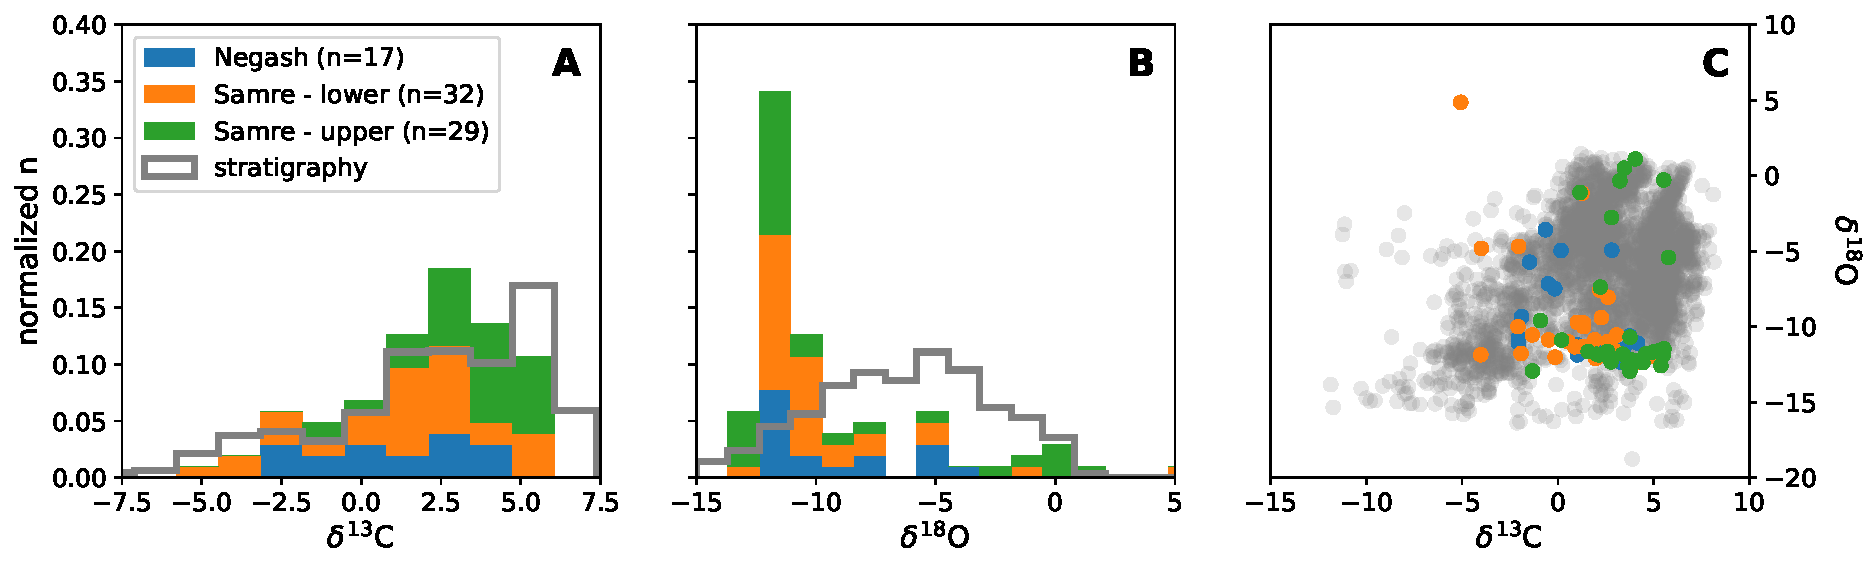
\includegraphics[width=\textwidth]{figures/Tambien/clast-analysis.pdf}
	\caption[Diamictite carbonate clast isotope conglomerate test.]{\textbf{A)} and \textbf{B)} Histograms of \dC and \dO values of carbonate clasts within the diamictite of the Negash Formation from the Negash Syncline and Samre Fold-Thrust Belt. Clasts from the Negash Syncline (n = 17) were sampled from a single horizon. Clasts from the Samre Fold-Thrust Belt (n = 61) were sampled from two horizons (lower and upper) $\sim$100~m stratigraphically apart. \textbf{C)} Cross plot of \dC vs \dO values of the carbonate clasts. In all panels, grey data represent all carbonate samples taken from below the diamictite in the Tambien Group (i.e. from the \textit{in situ} stratigraphy).}
	\label{fig:clast-analysis}
\end{center}
\end{figure}

We perform an isotope conglomerate test on carbonate clasts within the diamictite of the Negash Formation of both the Negash Syncline (n = 17) and the Samre Fold-Thrust Belt (n = 61) (Fig. \ref{fig:clast-analysis}). In such a test, carbonate clasts are sampled to test whether carbon and oxygen isotopes within the clasts were reset to similar \dC and \dO values through either meteoric or burial diagenesis \citep{Husson2012a, Husson2015a}. If the clasts show substantial variability in their isotopic composition, we infer that their isotopic values were acquired prior to deposition in the clastic unit and were not fully reset through burial diagenesis.

The isotope conglomerate test in the Negash Syncline reveals a $\sim$7\permil range in \dC values, and in the Samre Fold-Thrust Belt there is a slightly greater range of $\sim$10\permil. These values are consistent with the carbonate clasts being sourced from the underlying stratigraphy (Fig. \ref{fig:clast-analysis}). However, the \dO values of the clasts in both areas cluster at $\sim$-12\permil, which may indicate that the \dO values of the clasts, unlike the \dC values, largely were reset after the deposition of the Negash Formation. However, the \dC and \dO of the clasts do not appear to be correlated, which supports the interpretation that the clasts preserve near primary \dC even for clasts where the \dO was altered. This indication of preferential preservation of primary \dC over \dO is consistent with carbon being more rock-buffered against altering fluids than oxygen \citep{Banner1990a}.

\subsubsection{Sr Isotopes}

\begin{figure}[h!]
\begin{center}
	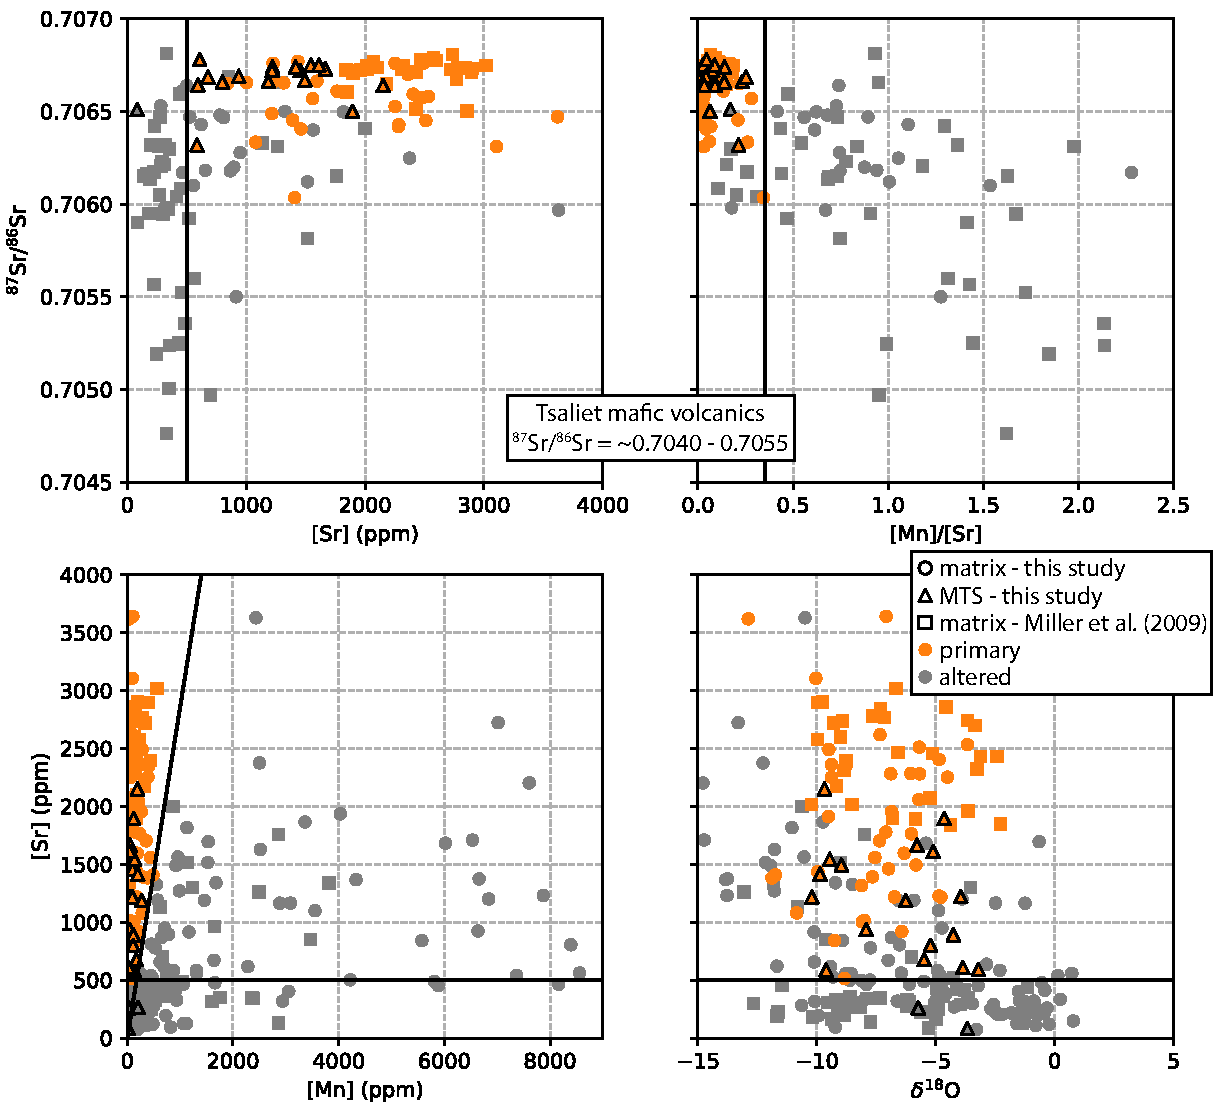
\includegraphics[width=0.8\textwidth]{figures/Tambien/Sr-diagenesis.pdf}
	\caption[Cross plots of Sr and Mn in carbonates.]{Cross plots of [Sr] and Mn/Sr against \SrSr, and [Mn] and \dO against [Sr] for data presented in this study and \citet{Miller2009a}. Black lines illustrate the thresholds used to interpret primary versus altered \SrSr ([Sr]\textgreater500~ppm and Mn/Sr\textless0.35). MTS = molar tooth structure.}
	\label{fig:Sr-diagenesis}
\end{center}
\end{figure}

Relative to C isotopes, Sr isotopes in carbonates are more vulnerable to secondary alteration (e.g. \citealp{Banner1990a}). Trace element geochemistry can be used to assess the degree of such alteration. Mn/Sr values are a commonly-used indicator of alteration, since interaction with secondary fluids tend to increase [Mn] and decrease [Sr] \citep{Brand1980a, Banner1990a, Jacobsen1999a}. Furthermore, low [Sr] makes \SrSr more susceptible to overprinting since less exchange is required to alter the original strontium isotopic ratio \citep{Brand1980a, Veizer1989a, Banner1990a}. As in other studies (e.g. \citealp{Halverson2007b}), we apply a filter based on minimum [Sr] and maximum Mn/Sr in order to exclude \SrSr values from samples that are more likely to be altered. To select appropriate [Sr] and Mn/Sr thresholds for our samples, we take advantage of the presence of molar tooth structures in the Tambien Group, since these structures consist of high purity calcite that precipitated from seawater within the host carbonate mud prior to dewatering and lithification. As a result, these structures are more likely to record primary geochemical signals relative to the surrounding micrite due to a lack of Rb-containing clay and more limited recystallization (Fig. \ref{fig:MTS-petrography}). Given that all molar tooth structure samples cluster at Mn/Sr\textless0.35, and all molar tooth structure samples except one have [Sr]\textgreater500~ppm, these values are used as filtering thresholds to generate a record that is more likely to be reflective of primary \SrSr (Fig. \ref{fig:Sr-diagenesis}). We find that the \dC and \SrSr values from molar tooth structures are similar to that of immediately adjacent micrite that pass the elemental thresholds (see \SI). This similarity suggests that micritic samples from the Tambien Group (provided that they pass the elemental thresholds set above) also are capable of preserving primary geochemical signals, and supports their use alongside calcite from molar tooth structures in reconstructing Tonian marine \SrSr.

Fluid-rock geochemical models generally predict that overprinting results in a sharp increase in \SrSr below a threshold [Sr] \citep{Banner1990a, Jacobsen1999a}. These models assume that the altering fluid has high \SrSr resulting from interaction with radiogenic rocks with high \SrSr prior to interacting with the carbonates. However, as discussed by \citet{Miller2009a}, the altering fluids that are responsible for overprinting in the Tambien Group would have had significant interaction with juvenile arc volcanics and volcaniclastics with low \SrSr before interacting with the carbonates, since the Tambien Group was deposited atop of the arc volcanics and volcaniclastics of the Tsaliet Group. Two samples of mafic volcanics of the Tsaliet Group in the proximity of the Tsedia Syncline have \SrSr values of 0.704047 and 0.705406, which confirms these expected low values. As a result, we do not expect to see a sharp increase in \SrSr below the threshold [Sr]. Instead, we expect to see a decrease in \SrSr at low [Sr] due to the altering fluid containing Sr sourced from juvenile arc material. This latter relationship is observed in the data (Fig. \ref{fig:Sr-diagenesis}). We note that the majority of the low [Sr] and high Mn/Sr samples that have low (and excluded) \SrSr  values come from \citet{Miller2009a}; many of the data developed in this study are from samples that were screened for [Sr] and Mn/Sr prior to \SrSr analysis.

\section{Tonian-Cryogenian Chemostratigraphic Composite}

\begin{figure}[h!]
\begin{center}
	\includegraphics[width=\textwidth]{figures/Tambien/composite-chemostratigraphy.pdf}
	\caption[Tonian-Cryogenian \dC and \SrSr chemostratigraphic composite.]{Tonian-Cryogenian \dC and \SrSr chemostratigraphic composite. The paleogeographic reconstructions are included to illustrate the approximate geometry of Rodinia (assembled vs. dispersed) through the Tonian.}
	\label{fig:composite-chemostratigraphy}
\end{center}
\end{figure}

Combined with U-Pb ID-TIMS dates on zircons from \citet{Swanson-Hysell2015a} (815.29 $\pm$ 0.32, 788.72 $\pm$ 0.24, and 787.38 $\pm$ 0.14~Ma), \citet{MacLennan2018a} (735.25 $\pm$ 0.25, 719.58 $\pm$ 0.56, and 719.68 $\pm$ 0.46~Ma), and this study (Table \ref{tab:geochronology}), \dC and \SrSr data from the Tambien Group (\citealp{Miller2009a, Swanson-Hysell2015a}; this study) now comprise the most temporally well-constrained pre-Sturtian chemostratigraphic dataset to date. These data are combined with other chemostratigraphic and geochronologic datasets from Neoproterozoic sedimentary rocks in other localities around the world to generate an updated composite Tonian chemostratigraphy (Fig. \ref{fig:composite-chemostratigraphy}). We use the Tambien Group \dC curve as the backbone for making correlations with other datasets. Tonian \dC and \SrSr data within the composite come from the Akademikerbreen Group of Svalbard \citep{Halverson2007b,Halverson2007a}, the Eleanore Bay Supergroup of East Greenland \citep{Cox2016a}, the Bitter Springs Group of Australia \citep{Swanson-Hysell2010a, Cox2016a}, the Fifteenmile Group of Canada \citep{Macdonald2010a, Cox2016a}, the Little Dal Group of Canada \citep{Halverson2006a, Halverson2007b}, the Coates Lake Group of Canada \citep{Halverson2006a, Halverson2007b, Rooney2014a}, the Shaler Supergroup of Canada \citep{Asmerom1991a, Jones2010a}, the Dalradian Supergroup of Scotland \citep{Sawaki2010a}, Proterozoic carbonates of the Uchur–Maya and Turukhansk regions of Siberia \citep{Bartley2001a, Cox2016a}, and the Karatau Group of the Urals \citep{Kuznetsov2006a, Cox2016a}. Cryogenian \dC and \SrSr data within the composite come from the Tsagaan-Olam Group of Mongolia \citep{Brasier1996a, Bold2016a}, the Hay Creek Group of Canada \citep{Rooney2014a}, the Adelaide Rift Complex of South Australia \citep{Swanson-Hysell2010a, Rose2012a}, and the Otavi Group of Namibia \citep{Halverson2005a, Halverson2007b}.

Correlations between datasets are made using absolute age constraints where possible - otherwise, the characteristic negative \dC anomalies of the ca. 800~Ma Bitter Springs stage and the ca. 735~Ma anomaly that is referred to in the literature as the Islay anomaly (although this name is potentially problematic; \citealp{Fairchild2018a}) are used to align datasets. The same criteria for assessing altered \SrSr values that were used in the original publications are applied here, unless our analysis of \SrSr vs. [Sr] and \SrSr vs. Mn/Sr suggested a different criteria for alteration. However, even when different criteria are applied for a particular dataset, the resulting \SrSr curve is similar to that presented in the original study with little difference for the large-scale \SrSr trends through the Tonian. The details of the methodology, details regarding the compiled data, and a link to the Python code used to develop the Tonian-Cryogenian chemostratigraphic composite are included in the \SI.

\section{Discussion}

\subsection{Onset of the Sturtian Snowball}

\subsubsection{Geochronology}

Energy balance models of Snowball Earth initiation propose that, once ice sheets reach $\sim$30$^{\circ}$ latitude, the ice-albedo positive feedback overwhelms negative feedbacks on temperature, causing Earth's surface temperature to plummet and ice to advance to the equator on the time scale of less than a few thousand years \citep{Baum2001a, Hoffman2002a, Pollard2005a}. In other words, energy balance models predict that, at the resolution of U-Pb ID-TIMS dating, all low-latitude areas were covered by ice at the same time. While this hypothesis is supported by climate models of varying complexity, a direct field test for the synchronous onset of any of the Snowball Earth episodes has not been made. In order to perform such a test, high-precision ages from as close as possible to the onset of glacigenic deposits in as many different basins as possible is required. However, despite the fact that glacigenic deposits associated with the Sturtian Snowball Earth have been identified in numerous basins around the world \citep{Hoffman2009a}, very few of these basins have direct geochronologic data that precisely constrains the onset of the glacigenic deposits in their respective basins.

Prior to data from the Tambien Group, the best age constraints on the start of the Sturtian Glaciation came from northwestern Canada where U-Pb ID-TIMS on zircons from a volcanic tuff within glacial diamictite and from a rhyolite underlying this diamictite yielded weighted mean ages of 716.9 $\pm$ 0.4 and 717.43 $\pm$ 0.14~Ma respectively \citep{Macdonald2010a, Macdonald2018a}. Given that thick volcanic units have the potential to obscure sedimentary evidence of glaciation, the 717.43 $\pm$ 0.14~Ma age from the rhyolite cannot be interpreted to be pre-glacial in this basin without ambiguity. Age constraints for the onset of Sturtian glacigenic deposits also come from other basins around the world, but provide looser constraints than the dates from northwestern Canada. U-Pb ID-TIMS on detrital zircons from a volcaniclastic unit underlying Sturtian diamictite in Arctic Alaska yielded a maximum depositional age of 719.47 $\pm$ 0.29~Ma \citep{Cox2015a}. These data cannot rule out that the onset of continental ice in Arctic Alaska significantly post-dated 719.47 $\pm$ 0.29~Ma, especially since an unconformity separates the volcaniclastic unit from the diamictite. U-Pb ID-TIMS on zircons from a tuffaceous graywacke within a Sturtian diamictite in Oman yielded an age of 711.52 $\pm$ 0.31~Ma \citep{Brasier2000a, Bowring2007a}. This minimum age constraint on the onset of continental ice in Oman is consistent with the data from northwestern Canada, but is too young to reliably test the rapid onset of low-latitude glaciation. U-Pb secondary-ion mass spectrometry (SIMS) dates on zircons from tuffaceous slates underlying Sturtian diamictite in South China yielded ages of 715.9 $\pm$ 2.8 and 716.1 $\pm$ 3.4~Ma, also consistent with dates from northwestern Canada. However, zircons from these tuffaceous slates range in age from 705 to 827~Ma \citep{Lan2014a} with large uncertainty on individual dates, and the \textit{in situ} methods used on these samples do not chemically abrade the zircon prior to analysis, which combined with lower precision makes it difficult to identify Pb-loss compared to dates developed using ID-TIMS.

An estimated age of the base of the glacial deposits in the Tambien Group is between 718.0 and 716.4~Ma at the 95\% confidence level \citep{MacLennan2018a}. This constraint is too imprecise to conclude that low-latitude glaciation was as globally synchronous as energy balance models predict. Nevertheless, this result is consistent with synchronous onset of deposition of the Negash Formation and the glacigenic deposits in northwestern Canada.

\subsubsection{Lithostratigraphy}

\begin{figure}[!htbp]
\begin{center}
	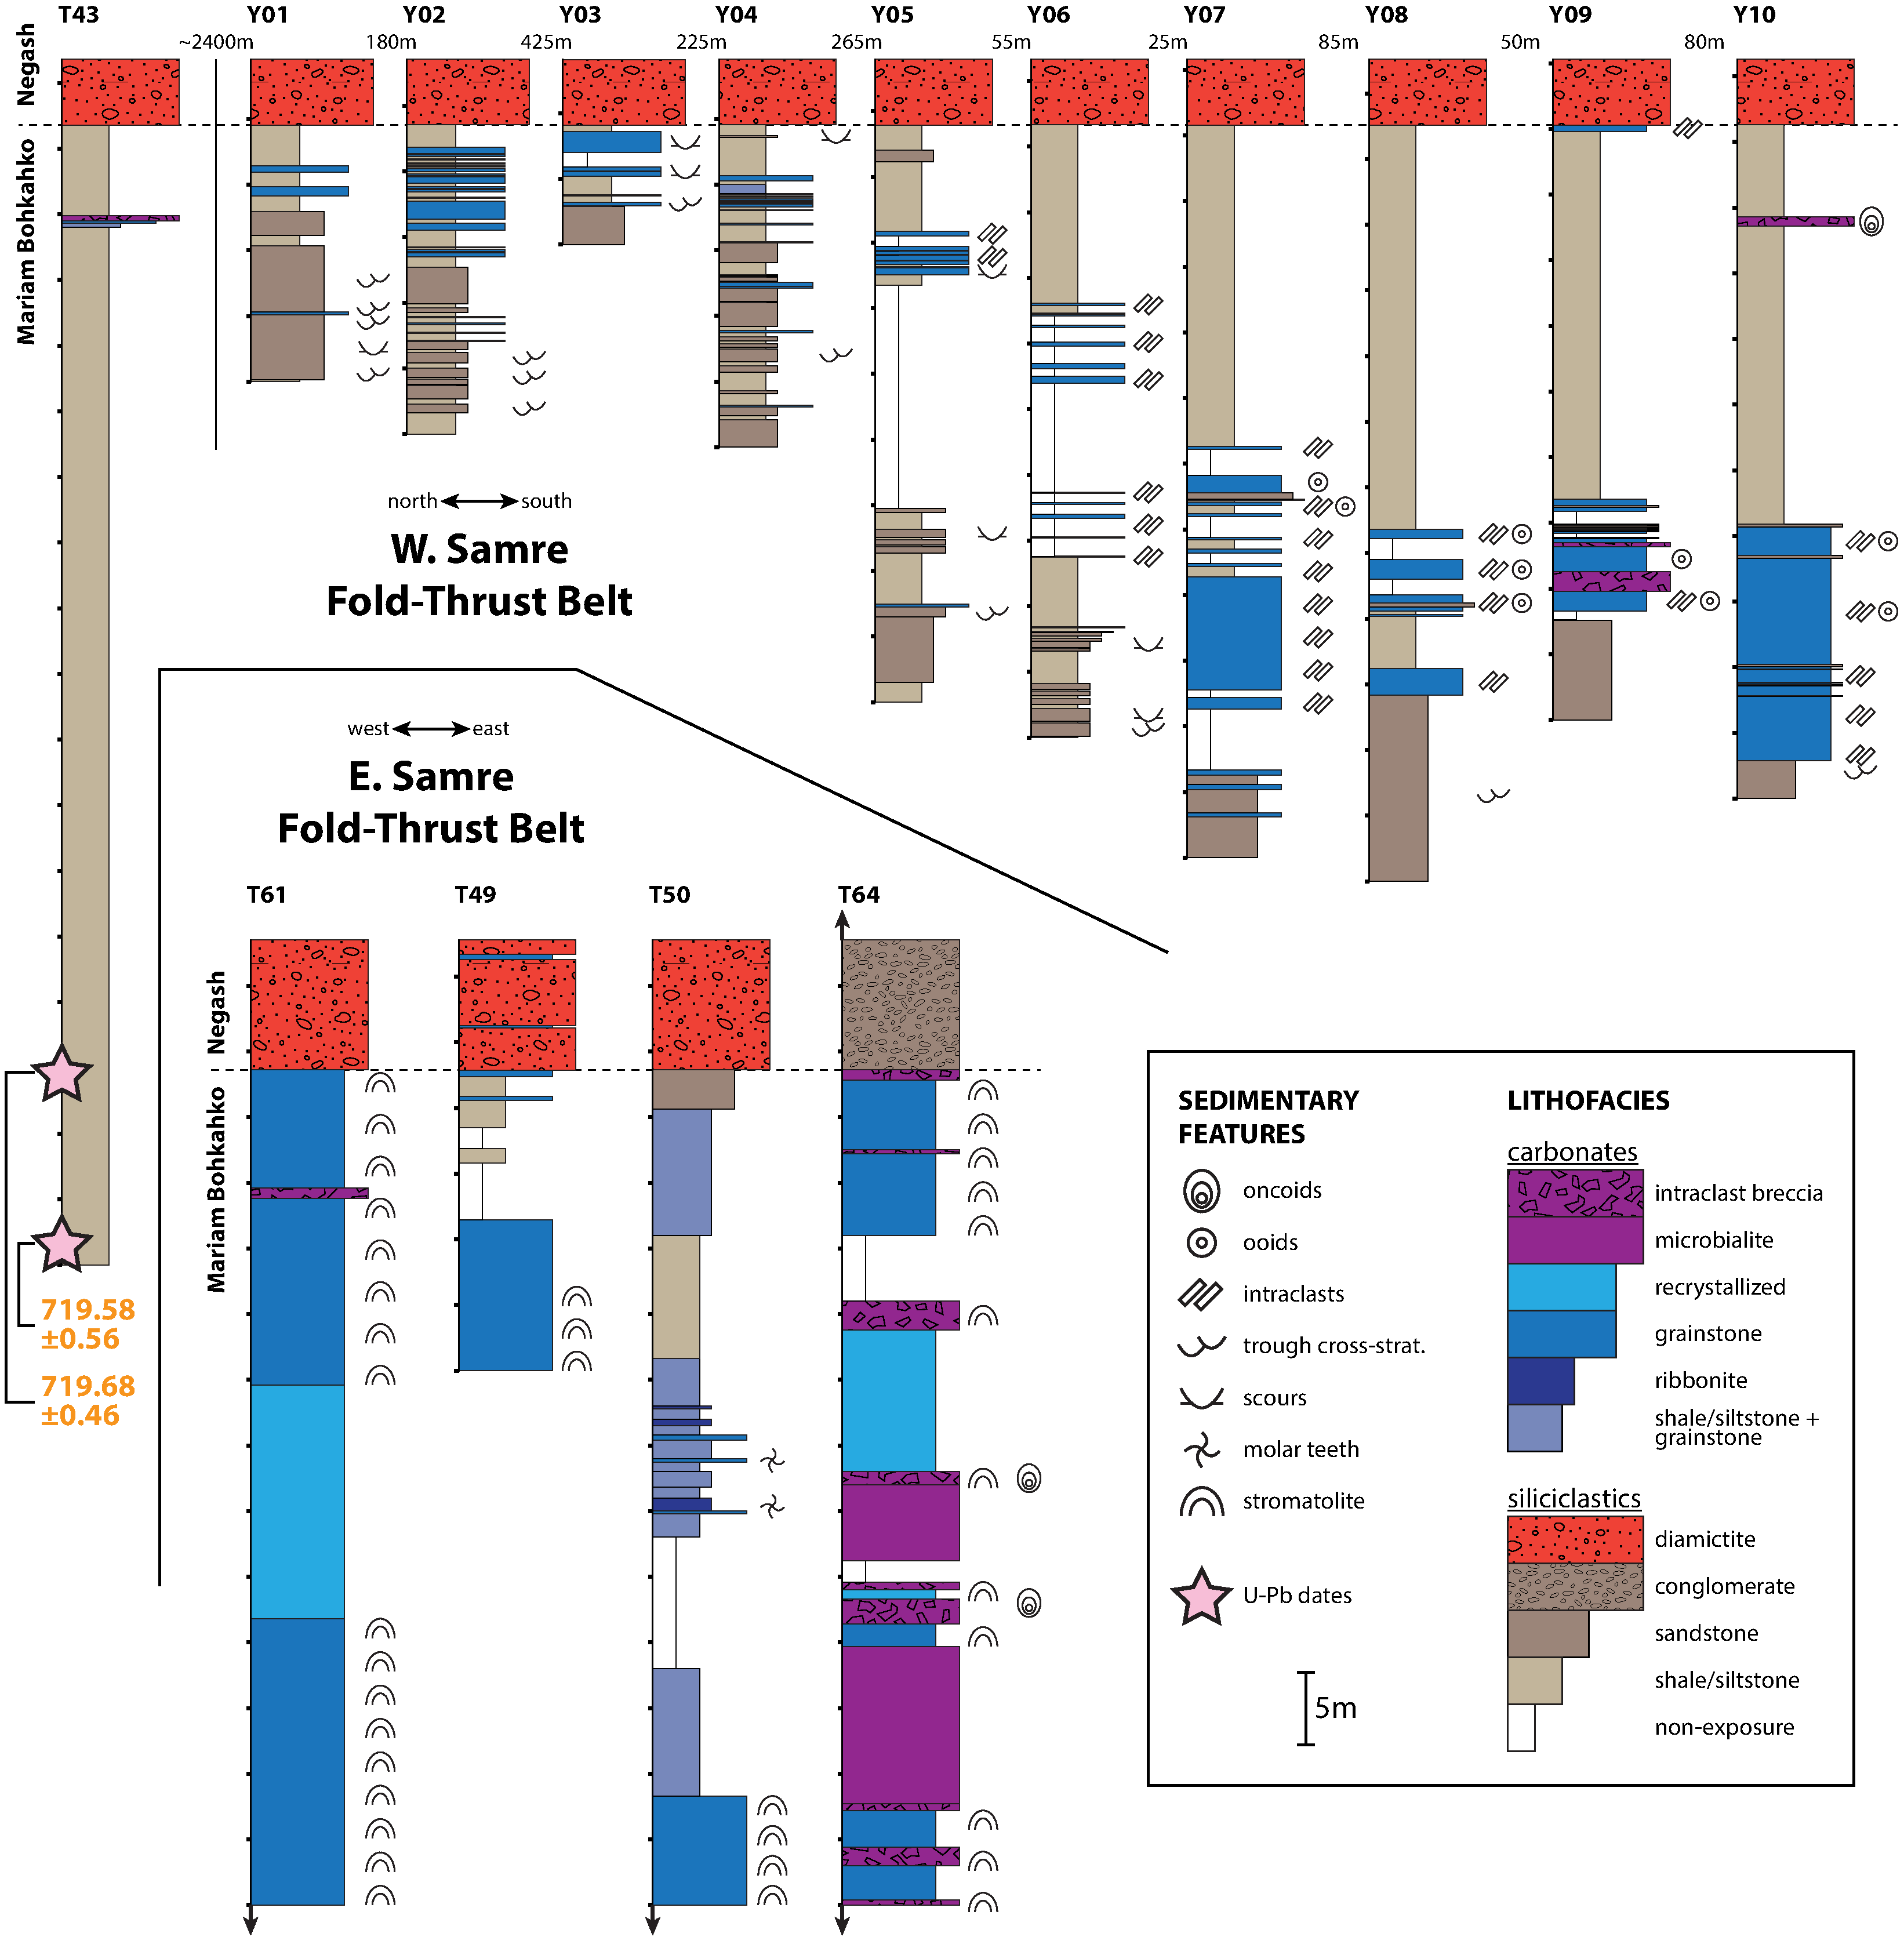
\includegraphics[width=\textwidth]{figures/Tambien/Sturtian-onset.pdf}
	\caption[Lithostratigraphy near the contact between the Mariam Bohkahko and Negash formations.]{Lithostratigraphy near the contact between the Mariam Bohkahko and Negash formations in the Samre Fold-Thrust Belt. In the western Samre Fold-Thrust Belt, sections shown here were measured from north to south along the eastern limb of the major syncline west of the Zamra Fault, except for T43 which was measured along the western limb (Fig. \ref{fig:Negash-Samre-maps}). These sections are representative of the nature of this contact in that area. Meter values above the stratigraphic columns indicate the distance along bedding strike between each of the measured sections. In the eastern Samre Fold-Thrust Belt, sections shown here were measured in three different synclines east of the Zamra Fault near the Zamra River (Fig. \ref{fig:Negash-Samre-maps}), and are organized from west to east. Black arrows indicate that lithostratigraphic data continues upwards/downwards for that section, but are not shown. Tick marks to the left of each stratigraphic column represent 5~m intervals.}
	\label{fig:Sturtian-onset}
\end{center}
\end{figure}

In addition to the geochronologic constraints consistent with synchronous onset of low-latitude glaciation, the evolution of the depositional environment as recorded by the sedimentary lithofacies leading into the Sturtian Glaciation can add insight into the nature of glacial onset. West of the Zamra Fault in the Samre Fold-Thrust Belt (Fig. \ref{fig:Negash-Samre-maps}), the upper $\sim$50~m of the Mariam Bohkahko Formation consists of siltstones and very fine sandstones interbedded with minor carbonates (Figs. \ref{fig:upper-Tambien-comparison} and \ref{fig:Sturtian-onset}). These carbonates are mostly grainstone beds that are generally \textless50~cm thick, and in many places are within a few meters of or in direct contact with the basal diamictite of the Negash Formation. Trough cross-stratification and scour surfaces are common sedimentary features in these strata, as well as carbonate rip-up clasts and ooid grains within the grainstones. In two measured sections, a 60-70~cm oncolite horizon (Fig. \ref{fig:lithofacies}) is observed 7.0 and 23.2~m below the basal diamictite respectively. Together, these lithofacies suggest deposition in or near a shallow-water environment with significant siliciclastic sediment input, proximal to a warm shallow-water carbonate factory that occasionally delivered carbonate sediment to this part of the basin during storms. Notably, we do not observe any change in this depositional environment leading up to the basal diamictite, nor do we observe any outcrop-scale erosional unconformities between the Mariam Bohkahko and Negash formations. Instead, this contact is characterized by the sudden appearance of pebble-sized clasts within previously clast-free siltstones, making it look like a conformable contact. Although accumulation rates are expected to vary significantly between lithofacies, especially on short time scales, \citet{MacLennan2018a} estimated an average long-term accumulation rate of the Matheos and Mariam Bohkahko formations between 2.8-3.5~cm/kyr at the 95\% confidence level. Given that the exact contact (within a few centimeters) between the Mariam Bohkahko and Negash formations is often poorly exposed, if we assume that this accumulation rate estimate holds to first-order for the uppermost Mariam Bohkahko Formation, the fact that we do not observe any change in the warm tropical shallow-water depositional environment leading up to the basal diamictite is consistent with energy balance models that predict that ice advanced to the equator on the time scale of less than a few thousand years \citep{Baum2001a, Hoffman2002a, Pollard2005a}. While the contact appears planar at the outcrop scale, it is possible that there is an erosional unconformity between the two formations. Such an unconformity, for instance via glacial scouring, could be called upon to explain the northward thinning of the uppermost siltstone unit in Figure \ref{fig:Sturtian-onset}, as well as the northward thinning of the Mariam Bohkahko Formation as a whole near the southern nose of the syncline just west of the Zamra Fault (Fig. \ref{fig:Negash-Samre-maps}). Lateral variability in the sequence of lithofacies between measured sections in the uppermost Mariam Bohkahko Formation west of the Zamra Fault could instead reflect lateral variability in basin topography and/or flow patterns during storm events, and the northward thinning of the Mariam Bohkahko Formation as a whole could be explained by structural thickening via isoclinal folds close to the nose of the syncline just west of the Zamra Fault and/or structural thinning via increased boudinaging of carbonate beds moving northward away from the nose of this syncline (see \textit{Lithostratigraphy}). In any case, zircons in volcanic tuffs within the Mariam Bohkahko Formation 73.6 and 85.3~m below the base of the Negash Formation in this area yield U-Pb ID-TIMS ages of 719.68 $\pm$ 0.46 and 719.58 $\pm$ 0.56~Ma respectively (Fig. \ref{fig:Sturtian-onset}; \citealp{MacLennan2018a}). Given that the geochronologic constraints from northwestern Canada suggest that global glaciation was ongoing by 716.9 $\pm$ 0.4~Ma \citep{Macdonald2018a}, that energy balance models predict that ice advanced to the equator on the time scale of less than a few thousand years \citep{Baum2001a, Hoffman2002a, Pollard2005a}, and that tens of meters of sediments continued to be deposited between the eruption of these two tuffs and the first occurrence of diamictite in the Tambien Group, the ages from the Mariam Bohkahko Formation indicate minimal (if any) erosion of the Mariam Bohkahko Formation west of the Zamra Fault.

East of the Zamra Fault in the Samre Fold-Thrust Belt (Fig. \ref{fig:Negash-Samre-maps}), the nature of the contact between the Mariam Bohkahko and Negash formations is more variable than to the west (Figs. \ref{fig:upper-Tambien-comparison} and \ref{fig:Sturtian-onset}). Stromatolites are ubiquitous in the carbonates of the Mariam Bohkahko Formation in this area, and in some cases lie directly in contact with the basal diamictite of the Negash Formation. However, in other cases, siltstones and very fine sandstones interbedded with minor grainstones and ribbonites lie between these stromatolites and the basal diamictite. These siliciclastics with carbonate interbeds could represent a change in water depth or a transition to siliciclastic sediment input into this part of the basin. In the eastern-most syncline of the Samre Fold-Thrust Belt (Fig. \ref{fig:Negash-Samre-maps}), the uppermost Mariam Bohkahko Formation consists of stromatolites, microbialites, and intraclast breccias with stromatolite and oncoid clasts (Fig. \ref{fig:lithofacies}), suggesting deposition in a very shallow warm tropical environment that was conducive to the formation of microbial mats. The base of the Negash Formation in this syncline consists of a distinctive \textgreater45~m thick clast-supported conglomerate composed of sub-angular carbonate clasts within a dolomitized carbonate matrix (Fig. \ref{fig:Sturtian-onset}), instead of the massive diamictite with a silt matrix observed in all other areas. The origin of this carbonate conglomerate is enigmatic, but it could represent a subglacial fan at the mouth of a subglacial channel, a terminal moraine, an olistolith (e.g. \citealp{LeHeron2014a}), or a subglacial channel conglomerate. It is therefore plausible that the contact between the Mariam Bohkahko and Negash formations is unconformable in this eastern-most syncline, especially since no geochronologic data for strata in this area have been developed. However, we do not observe any indication of an erosional unconformity between the Mariam Bohkahko and Negash formations further to the west, and therefore the juxtaposition of marine carbonates, especially stromatolites, with the basal diamictite lends further support to the hypothesis of rapid cooling immediately prior to the glaciation and sudden advance of ice toward the equator.

\subsection{\dC Excursions}

The mechanism(s) behind the exceptionally large negative \dC excursions in the Neoproterozoic remain(s) a mystery. Proposed mechanisms for the excursions include: a decrease in the ratio of organic to inorganic carbon burial resulting from colder conditions suppressing organic productivity \citep{Kaufman1997a, Hoffman1998a}, oxidation of a large dissolved organic carbon pool \citep{Rothman2003a}, enhanced export of organic matter from the upper ocean into anoxic deep water where dissolved and particulate organic carbon is remineralized \citep{Tziperman2011a}, precipitation of authigenic carbonate during early diagenesis \citep{Schrag2013a}, interactions of hydrocarbon-influenced fluids with carbonates during diagenesis \citep{Derry2010a}, and meteoric diagenesis in response to sea level fall \citep{Swart2012a}. Some of these proposed mechanisms for large negative \dC excursions imply that the excursions are global in nature, and therefore synchronous between basins, while others imply local processes that would not necessarily lead to the excursions being recorded in the same age rocks between basins (but see \citealp{Swart2008a}). Furthermore, some of these proposed mechanisms draw connections between large negative \dC excursions and the onset of glaciation.

Data from the Tambien Group add new constraints to this debate. A volcanic tuff (sample T46-102.2Z) adjacent to carbonates with \dC = $\sim$0\permil was identified $\sim$4~m above the $\sim$-12\permil nadir of the large negative excursion near the Didikama-Matheos formation boundary (Fig. \ref{fig:Didikama-Matheos-sections}). Zircons from this tuff yield a weighted mean age of 735.25 $\pm$ 0.88~Ma (including all external uncertainties; \citealp{MacLennan2018a}) using U-Pb ID-TIMS. This age is consistent with geochronologic constraints from within a similar large negative \dC excursion in the Windermere Supergroup of northwestern Canada (referred to as the Islay anomaly in the literature): \citet{Rooney2014a} obtained a Re-Os age of 732.2 $\pm$ 3.9~Ma (including all external uncertainties) from black shales adjacent to carbonates with \dC = $\sim$0\permil and $\sim$200~m above the nadir of the excursion, and \citet{Strauss2014a} obtained a Re-Os age of 739.9 $\pm$ 6.1~Ma (including all external uncertainties) from black shales adjacent to carbonates with \dC = $\sim$-4\permil and $\sim$5~m below the nadir of the excursion. These three dates suggest that the Didikama-Matheos excursion records the same perturbation to the carbon cycle as that in the Windermere Supergroup. Furthermore, although no direct reliable age constraints have been developed, sharp negative \dC excursions interpreted to be correlative to this ca. 735~Ma anomaly in the Windermere Supergroup also have been observed in the Dalradian Supergroup of Scotland \citep{Sawaki2010a}, the Akademikerbreen Group of northeastern Svalbard \citep{Halverson2007a, Hoffman2012a}, and the Windermere Supergroup (Coates Lake Group) of northwestern Canada \citep{Halverson2006a}. Together, these data suggest that a large negative \dC excursion occurs synchronously at ca. 735~Ma in at least two separate basins and potentially globally, and that it precedes the Sturtian Glaciation by $\sim$18~Myr \citep{MacLennan2018a}. We refer to this excursion, which we interpret to be global, as the `735~Ma anomaly.'

Most Tonian stratigraphic sequences either do not host carbonates in the interval immediately preceding the onset of the Sturtian Glaciation, or have missing time associated with an unconformity. Carbonate stratigraphy from northwestern Canada \citep{Halverson2006a, Macdonald2010a, Rooney2014a} and northeastern Svalbard \citep{Halverson2007a} are interpreted to end at or soon after the 735~Ma anomaly (Fig. \ref{fig:composite-chemostratigraphy}). The Coppercap Formation of the Coates Lake Group of northwestern Canada preserves carbonate stratigraphy that records \dC values \textgreater5\permil after the nadir of the 735~Ma anomaly \citep{Halverson2006a, Rooney2014a}, but if the duration of the 735~Ma anomaly (from the initiation of the downturn in \dC values through to the full recovery) is $\sim$1~Myr \citep{MacLennan2018a} and sediment accumulation rates in the Coates Lake Group are constant, the top of this succession would have an age \textgreater730~Ma. However, the Dalradian Supergroup of Scotland may preserve carbonates significantly younger than 735~Ma. \dC values in carbonates of the Garbh Eilach Formation of the Dalradian Supergroup are sustained at $\sim$-5\permil for $\sim$50~m of stratigraphy before gradually increasing to values of $\sim$1\permil over $\sim$10~m of stratigraphy \citep{Fairchild2018a}. These negative \dC values are referred to as the Garvellach anomaly. The weakly positive values are then sustained through the $\sim$10~m of stratigraphy that are interpreted by \citet{Fairchild2018a} to represent a conformable transition into the Sturtian glacial deposits of the Port Askaig Formation. However this interpretation is not without ambiguity, since no direct geochronologic constraints exist for the Garbh Eilach Formation, and the \SrSr data from the carbonates within this formation \citep{Fairchild2018a} are too scattered to use for nuanced chronostratigraphic intepretation. Therefore, it is possible that the intermittent subaerial exposure suggested by the sedimentary features in the upper Garbh Eilach Formation (such as gypsum pseudomorphs; \citealp{Fairchild2018a}) obscures a significant unconformity, and that the Garvellach anomaly may be correlative to the 735~Ma anomaly. Furthermore, the intermittent subaerial exposure could have exposed Garbh Eilach Formation carbonates to meteoric alteration, or created a depositional environment with limited connection to the open ocean. If so, the low \dC values of the Garvellach anomaly could be a result of local processes that do not reflect global marine \dC at the time of deposition.

On the other hand, our analysis of the geochemical data indicates that \dC values are sustained at $\sim$5\permil following the recovery from the 735~Ma anomaly in the Tambien Group, then remain at positive values with a broad decrease to values of $\sim$2\permil through the Mariam Bohkahko Formation up to the contact with the Negash Formation, with low \dC values in the Mariam Bohkahko Formation being a result of secondary alteration via unbuffered fluids (see \textit{Diagenetic Considerations}; Fig. \ref{fig:upper-Tambien-comparison}). Furthermore, geochronologic constraints demonstrate that carbonate stratigraphy from the Tambien Group continues well past the 735~Ma anomaly until at least ca. 719.6~Ma - at most only a few million years before the onset of Sturtian Glaciation (Fig. \ref{fig:upper-Tambien-comparison}). This makes the Tambien Group host to the most demonstrably complete pre-Sturtian (from ca. 820~Ma until 0 to 2~Myr before the onset of global glaciation) carbonate stratigraphy studied to date, and suggests that no large negative \dC excursion was associated with the onset of the Sturtian Glaciation. However, if further work demonstrates that the Garbh Eilach Formation is conformable with Sturtian glacial deposits and that the low \dC values in that formation reflect global marine \dC at the time of deposition, then the Garvellach anomaly must be between $\sim$719-717~Ma and not recorded in the Tambien Group, and could be associated with the onset of the Sturtian Glaciation.

Other sharp high-amplitude Neoproterozoic \dC excursions have been interpreted to be global signals that are temporally disconnected from low-latitude glaciation, such as the Cryogenian inter-glacial Taishir excursion (Fig. \ref{fig:composite-chemostratigraphy}; \citealp{Bold2016a}) and the Ediacaran Shuram-Wonoka excursion \citep{Husson2015a}. Together, these conclusions suggest that proposed mechanisms to explain at least some of these sharp high-amplitude \dC excursions: 1) do not have to be consistent with low \textit{p}CO$_{2}$ and the onset of low-latitude glaciation; and 2) should have the capacity to explain synchronicity in at least a number of basins around the world.

\subsection{Pre-Sturtian \SrSr and the Drivers of Planetary Cooling}

\subsubsection{Large Igneous Provinces}

\begin{figure}[h!]
\begin{center}
	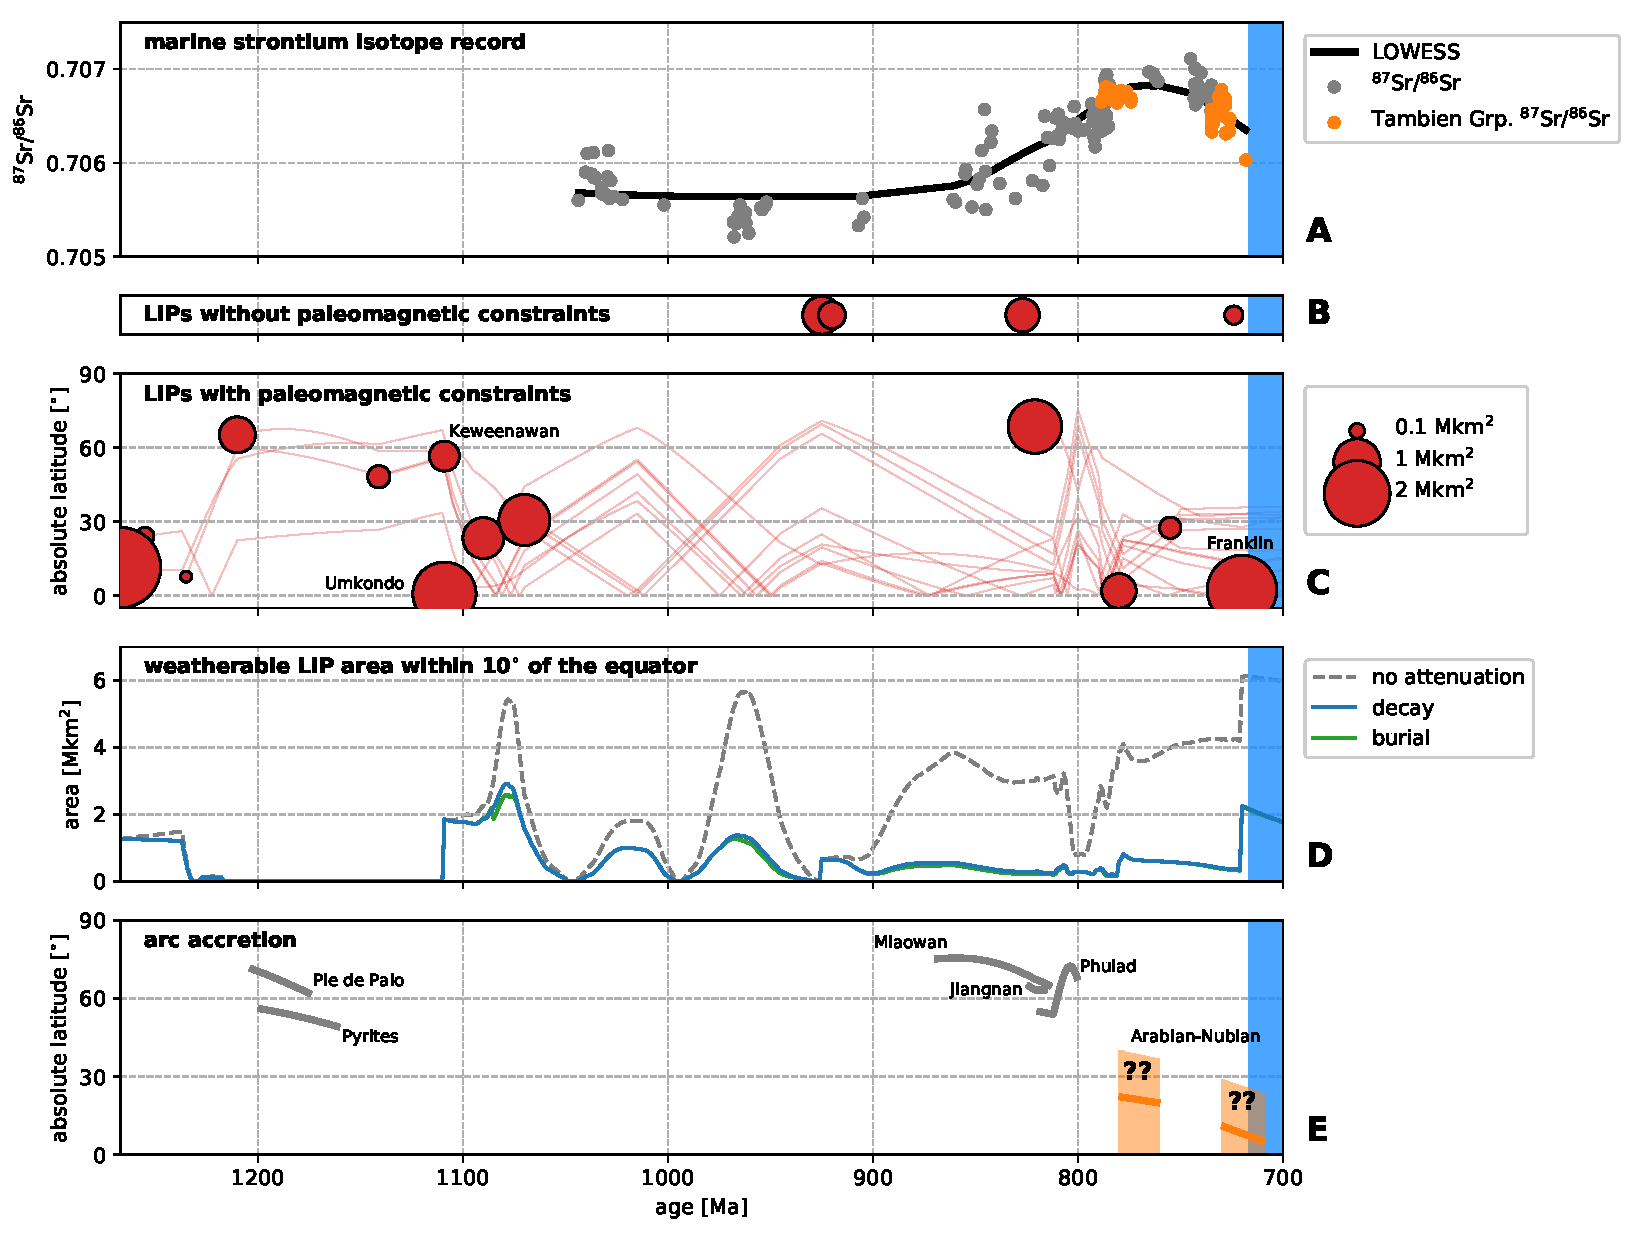
\includegraphics[width=\textwidth]{figures/Tambien/SrSr-LIPs.pdf}
	\caption[Tonian \SrSr and large igneous provinces.]{\textbf{A)} Composite \SrSr. The black line is a locally weighted scatterplot smoothing (LOWESS) line - using 45\% of the data when estimating each y-value resulted in a line that neither over- nor under-represented major trends in the \SrSr data. \textbf{B)} Emplacement timing and area of LIPs (adapted from \citealp{Ernst2017a}) without paleomagnetic constraints. \textbf{C)} Emplacement timing, area, and latitude of LIPs (adapted from \citealp{Ernst2017a}) with paleomagnetic constraints. The lines represent the tracks of the centroids of each LIP after emplacement, obtained from a paleogeographic model \citep{Swanson-Hysell2019a} which incorporates a pair of true polar wander events ca. 810 and 790~Ma \citep{Maloof2010a, Swanson-Hysell2012a}. \textbf{D)} Weatherable LIP area within 10$^{\circ}$ of the equator. The three lines represent three different treatments of LIPs after emplacement (see \textit{Pre-Sturtian \SrSr and the Drivers of Planetary Cooling}). \textbf{E)} Centroids of arc accretion events. The paleolatitude of the Arabian-Nubian accretion events are poorly constrained. The shaded orange region represents the approximate range of latitudes that Arabian-Nubian arc accretion could have occurred at, based on the paleolatitude of India and the African cratons. The orange line represents a single model position for Arabian-Nubian arc accretion that is consistent with existing constraints. In all panels, the blue bar represents the Sturtian Glaciation.}
	\label{fig:SrSr-LIPs}
\end{center}
\end{figure}

One of the most prominent proposed mechanisms for the initiation of the Sturtian Snowball Earth argues that the emplacement of large igneous provinces (LIPs) at low latitudes contributed to the onset of the snowball climate state by enhancing planetary weatherability, leading to a lower atmospheric CO$_{2}$ concentration (the `Fire and Ice' hypothesis; \citealp{Godderis2003a, Cox2016a}). Central to this hypothesis is the fact that mafic lithologies have high weathering rates as well as high concentrations of Ca and Mg that are liberated through chemical weathering and ultimately sequester carbon through carbonate precipitation \citep{Dessert2001a}. Furthermore, there is an apparent increase in the area and frequency of continental flood basalts from ca. 860~Ma onward \citep{Cox2016a}, culminating in the eruption of the 2.225$\times$10$^{6}$~km$^{2}$ Franklin LIP (Fig. \ref{fig:SrSr-LIPs}; \citealp{Ernst2008a}) around the time of Sturtian Glaciation initiation. At this time, paleogeographic reconstructions (e.g. \citealp{Li2008a}) place the Franklin LIP at low latitudes where chemical weathering rates are expected to be highest due to relatively high temperatures and runoff rates. We assess these arguments below through the lens of the newly temporally-calibrated composite \SrSr curve.

The strontium isotopic composition of the oceans is sensitive to the relative weathering flux from different lithologies, and thus provides a record that could give insight into the `Fire and Ice' hypothesis. Sr enters the ocean from a number of distinct sources: weathering of continental lithologies, hydrothermal interaction with mid-ocean ridges, and weathering of island arcs and oceanic island basalts \citep{Richter1992a}. Continental lithologies can be divided into the broad categories of carbonates, juvenile igneous rocks (such as basalt), and older cratonic rocks (such as gneiss and granite). Importantly, each of these lithologies have different weatherabilities, Sr concentrations, and Sr isotopic compositions \citep{Allegre2010a}. In particular, juvenile volcanic lithologies have relatively low \SrSr and are readily weathered, whereas older cratonic lithologies have relatively high \SrSr and are less readily weathered \citep{Dessert2003a}. The higher \SrSr in cratonic lithologies arises as a result of higher concentrations of Rb in differentiated crust where $^{87}$Rb decays to $^{87}$Sr. $^{87}$Sr also is able to accumulate for a long time in ancient cratonic rocks. Sr leaves the ocean primarily through the formation of carbonate minerals (aragonite/calcite/dolomite), which record the \SrSr of ocean water at the time of formation \citep{Brand2004a}. The Sr isotopic composition of the ocean is effectively homogenous at any given time, since the residence time of strontium in the oceans ($\sim$3-5~Myr) is much longer than the mixing time of the ocean ($\sim$1000~yr) \citep{Broecker1982a}. Thus, the \SrSr of the oceans, and therefore unaltered marine carbonates, commonly is interpreted as a proxy for the relative globally averaged fluxes coming from each of the four sources (subaerial weathering of continental carbonates, subaerial weathering of continental radiogenic lithologies, subaerial weathering of continental and oceanic juvenile lithologies, and hydrothermal interaction with mid-ocean ridges) at any given point in time. Therefore, if there was a large increase in the weathering of juvenile material associated with low-latitude LIP emplacement immediately prior to the Sturtian Snowball Earth as the `Fire and Ice' hypothesis argues, the \SrSr of the oceans is expected to respond by significantly decreasing.

The global composite Tonian \SrSr curve is flat at low values of $\sim$0.7055 until ca. 860~Ma when there is an increase up to \SrSr values of $\sim$0.7070 by ca. 770~Ma (Figs. \ref{fig:composite-chemostratigraphy} and \ref{fig:SrSr-LIPs}). There is a subsequent decrease back down to values of $\sim$0.7060 leading up to the initiation of the Sturtian Glaciation ca. 717~Ma. This decrease in \SrSr interrupts the otherwise increasing \SrSr values from ca. 880~Ma onwards that culminates in values $\sim$0.7090 by 600~Ma \citep{Halverson2007a}. There may be additional shorter time scale trends in the global composite Tonian \SrSr curve, but given the scatter in the data at any given time interval, the uncertainty in the precise correlation of the curves between some basins, and the susceptibility of the strontium isotopic composition of carbonates to diagenetic alteration, we choose to focus on interpreting the broader and more robust trends described above.

In Figure \ref{fig:SrSr-LIPs}, the \SrSr curve is plotted along with the emplacement timing, area, and latitude of LIPs in order to evaluate proposed connections between the two. Estimates of original emplacement extents are adapted from \citet{Ernst2017a}, which were drawn to include the full surface extent of all presently-exposed dikes, sills, and volcanics interpreted to be associated with each LIP. For some LIPs, this approach may over-estimate the original surface extent, given that subsurface intrusions could extend over a broader area than the surface volcanics. The polygons also assume complete surface coverage between wide-spread remnants, which could also lead to an over-estimate of the original surface extent. On the other hand, the original extent outlines could also under-estimate the surface area for some LIPs where flows have been eroded and feeder dikes are not exposed or poorly documented. The movements of LIPs after emplacement are determined using a paleogeographic model that incorporates available paleomagnetic constraints. In addition to paleolatitude, the post-emplacement tectonic and erosional history of each LIP is important for considering the effect that a LIP will have on planetary weatherability. For example, without active uplift, soil shielding from regolith development on low-relief LIPs could significantly decrease the local weatherability of a LIP \citep{Gabet2009a, Hartmann2014a, Godderis2017b}. Furthermore, the thickness of this regolith is dependent on the local climate \citep{Norton2014a}. Ultimately, all LIPs will cease weathering at some point, either through burial or complete erosion. As in \citet{Park2019a}, we construct simplified post-emplacement models for LIPS and plot how these scenarios impact the total weatherable area of LIPs within the tropics in Figure \ref{fig:SrSr-LIPs}D. We define the tropics to be within 10$^{\circ}$ of the equator based on the modern zonal-average distributions of temperature and precipitation, which appear to have been stable through time \citep{Evans2006a}. In the `no attenuation' model, weatherable LIP areas are held constant from the time of emplacement (i.e. no post-emplacement processes are accounted for). This model is intended as an end-member reference as LIPs do not persist indefinitely for the reasons described above. In the `decay' model, the weatherable area of each LIP undergoes exponential decay from the time of emplacement, with a half-life of 100~Myr. This model follows the approach of \citet{Godderis2017a} and the implemented 100~Myr half-life is within the range of observed values for younger, better-constrained LIPs. The `burial' model is identical to the `decay' model, except that we account for burial of the ca. 1109~Ma Keweenawan LIP at ca. 1085~Ma by removing it from the model at that time, given that this region thermally subsided and the volcanics were buried by sediment \citep{White1997a, Ojakangas2001a, Swanson-Hysell2019a}. We note that accounting for the burial of the Keweenawan LIP in the `burial' model does not significantly affect the area of weatherable LIPs in the tropics in our post-emplacement models since the LIP has a relatively small area confined to a continental rift. It is important to note that, while broadly representative, these three models are an oversimplification of the true post-emplacement histories for several reasons. For instance, all LIPs (with the exception of the Keweenawan LIP) are treated identically, when instead they may have experienced very different tectonic histories that could result in very different weathering histories. Furthermore, global and local climate would have been sensitive to the paleogeography and paleotopography at any given time step, which together may have created different temperature and runoff conditions at each LIP. For example, the topography of the Himalaya-Tibetan plateau is linked to the Asian monsoons, which introduces significantly higher precipitation in affected areas compared to the zonal average for that latitude \citep{Zhisheng2001a}. Nevertheless, the `decay' and `burial' models are likely much closer to the true post-emplacement histories and associated LIP area in the tropics than the `no attenuation' model.

Between ca. 1270 and 1110~Ma, LIP emplacement is relatively frequent (Fig. \ref{fig:SrSr-LIPs}C). However, these LIPs are either emplaced at mid- to high latitudes, or drift there soon after emplacement, resulting in a minimal area within the tropics (Fig. \ref{fig:SrSr-LIPs}D). At ca. 1110~Ma, the Umkondo LIP (Kalahari craton) is emplaced at low latitudes, followed closely by the Keweenawan (Laurentia craton), SW Laurentia, and Warakurna (Australia craton) LIPs at mid-latitudes, leading to a significant increase in LIP area within the tropics (Fig. \ref{fig:SrSr-LIPs}D). After the emplacement of these four LIPs, there are no identified LIP emplacement events over the next $\sim$150~Myr until ca. 920~Ma, but several Mesoproterozoic LIPs drift through the tropics during this time. As described above, it is unclear whether each of these LIPs were still exposed well enough to increase global weatherability when they drifted through the tropics, but, if the post-emplacement models (Fig. \ref{fig:SrSr-LIPs}D) reasonably approximate the effect of the true post-emplacement histories, then relatively large areas of weatherable LIPs pass through the tropics between ca. 1100 and 920~Ma. The weathering of these LIPs in the tropics could lead to a relatively high contribution to the global weathering flux coming from juvenile rocks passing through the warm and wet tropics and provide an explanation for the low \SrSr values observed throughout this period (Fig. \ref{fig:SrSr-LIPs}A). The Dashigou (North China craton) and Gangil-Mayumbia (Congo craton) LIPs are next emplaced ca. 920~Ma (Fig. \ref{fig:SrSr-LIPs}B). However, no direct paleomagnetic constraints exist for these two LIPs, and their paleolatitudes at the time of emplacement are uncertain. In the paleogeographic model, the Gangil-Mayumbia LIP is at low latitudes at the time of emplacement, but this position is poorly constrained. Nevertheless, given its relatively small area, its contribution to global weatherability is likely to be small, even if emplaced within the tropics. Between ca. 880 and 780~Ma, Mesoproterozoic LIPs continue to transit through the tropics. However, our post-emplacement models predict that the weatherable area of these \textgreater$\sim$200~Myr old LIPs has decayed to small values by this time, which would make them ineffective at contributing to the global weathering flux despite being in the tropics. These models therefore are consistent with a decreasing relative contribution of juvenile rocks to the global weathering flux, driving \SrSr to higher values as is observed over this period. Notably, the large SWCUC LIP (South China craton) is emplaced at high, rather than low, latitudes at ca. 820~Ma during this interval of increasing \SrSr ca. 880-770~Ma. The Willouran-Gairdner LIP (Australia craton) also is emplaced ca. 830~Ma, and although robust paleomagnetic constraints do not exist for this LIP, the paleogeographic model places it at mid-latitudes. The emplacement of both of these LIPs, which were potentially associated with the break-up of the supercontinent Rodinia \citep{Ernst2008a}, do not appear to have any significant impact on the trend of increasing \SrSr, which is consistent with the climate at the latitudes of their emplacement not being conducive to a high weathering rate. At ca. 780~Ma, the Gunbarrel LIP is emplaced in the tropics, which roughly coincides with the inflection in \SrSr ca. 770~Ma, when \SrSr begins decreasing leading into the ca. 717~Ma Sturtian Glaciation. Notably, however, none of the three post-emplacement models in Figure \ref{fig:SrSr-LIPs}D predict any significant difference in the contribution of juvenile rocks to the global weathering flux between ca. 880-770~Ma when \SrSr is observed to be increasing and ca. 770-717~Ma when \SrSr is observed to be decreasing. In other words, all three models place a roughly stable area of weatherable LIPs in the tropics between ca. 880 and 717~Ma, with the notable exception of the Franklin LIP causing an increase ca. 720~Ma \citep{Denyszyn2009a}.

\subsubsection{Global Weathering Model}

\begin{figure}[h!]
\begin{center}
	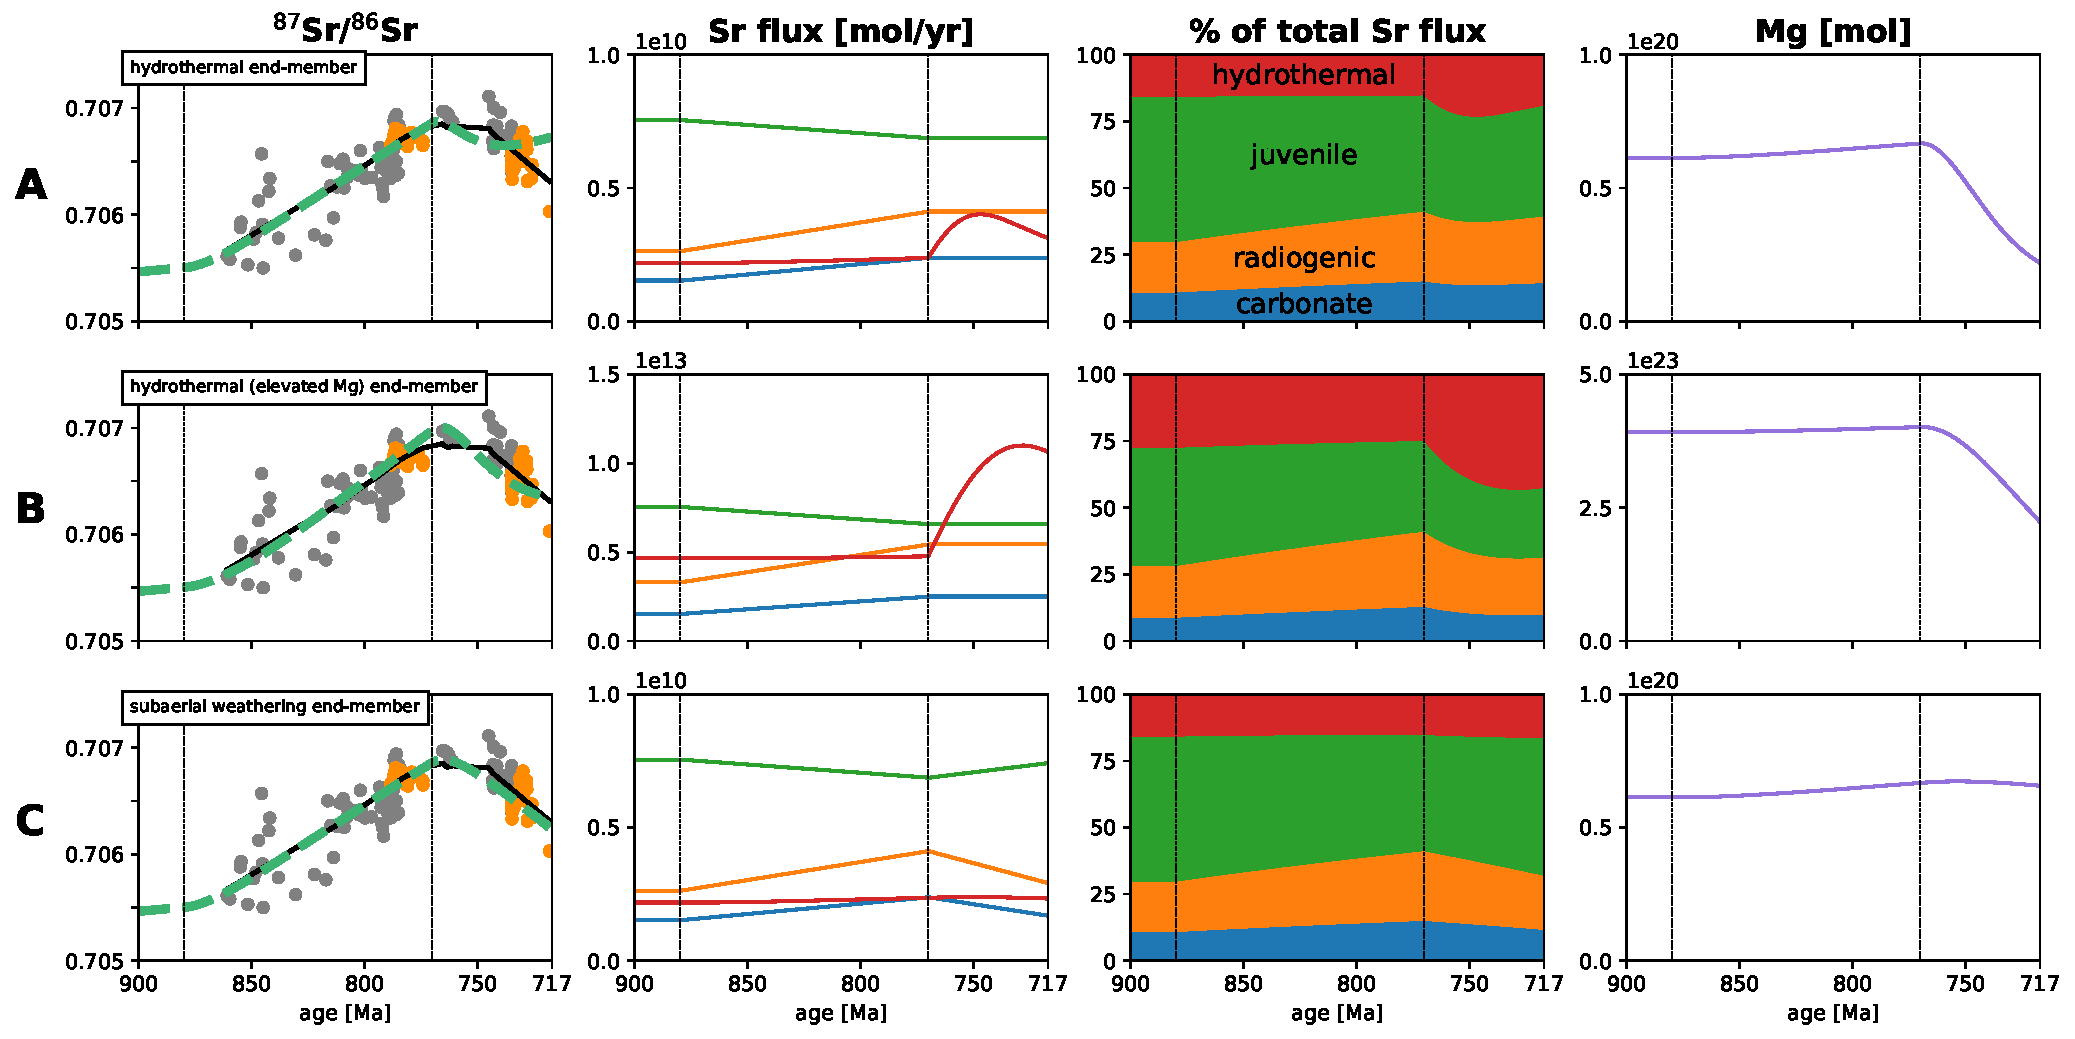
\includegraphics[width=\textwidth]{figures/Tambien/Sr-model-flux-changes.pdf}
	\caption[Tonian global weathering model.]{Global weathering model results. Each row represents a different weathering flux scenario. In the first column, the black curves are the LOWESS fits from Figure \ref{fig:SrSr-LIPs}, and the dashed green curves are the model outputs. Vertical black lines represent times when changes in weathering flux are forced in the model. Each model run has the same weathering flux trajectories from 880 to 770~Ma with varying scenarios between 770~Ma and the onset of Sturtian Glaciation. \textbf{A)} Change in hydrothermal flux only end-member scenario. \textbf{B)} Change in hydrothermal flux only with elevated ocean [Mg] end-member scenario. \textbf{C)} Change in subaerial weathering fluxes only end-member scenario. Note that in the second and fourth columns, scenario B uses different y-axis scales than that used in scenarios A and B.}
	\label{fig:Sr-model-flux-changes}
\end{center}
\end{figure}

The lack of a clear correlation between the LIP record and the ca. 770-717~Ma descent in \SrSr suggests that there are other factors that are driving at least some of the major trends observed in the Tonian \SrSr record. In order to explore these factors, we constructed a simple global weathering model that tracks calcium, magnesium, and strontium fluxes into and out of the ocean. This model is modified from \citet{Maloof2010a} and the Python code that implements it is available in the \SI. The core of the model is based around three equations:

\begin{equation}
  \frac{dCa}{dt} = W_{Ca-carb} + W_{Ca-rad} + W_{Ca-juv} + H_{Ca-basalt} - P_{Ca-carb}
\end{equation}

\begin{equation}
  \frac{dMg}{dt} = W_{Mg-carb} + W_{Mg-rad} + W_{Mg-juv} - H_{Mg-clays} - P_{Mg-carb}
\end{equation}

\begin{equation}
  \frac{dSr}{dt} = W_{^{n}Sr-carb} + W_{^{n}Sr-rad} + W_{^{n}Sr-juv} + H_{^{n}Sr-basalt} - P_{^{n}Sr-carb}
\end{equation}

$W_{X-carb}$, $W_{X-rad}$, and $W_{X-juv}$ are the inputs of Ca, Mg, and Sr coming from subaerial weathering of carbonate ($carb$), radiogenic ($rad$) lithologies, and juvenile ($juv$) lithologies respectively. Each of these terms can be broken down into:

\begin{equation}
	W_{X-lithology} = W_{lithology} \times [X]_{lithology}
\end{equation}

$W_{lithology}$ is the total (all elements) weathering flux coming from the given lithology, and $[X]_{lithology}$ is the average concentration of Ca, Mg, and Sr in the given lithology. $H_{Mg-clays}$ is the loss of Mg in seawater due to the precipitation of clay minerals, $H_{X-basalt}$ is the input of Ca and Sr associated with the weathering of ocean crust during hydrothermal circulation on or near mid-ocean ridges, and $P_{X-carb}$ is the Mg, Ca, and Sr sink associated with the formation of carbonate minerals. $n$ refers to each isotope of Sr ($^{88}$Sr, $^{87}$Sr, $^{86}$Sr). The values of variables used in our model are listed in the \SI. We note that the simple global weathering model used here does not account for changes in seawater chemistry due to dolomitization, which may have acted as a quantitatively significant input/output flux for Mg, Ca, and Sr \citep{Fantle2014a}.

We first spin up the model to steady state over 500~Myr, choosing total Mg, total Ca, $k$, $W_{carb}$, $W_{rad}$, and $W_{juv}$ such that, at the model start age of 880~Ma, Mg/Ca = 10 (based on fluid inclusion data from \citealp{Spear2014a}) and \SrSr = 0.7055 (to match the \SrSr of the time; Fig. \ref{fig:composite-chemostratigraphy}). As a percentage of the total Sr input into the ocean, this model yields hydrothermal = $\sim$15\%, carbonate = $\sim$10\%, radiogenic lithologies = $\sim$20\%, and juvenile lithologies = $\sim$55\% (Fig. \ref{fig:Sr-model-flux-changes}A and B). These initial steady-state Sr fluxes are not a unique solution, and are different than Sr fluxes estimated for the present (hydrothermal = $\sim$10\%, carbonate = $\sim$35\%, radiogenic lithologies = $\sim$25\%, and juvenile lithologies = $\sim$30\%, from \citealp{Allegre2010a}). However, given that modern seawater has a much higher \SrSr ($\sim$0.7091; \citealp{Allegre2010a}) than is estimated for 880~Ma, and Sr fluxes are unconstrained for the Tonian, it is expected, reasonable, and plausible that our initial steady-state Sr fluxes have a higher contribution from juvenile sources (both subaerial weathering of juvenile lithologies and hydrothermal exchange) than is estimated for the present. Furthermore, given that modern seawater has a much lower Mg/Ca (5.2; \citealp{Lowenstein2001a}) than is estimated for the Tonian, it is also expected and reasonable that our initial steady-state Sr fluxes have a lower contribution from carbonate sources than is estimated for the present. After initial spin up to steady state, total silicate (radiogenic and juvenile lithologies) Mg + Ca weathering is held constant throughout the model runs to avoid untenable variations in \textit{p}CO$_{2}$ over million-year time scales \citep{Berner1997a}. We also make the simplifying assumption that carbonate lithologies are distributed homogenously over the globe wherever radiogenic lithologies exist, and thus also hold the ratio of $W_{rad}$ to $W_{carb}$ constant throughout the model runs. We do not expect changes in the carbonate weathering flux to be strongly coupled to changes in the subaerial weathering flux from juvenile lithologies, since carbonate lithologies are not commonly associated with juvenile volcanic rocks erupted as part of a large igneous province. However, these two fluxes may be coupled in the case where basins associated with island arcs have a significant sedimentary carbonate component, and these basins are uplifted and weathered in association with arc amalgamation or arc-continent collision. Our model does not account for this potential coupling, which is a limitation.

From these initial conditions, we sought to explore scenarios that would result in the observed pre-Sturtian Glaciation \SrSr curve. We find that forcing a linear increase in the proportion of the subaerial weathering flux from both the radiogenic lithologies and carbonates ($W_{rad}$ and $W_{carb}$) from $\sim$20\% and $\sim$10\% respectively at 880~Ma to $\sim$25\% and $\sim$15\% respectively at 770~Ma, while decreasing the proportion of the subaerial weathering flux from juvenile lithologies ($W_{juv}$) from $\sim$55\% to $\sim$45\%, produces the increase in \SrSr from ca. 880~Ma (Fig. \ref{fig:Sr-model-flux-changes}A and C). This solution represents a feasible tectonic scenario for this time interval - Rodinia had begun to rift apart at low latitudes during this time \citep{Li2008a}, which would have brought ocean basins in proximity to previously landlocked continental interiors, resulting in as much as an order of magnitude increase in runoff in these areas \citep{Godderis2017a}. The increased runoff in previously arid continental interiors, combined with the generally high runoff and temperature at low latitudes, could have increased the relative weathering flux from radiogenic continental interiors and driven up marine \SrSr between ca. 880-770~Ma, as proposed by \citet{Halverson2007b}. In addition, as discussed above, the `decay' and `weathering' models both predict a small weatherable area of LIPs in the tropics ca. 880-770~Ma relative to the preceding $\sim$230~Myr (Fig. \ref{fig:SrSr-LIPs}D). This tectonic scenario also could have contributed to driving \SrSr to higher values by decreasing the weathering flux from juvenile sources. Since increases or decreases in $W_{rad}$ must be matched by decreases or increases in $W_{juv}$ in order to keep total silicate Mg + Ca weathering constant, the combination of Rodinia rifting apart at low latitudes and a decreasing weatherable area of LIPs within the tropics could have driven \SrSr to higher values. However, significant uncertainty associated with these Tonian paleogeographic reconstructions remain, and this modeled solution is non-unique. Nevertheless, there needs to be an increase in the Sr flux from radiogenic sources relative to juvenile ones to produce the observed increase in \SrSr ca. 880-770~Ma. We note that the rifting of a supercontinent may be associated with an increase in the length of mid-ocean ridges, and therefore an increase in the low \SrSr flux coming from hydrothermal systems (as has been proposed for the opening of the Iapetus Ocean in the Early Cambrian; \citealp{Maloof2010a}). However, since the majority of oceanic crust preserved today is younger than the beginning of the break up of the most recent supercontinent Pangea \citep{Muller2008a}, the effect of supercontinent break up on total mid-ocean ridge length is poorly constrained. Nevertheless, even if the low \SrSr flux coming from hydrothermal systems increased during Rodinia break up, it must have been overwhelmed by the increase in the Sr flux from radiogenic sources in order to drive \SrSr to higher values during this time.

To explain the fall in \SrSr leading into the Sturtian Glaciation, we consider two end-member scenarios. In the first scenario, the absolute flux of H$_{2}$O in hydrothermal systems ($k$) increases, which could represent an increasing length of mid-ocean ridges. In the second scenario, the relative flux coming from the subaerial weathering of juvenile vs. radiogenic lithologies increases, which could represent either an increase in the weatherable area of subaerially exposed LIPs and arcs, a movement/emplacement of LIPs and arcs into higher runoff areas, a movement of radiogenic continental crust into lower runoff areas, or a combination of these forcings.

To replicate the first end-member scenario, we try forcing a 4-fold linear increase in the absolute flux of H$_{2}$O in hydrothermal systems from 770 to 717~Ma (Fig. \ref{fig:Sr-model-flux-changes}A). While this forcing produces a \SrSr curve that matches the initial observed downturn starting at 770~Ma, it later deviates from the observed \SrSr curve and begins rising at ca. 740~Ma. This change in the modeled \SrSr trajectory is a result of depleting seawater of Mg due to the increasing flux of H$_{2}$O in hydrothermal systems. This Mg-depletion reduces hydrothermal Mg-Ca exchange, which in turn reduces the Sr flux coming from hydrothermal alteration \citep{Berndt1988a}. However, since the absolute concentration of ions in seawater is poorly constrained during the Neoproterozoic, we tried to circumvent the problem of depleting [Mg] by changing the initial steady-state conditions such that [Mg] was $\sim$3 orders of magnitude higher than that used in the first model (Fig. \ref{fig:Sr-model-flux-changes}B). Even with this unrealistically large increase in [Mg] (which requires increasing the initial steady-state subaerial weathering flux from juvenile, radiogenic, and carbonate lithologies by 3 orders of magnitude relative to the initial steady-state conditions used in the first model in order to maintain initial Mg/Ca = 10), a $\sim$4-fold increase in the absolute flux of H$_{2}$O in hydrothermal systems from 770 to 717~Ma is still required to match the observed \SrSr curve. As discussed above, it is unclear how supercontinent break up effects the total length of mid-ocean ridges, but a 4-fold increase in this length should be unrealistically large, especially when we consider that mid-ocean ridges outside of Rodinia existed independent of the break-up of the supercontinent. The Arabian-Nubian Shield itself comprises at least 10 distinct tectonostratigraphic island arc terranes that accreted onto the periphery of Rodinia \citep{Johnson2014a} resulting from active seafloor spreading. Furthermore, if the hypothesis that rifting played an important role in increasing the Sr flux coming from radiogenic lithologies ca. 880-770~Ma is correct, the associated possible increase in the length of mid-ocean ridges would have preceded the decline in \SrSr going into the glaciation.

To replicate the second end-member scenario, we found that forcing a linear increase in the subaerial weathering flux from juvenile lithologies from $\sim$45\% at 770~Ma to $\sim$55\% at 717~Ma (while keeping total silicate Mg + Ca weathering constant) produces the decrease in \SrSr from ca. 770~Ma leading into the Sturtian Glaciation (Fig. \ref{fig:Sr-model-flux-changes}C).

Together, these three global weathering model scenarios (Fig. \ref{fig:Sr-model-flux-changes}) suggest that the primary driver of decreasing \SrSr leading into the Sturtian Glaciation was the second end-member scenario -- an increasing relative flux coming from the subaerial weathering of juvenile lithologies, rather than an increase in the absolute flux of H$_{2}$O in hydrothermal systems. However, as discussed above, all three post-emplacement models in Figure \ref{fig:SrSr-LIPs}D place a roughly stable area of weatherable LIPs in the tropics ca. 880-720~Ma. Therefore, an increase in the weathering flux from LIPs is likely not the primary driver for increasing the relative flux coming from the weathering of juvenile lithologies starting ca. 770~Ma. Furthermore, current paleogeographic reconstructions overall suggest that Rodinia continued to rift apart at low latitudes ca. 770-717~Ma (e.g. \citealp{Li2008a}) in a manner similar to that described above for ca. 880-770~Ma. Such plate motions would not lead to any significant increase of `continentality' or movement of continental crust into higher latitudes ca. 770-717~Ma, and therefore an associated decrease in the weathering flux from radiogenic continental crust as a result of these processes is not expected.

\subsubsection{Arc Accretion}

A potential driver of the ca. 770~Ma inflection in the \SrSr record is the first episode of Arabian-Nubian arc accretion along the Bi'r Umq-Nakasib Suture -- estimated to have occurred ca. 780-760~Ma based on the ages of terrane protoliths and of syn- and post-tectonic intrusions (\citealp{Pallister1988a, Johnson2003a, Johnson2003b, Johnson2014a}; Fig. \ref{fig:SrSr-LIPs}E). This accretion event represents a difference between ca. 880-770~Ma and ca. 770-720~Ma, and was followed by accretion along the Allaqi-Heiani-Yanbu Suture -- estimated to have occurred ca. 730-710~Ma based on the ages of terrane protoliths and post-tectonic intrusions \citep{Ali2010a, Johnson2014a, Kozdroj2017a}. The paleolatitude of this accretion and associated exhumation is poorly constrained. However, the record of Arabian-Nubian arc accretion during the late Neoproterozoic assembly of Gondwana suggests that the Arabian-Nubian arc terranes were situated between India and the Congo + Saharan cratons \citep{Li2008a, Hoffman2009a, Merdith2017a}. This position leads to a low to mid-latitude position at the time of the ca. 780-760~Ma accretion event within paleogeographic models (e.g. \citealp{Li2008a,  Merdith2017a}; Fig. \ref{fig:SrSr-LIPs}E). A tropical position of proto-Arabian-Nubian Shield arc terranes is consistent with the interpreted depositional environment of the Tambien Group, given the abundance of carbonate lithofacies such as oolite which are indicative of warm waters that are supersaturated with respect to calcium carbonate (Fig. \ref{fig:fence-diagram}). Exhumation associated with arc terrane collision would have led to the development of steep topography and high rates of physical erosion and chemical weathering \citep{Gabet2009a}. The high concentrations of Ca and Mg in the uplifted rocks make it so they would have had high carbon sequestration potential. The development of topography also generates a physical barrier that forces air masses to rise and cool, which should result in an increase in the local precipitation, supplementing the already high precipitation in the tropics. Together, these factors could have substantially increased the weathering flux coming from these juvenile island arcs. Given that the LIP analysis (Fig. \ref{fig:SrSr-LIPs}D) suggests that an increase in the weathering flux from LIPs ca. 880-720~Ma is unlikely, this episode of Arabian-Nubian arc accretion stands as a strong candidate for the primary driver for falling \SrSr starting ca. 770~Ma.

Other major ca. 1300-700~Ma arc accretion events that can be identified in the geological record (Fig. \ref{fig:SrSr-LIPs}E) include: the ca. 1204-1174~Ma accretion of the Pie de Palo Complex \citep{Vujovich1998a, Vujovich2004a} and the ca. 1200-1160~Ma accretion of the Pyrites Ophiolite Complex \citep{McLelland2013a} onto Laurentia during the Shawinigan Orogeny, the ca. 870-813~Ma accretion of the Miaowan Ophiolite onto the northern margin of the Yangtze block of South China \citep{Peng2012a}, the ca. 825-815~Ma Jiangnan Orogen associated with the closure of the ocean basin between the terranes of the Yangtze and Cathaysia blocks that make up South China \citep{Zhao2015a}, and the ca. 820-800~Ma closure of the ocean basin between the Greater India landmass and the Marwar craton \citep{Volpe1990a, Chatterjee2017a}. However, paleomagnetic poles place Laurentia \citep{Palmer1977a, Buchan2000a}, South China \citep{Li2004a, Niu2016a}, and India \citep{Meert2013a} outside of the tropics at or near the time of these accretion events, indicating that exhumation of associated mafic lithologies would have occurred at mid- to high latitudes with a correspondingly muted influence on global weathering and \SrSr values compared to the Arabian-Nubian events (Fig. \ref{fig:SrSr-LIPs}). We note, however, that this compilation of ca. 1300-700~Ma arc accretion events (Fig. \ref{fig:SrSr-LIPs}E) is limited to the current literature on ophiolite-bearing sutures. Additional arc accretion events associated with the late Mesoproterozoic-early Neoproterozoic assembly of Rodinia \citep{Cawood2016a}, may not be preserved due to exhumation and erosion. Therefore, while it is possible that Arabian-Nubian arc accretion is unique in terms of a low-latitude position in this time interval, such a conclusion would be premature.

By appreciating that arc accretion, especially in the tropics, has the potential to contribute sufficient solutes to the global weathering flux to alter global marine \SrSr for tens of millions of years, we can examine the factors that contributed to the ca. 717~Ma initiation of the Sturtian Glaciation from a fresh perspective. Age constraints on the emplacement of the Franklin LIP into the tropics (Fig. \ref{fig:SrSr-LIPs}C and D) cluster at ca. 720~Ma, but range from ca. 723~Ma to ca. 712~Ma \citep{Heaman1992a, Pehrsson1999a, Denyszyn2009a}. Without tighter age constraints on the timing of this emplacement, interpreting its precise relationship to the ca. 717~Ma initiation of the Sturtian Glaciation is difficult. If the emplacement precisely coincided with the initiation of the Sturtian Glaciation, then its primary contribution to initiating Snowball Earth could have been through cooling associated with the injection of sulfur aerosols into the stratosphere \citep{Macdonald2017a}. On the other hand, if the emplacement preceded the initiation by $\sim$1~Myr or more, then its contribution to it would have been to enhance planetary weatherability \citep{Godderis2003a, Rooney2014a, Cox2016a}, since the residence time of sulfur aerosols in the stratosphere is less than a few years \citep{McCormick1995a}. Regardless of the precise nature of this relationship, our LIP area analysis (Fig. \ref{fig:SrSr-LIPs}C and D) indicates that the Franklin LIP does not correspond to a uniquely large LIP area in the tropics. While it is one of the two highest peaks of tropical LIP area in the 1300-700~Ma interval, a larger area of weatherable LIP is reconstructed to have existed both globally and within the tropics at ca. 1100~Ma due to the Umkondo LIP, comparable in size to the Franklin LIP, being emplaced in the tropics ca. 1110~Ma, as well as the migration of the SW Laurentia LIP into the tropics at this time. Furthermore, larger areas of weatherable LIP than both the Umkondo and Franklin LIPs have been reconstructed to exist within the tropics several more times in the Phanerozoic \citep{Park2019a}. Given that there were no Snowball Earth glaciations ca. 1100~Ma or in the Phanerozoic despite there being larger areas of weatherable LIPs emplaced within the tropics than ca. 717~Ma, it is difficult to explain the initiation of the Sturtian Glaciation with the Franklin LIP alone.

However, what may differentiate the interval preceding the Sturtian Glaciation and ca. 1100~Ma are the pair of Arabian-Nubian arc accretion events that potentially occured in the tropics (Fig. \ref{fig:SrSr-LIPs}E). Within this context, the Franklin LIP was not solely responsible for cooling Earth to the threshold required to initiate global glaciation. Rather, as suggested by the \SrSr record, we propose that Arabian-Nubian arc accretion in the tropics enhanced planetary weatherability and lowered atmospheric CO$_{2}$ concentration over the $\sim$50~Myr prior to the initiation of the Sturtian Glaciation. The Franklin LIP then was emplaced in the tropics into an already cool planet, and its additional cooling effect, either through CO$_{2}$ consumption via silicate weathering and/or cooling associated with the injection of sulfur aerosols, may have tipped the climate over the threshold required for the ice-albedo positive feedback to overwhelm negative feedbacks on cooling and initiate global glaciation. Therefore, Arabian-Nubian arc accretion may have worked together with LIP emplacement to allow global glaciation to occur, and that without this arc exhumation, the Sturtian Glaciation may not have occurred. Subsequent arc accretion events within the Arabian Shield in the Cryogenian \citep{Johnson2014a} may have played a role in elevating planetary weatherability and contributing to the onset of the Marinoan Glaciation as well. Other studies also have argued that tropical arc accretion events contributed to global cooling in the Eocene, Cretaceous \citep{Jagoutz2016a}, and Ordovician \citep{Swanson-Hysell2017a} - a correlation that appears robust throughout the Phanerozoic \citep{Macdonald2019a}. Crucially, this hypothesis hinges on the paleogeographic position of these Arabian-Nubian arc accretion events to sufficiently increase planetary weatherability. Direct paleomagnetic data that provides such constraints should be a priority for future research. Furthermore, the LIP and arc accretion analysis presented here is limited to ca. 1300-700~Ma, and extending this analysis to the rest of Earth history is necessary to further evaluate the uniqueness of the combination of tropical LIPs, tropical arc accretion events, and global cooling.

\section{Conclusions}

The Tambien Group was deposited for over 100 million years of Tonian Earth history leading into the Sturtian Glaciation. The presence of carbonates and tuffs throughout the strata enable the generation of temporally well-constrained chemostratigraphic data leading into the first of the Cryogenian glaciations. U-Pb ID-TIMS ages indicate that Tambien Group carbonates were deposited from ca. 820~Ma until 0 to 2~Myr before the onset of the Sturtian Glaciation, making the group host to the most complete carbonate stratigraphy leading into this glaciation that has been constrained with geochronology. We have used new \dC and \SrSr data and U-Pb ID-TIMS ages from the Tambien Group to construct the most temporally well-constrained Tonian composite chemostratigraphic dataset to date, and used it to show: 1) that the 735~Ma anomaly is synchronous in at least two separate basins, precedes the Sturtian Glaciation by $\sim$18~Myr, and is followed by a prolonged interval of positive \dC values; 2) low-latitude glaciation was likely rapid leading into the Sturtian Glaciation, as predicted by energy balance models; and 3) enhanced subaerial weathering of juvenile lithologies, and an associated increase in weatherability that would have lowered CO$_{2}$, began $\sim$50~Myr prior to the initiation of the Sturtian Glaciation. The accretion of Arabian-Nubian Shield volcanic arcs in the tropics during this time likely played an important role in increasing global weatherability, contributing to the initiation of the first Neoproterozoic Snowball Earth.

\section{Acknowledgements}

Research funding came from the U.S. National Science Foundation grants EAR-1325230 (Swanson-Hysell) and EAR-1323158 (Maloof). Tremblay was supported by an U.S. National Science Foundation Graduate Research Fellowship. Sr isotope data were collected in the Center for Isotope Geochemistry at UC Berkeley directed by Don DePaolo, which is supported by the Director, Office of Science, Office of Basic Energy Sciences, of the U.S. Department of Energy under contract number DE-AC02-05CH11231. Acknowledgement and thanks go to Shaun Brown and Thomas Owens for assisting with the development of Sr isotope data, to Wenbo Yang for assisting with the development of element concentration data, Samantha Gwizd, Sergey Oleynik, and Disha Okhai for assisting with the development of C and O isotope data, and Sara Beroff for assisting with the development of the molar tooth structure petrographic data with support from the Cal NERDS program. Gawen Jenkin helped introduce Swanson-Hysell and Maloof to the Tambien Group. Daniel Condon was instrumental in generating previous U-Pb dates on the Tambien Group that was built-upon in the current work.